\documentclass[a4paper]{amsbook}
\usepackage[utf8]{inputenc}
\usepackage[T1]{fontenc}
\usepackage[pdftex]{graphicx}

\title{Great Speeches}
\author{Organization: Brett \& Kate McKay \\
         Formatting: Andr\'{e} Wagner}
\date{}

\begin{document}

\maketitle
\tableofcontents
\chapter{Pericles - Funeral Oration}

\textbf{\Large{Athens -- 431 B.C.}}

\vspace{10 mm}

\begin{figure}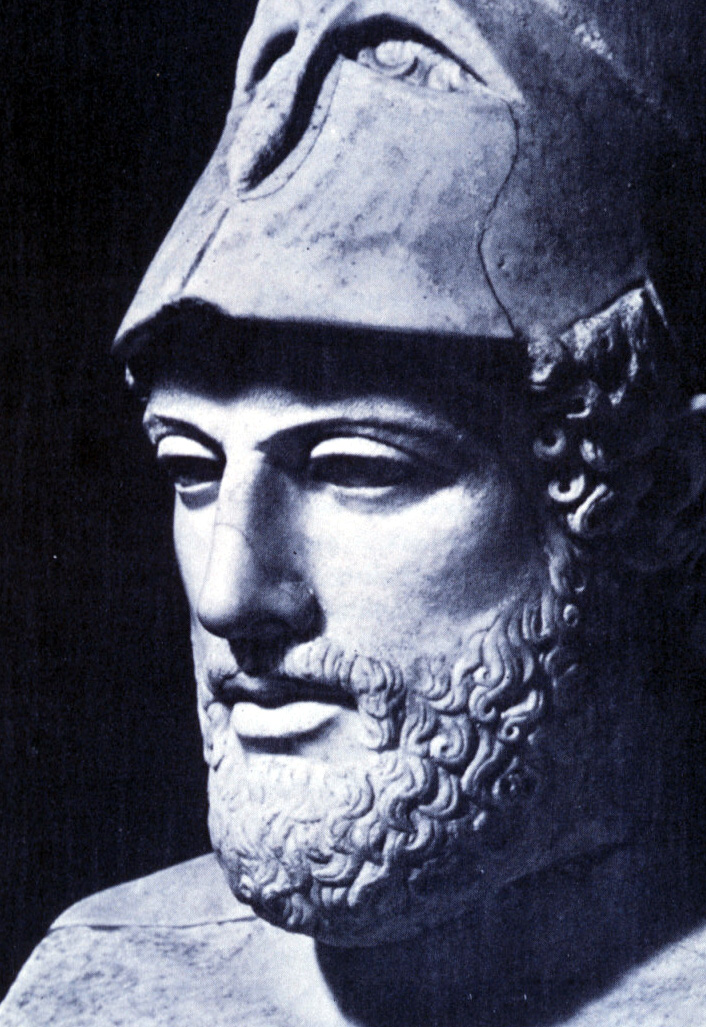
\includegraphics[width=0.6\textwidth]{pericles.jpg}\end{figure}
{\em Pericles, master statesman, orator, and general, was truly, as Thuciydies dubbed him, “the first citizen of Athens.” Pericles was a product of the Sophists and had been personally tutored by the great philosopher Anaxagoras. His study with the Sophists made Pericles a highly persuasive orator. Through his speeches, he galvanized Athenians to undertake an enormous public works project that created hundreds of temples, including the Pantheon.

Pericles' gift of oration was put to the test during the epic battles of the Peloponnesian War, a civil war between Athens and Sparta. His speeches inspired Athenians to fight to become the number one power in Greece. In February of 431 B.C., Athens had their annual public funeral to honor all those who died in war. Pericles was asked to give the traditional funeral oration. Rather than focus his speech on enumerating the conquests of Athens' fallen heroes, Pericles instead used his funeral oration to laud the glory of Athens itself and inspire the living to make sure the soldiers had not died in vain.

Over 2,000 years later, Pericles' funeral oration inspired Abraham Lincoln's “Gettysburg Address.” Like Pericles, Lincoln was a leader during a time of civil war. Like Pericles, Lincoln focused on exhorting the living to live their lives in a way that would make the sacrifice of fallen warriors worthwhile.}

\vspace{10 mm}

Most of my predecessors in this place have commended him who made this speech part of the law, telling us that it is well that it should be delivered at the burial of those who fall in battle. For myself, I should have thought that the worth which had displayed itself in deeds would be sufficiently rewarded by honors also shown by deeds; such as you now see in this funeral prepared at the people's cost. And I could have wished that the reputations of many brave men were not to be imperiled in the mouth of a single individual, to stand or fall according as he spoke well or ill. For it is hard to speak properly upon a subject where it is even difficult to convince your hearers that you are speaking the truth. On the one hand, the friend who is familiar with every fact of the story may think that some point has not been set forth with that fullness which he wishes and knows it to deserve; on the other, he who is a stranger to the matter may be led by envy to suspect exaggeration if he hears anything above his own nature. For men can endure to hear others praised only so long as they can severally persuade themselves of their own ability to equal the actions recounted: when this point is passed, envy comes in and with it incredulity. However, since our ancestors have stamped this custom with their approval, it becomes my duty to obey the law and to try to satisfy your several wishes and opinions as best I may.

I shall begin with our ancestors: it is both just and proper that they should have the honor of the first mention on an occasion like the present. They dwelt in the country without break in the succession from generation to generation, and handed it down free to the present time by their valor. And if our more remote ancestors deserve praise, much more do our own fathers, who added to their inheritance the empire which we now possess, and spared no pains to be able to leave their acquisitions to us of the present generation. Lastly, there are few parts of our dominions that have not been augmented by those of us here, who are still more or less in the vigor of life; while the mother country has been furnished by us with everything that can enable her to depend on her own resources whether for war or for peace. That part of our history which tells of the military achievements which gave us our several possessions, or of the ready valour with which either we or our fathers stemmed the tide of Hellenic or foreign aggression, is a theme too familiar to my hearers for me to dilate on, and I shall therefore pass it by. But what was the road by which we reached our position, what the form of government under which our greatness grew, what the national habits out of which it sprang; these are questions which I may try to solve before I proceed to my panegyric upon these men; since I think this to be a subject upon which on the present occasion a speaker may properly dwell, and to which the whole assemblage, whether citizens or foreigners, may listen with advantage.

Our constitution does not copy the laws of neighboring states; we are rather a pattern to others than imitators ourselves. Its administration favors the many instead of the few; this is why it is called a democracy. If we look to the laws, they afford equal justice to all in their private differences; if no social standing, advancement in public life falls to reputation for capacity, class considerations not being allowed to interfere with merit; nor again does poverty bar the way, if a man is able to serve the state, he is not hindered by the obscurity of his condition. The freedom which we enjoy in our government extends also to our ordinary life. There, far from exercising a jealous surveillance over each other, we do not feel called upon to be angry with our neighbor for doing what he likes, or even to indulge in those injurious looks which cannot fail to be offensive, although they inflict no positive penalty. But all this ease in our private relations does not make us lawless as citizens. Against this fear is our chief safeguard, teaching us to obey the magistrates and the laws, particularly such as regard the protection of the injured, whether they are actually on the statute book, or belong to that code which, although unwritten, yet cannot be broken without acknowledged disgrace.

Further, we provide plenty of means for the mind to refresh itself from business. We celebrate games and sacrifices all the year round, and the elegance of our private establishments forms a daily source of pleasure and helps to banish the spleen; while the magnitude of our city draws the produce of the world into our harbour, so that to the Athenian the fruits of other countries are as familiar a luxury as those of his own.

If we turn to our military policy, there also we differ from our antagonists. We throw open our city to the world, and never by alien acts exclude foreigners from any opportunity of learning or observing, although the eyes of an enemy may occasionally profit by our liberality; trusting less in system and policy than to the native spirit of our citizens; while in education, where our rivals from their very cradles by a painful discipline seek after manliness, at Athens we live exactly as we please, and yet are just as ready to encounter every legitimate danger. In proof of this it may be noticed that the Lacedaemonians do not invade our country alone, but bring with them all their confederates; while we Athenians advance unsupported into the territory of a neighbor, and fighting upon a foreign soil usually vanquish with ease men who are defending their homes. Our united force was never yet encountered by any enemy, because we have at once to attend to our marine and to dispatch our citizens by land upon a hundred different services; so that, wherever they engage with some such fraction ofour strength, a success against a detachment is magnified into a victory over the nation, and a defeat into a reverse suffered at the hands of our entire people. And yet if with habits not of labor but of ease, and courage not of art but of nature, we are still willing to encounter danger, we have the double advantage of escaping the experience of hardships in anticipation and of facing them in the hour of need as fearlessly as those who are never free from them.

Nor are these the only points in which our city is worthy of admiration. We cultivate refinement without extravagance and knowledge without effeminacy; wealth we employ more for use than for show, and place the real disgrace of poverty not in owning to the fact but in declining the struggle against it. Our public men have, besides politics, their private affairs to attend to, and our ordinary citizens, though occupied with the pursuits of industry, are still fair judges of public matters; for, unlike any other nation, regarding him who takes no part in these duties not as unambitious but as useless, we Athenians are able to judge at all events if we cannot originate, and, instead of looking on discussion as a stumbling-block in the way of action, we think it an indispensable preliminary to any wise action at all.

Again, in our enterprises we present the singular spectacle of daring and deliberation, each carried to its highest point, and both united in the same persons; although usually decision is the fruit of ignorance, those, who best know the difference between hardship and pleasure and yet are never tempted to shrink from danger. In generosity we are equally singular, acquiring our friends by conferring, not by receiving, favours. Yet, of course, the doer of the favo is the firmer friend of the two, in order by continued kindness to keep the recipient in his debt; while the debtor feels less keenly from the very consciousness that the return he makes will be a payment, not a free gift. And it is only the Athenians, who, fearless of consequences, confer their benefits not from calculations of expediency, but in the confidence of liberality.

In short, I say that as a city we are the school of Hellas, while I doubt if the world can produce a man who, where he has only himself to depend upon, is equal to so many emergencies, and graced by so happy a versatility, as the Athenian. And that this is no mere boast thrown out for the occasion, but plain matter of fact, the power of the state acquired by these habits proves. For Athens alone of her contemporaries is found when tested to be greater than her reputation, and alone gives no occasion to her assailants to blush at the antagonist by whom they have been worsted, or to her subjects to question her title by merit to rule. Rather, the admiration of the present and succeeding ages will be ours, since we have not left our power without witness, but have shown it by mighty proofs; and far from needing a Homer for our panegyrist, or other of his craft whose verses might charm for the moment only for the impression which they gave to melt at the touch of fact, we have forced every sea and land to be the highway of our daring, and everywhere, whether for evil or for good, have left imperishable monuments behind us. Such is the Athens for which these men, in the assertion of their resolve not to lose her, nobly fought and died; and well may every one of their survivors be ready to suffer in her cause.

Indeed if I have dwelt at some length upon the character of our country, it has been to show that our stake in the struggle is not the same as theirs who have no such blessings to lose, and also that the panegyric of the men over whom I am now speaking might be by definite proofs established. That panegyric is now in a great measure complete; for the Athens that I have celebrated is only what the heroism of these and their like have made her, men whose fame, unlike that of most Hellenes, will be found to be only commensurate with their deserts. And if a test of worth be wanted, it is to be found in their closing scene, and this not only in cases in which it set the final seal upon their merit, but also in those in which it gave the first intimation of their having any. For there is justice in the claim that steadfastness in his country's battles should be as a cloak to cover a man's other imperfections; since the good action has blotted out the bad, and his merit as a citizen more than outweighed his demerits as an individual. But none of these allowed either wealth with its prospect of future enjoyment to unnerve his spirit, or poverty with its hope of a day of freedom and riches to tempt him to shrink from danger.

No, holding that vengeance upon their enemies was more to be desired than any personal blessings, and reckoning this to be the most glorious of hazards, they joyfully determined to accept the risk, to make sure of their vengeance, and to let their wishes wait; and while committing to hope the uncertainty of final success, in the business before them they thought fit to act boldly and trust in themselves. Thus choosing to die resisting, rather than to live submitting, they fled only from dishonour, but met danger face to face, and after one brief moment, while at the summit of their fortune, escaped, not from their fear, but from their glory.

Athena Mourning”So died these men as became Athenians. You, their survivors, must determine to have as unfaltering a resolution in the field, though you may pray that it may have a happier issue. And not contented with ideas derived only from words of the advantages which are bound up with the defence of your country, though these would furnish a valuable text to a speaker even before an audience so alive to them as the present, you must yourselves realize the power of Athens, and feed your eyes upon her from day to day, till love of her fills your hearts; and then, when all her greatness shall break upon you, you must reflect that it was by courage, sense of duty, and a keen feeling of honor in action that men were enabled to win all this, and that no personal failure in an enterprise could make them consent to deprive their country of their valor, but they laid it at her feet as the most glorious contribution that they could offer. [Image: Athena mourning a dead Greek hero; fifth-century marble relief in the Acropolis Museum.]

For this offering of their lives made in common by them all they each of them individually received that renown which never grows old, and for a sepulcher, not so much that in which their bones have been deposited, but that noblest of shrines wherein their glory is laid up to be eternally remembered upon every occasion on which deed or story shall call for its commemoration. For heroes have the whole earth for their tomb; and in lands far from their own, where the column with its epitaph declares it, there is enshrined in every breast a record unwritten with no tablet to preserve it, except that of the heart. These take as your model and, judging happiness to be the fruit of freedom and freedom of valour, never decline the dangers of war. For it is not the miserable that would most justly be unsparing of their lives; these have nothing to hope for: it is rather they to whom continued life may bring reverses as yet unknown, and to whom a fall, if it came, would be most tremendous in its consequences. And surely, to a man of spirit, the degradation of cowardice must be immeasurably more grievous than the unfelt death which strikes him in the midst of his strength and patriotism!

Comfort, therefore, not condolence, is what I have to offer to the parents of the dead who may be here. Numberless are the chances to which, as they know, the life of man is subject; but fortunate indeed are they who draw for their lot a death so glorious as that which has caused your mourning, and to whom life has been so exactly measured as to terminate in the happiness in which it has been passed. Still I know that this is a hard saying, especially when those are in question of whom you will constantly be reminded by seeing in the homes of others blessings of which once you also boasted: for grief is felt not so much for the want of what we have never known, as for the loss of that to which we have been long accustomed. Yet you who are still of an age to beget children must bear up in the hope of having others in their stead; not only will they help you to forget those whom you have lost, but will be to the state at once a reinforcement and a security; for never can a fair or just policy be expected of the citizen who does not, like his fellows, bring to the decision the interests and apprehensions of a father. While those of you who have passed your prime must congratulate yourselves with the thought that the best part of your life was fortunate, and that the brief span that remains will be cheered by the fame of the departed. For it is only the love of honour that never grows old; and honor it is, not gain, as some would have it, that rejoices the heart of age and helplessness.

Turning to the sons or brothers of the dead, I see an arduous struggle before you. When a man is gone, all are wont to praise him, and should your merit be ever so transcendent, you will still find it difficult not merely to overtake, but even to approach their renown. The living have envy to contend with, while those who are no longer in our path are honored with a goodwill into which rivalry does not enter.

On the other hand, if I must say anything on the subject of female excellence to those of you who will now be in widowhood, it will be all comprised in this brief exhortation. Great will be your glory in not falling short of your natural character; and greatest will be hers who is least talked of among the men, whether for good or for bad.

My task is now finished. I have performed it to the best of my ability, and in word, at least, the requirements of the law are now satisfied. If deeds be in question, those who are here interred have received part of their honors already, and for the rest, their children will be brought up till manhood at the public expense: the state thus offers a valuable prize, as the garland of victory in this race of valor, for the reward both of those who have fallen and their survivors. And where the rewards for merit are greatest, there are found the best citizens.

And now that you have brought to a close your lamentations for your relatives, you may depart.


\chapter{Demosthenes - The Third Philippic}

\textbf{\Large{Athens, Greece -- 342 B.C.}}

\vspace{10 mm}

\begin{figure}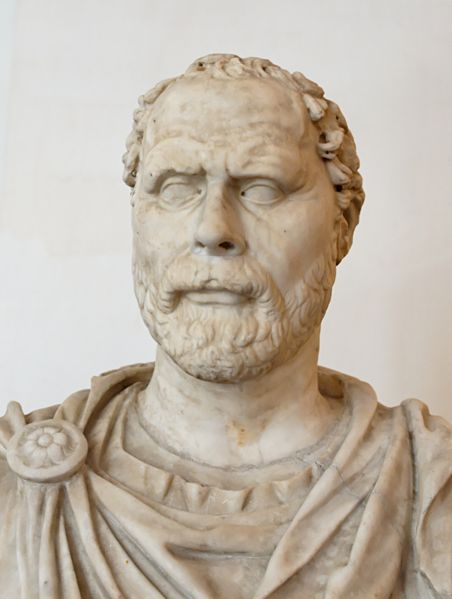
\includegraphics[width=0.6\textwidth]{452px-demosthenes_altemps_inv8581.jpg}\end{figure}
{\em Demosthenes, master statesman and orator, loved his city-state of Athens. He cherished its way of life and abundant freedoms. And he believed in standing strong against anyone who might attempt to infringe on these privileges. This passion, unfortunately, was seldom shared by his fellow Athenians. While Philip the II of Macedon made bolder and bolder incursions into the Greek peninsula, the Athenian people seemed stuck in an apathetic stupor. For years, Demosthenes employed his powerful oratorical skills in attempts to awaken his fellow citizens from sleep to the realization of the imminent danger Philip posed. When Philip advanced on Thrace, the Athenians called an assembly to debate whether or not to finally heed the great orator's advice. Demosthenes was sick of his brethren taking liberty and the Athenian way of life for granted and he boldly called upon them to rise up and take action. After his rousing speech, the assembly all cried out, “To arms! To arms!”}

\vspace{10 mm}

Many speeches are made, men of Athens, at almost every meeting of the Assembly, with reference to the aggressions which Philip has been committing, ever since he concluded the Peace, not only against yourselves but against all other peoples.

And I am sure that all would agree, however little they may act on their belief, that our aim, both in speech and in action, should be to cause him to cease from his insolence and to pay the penalty for it. And yet I see that in fact the treacherous sacrifice of our interests has gone on, until what seems an ill-omened saying may, I fear, be really true - that if all who came forward desired to propose, and you desired to carry, the measures which would make your position as pitiful as it could possibly be, it could not, so I believe, be made worse than it is now.

It may be that there are many reasons for this, and that our affairs did not reach their present condition from any one or two causes. But if you examine the matter aright, you will find that the chief responsibility rests with those whose aim is to win your favor, not to propose what is best. Some of them, men of Athens, so long as they can maintain the conditions which bring them reputation and influence, take no thought for the future and therefore think that you also should take none, while others, by accusing and slandering those who are actively at work, are simply trying to make the city spend its energies in punishing the members of its own body, and so leave Philip free to say and do what he likes.

Such political methods as these, familiar to you as they are, are the real causes of the evil. And I beg you, men of Athens, if I tell you certain truths outspokenly, to let no resentment on your part fall upon me on this account. Consider the matter in this light. In every other sphere of life, you believe that the right of free speech ought to be so universally shared by all who are in the city, that you have extended it both to foreigners and to slaves; and one may see many a servant in Athens speaking his mind with greater liberty than is granted to citizens in some other states: but from the sphere of political counsel you have utterly banished this liberty.

The result is that in your meetings you give yourselves airs and enjoy their flattery, listening to nothing but what is meant to please you, while in the world of facts and events, you are in the last extremity of peril. If then you are still in this mood to-day, I do not know what I can say; but if you are willing to listen while I tell you, without flattery, what your interest requires, I am prepared to speak. For though our position is very bad indeed, and much has been sacrificed, it is still possible, even now, if you will do your duty, to set all right once more.

It is a strange thing, perhaps, that I am about to say, but it is true. The worst feature in the past is that in which lies our best hope for the future. And what is this? It is that you are in your present plight because you do not do any part of your duty, small or great; for of course, if you were doing all that you should do, and were still in this evil case, you could not even hope for any improvement. As it is, Philip has conquered your indolence and your indifference; but he has not conquered Athens. You have not been vanquished, you have never even stirred.

Now if it was admitted by us all that Philip was at war with Athens, and was transgressing the Peace, a speaker would have to do nothing but to advise you as to the safest and easiest method of resistance to him. But since there are some who are in so extraordinary a frame of mind that, though he is capturing cities, though many of your possessions are in his hands, and though he is committing aggressions against all men, they still tolerate certain speakers, who constantly assert at your meetings that it is some of us who are provoking the war, it is necessary to be on our guard and come to a right understanding on the matter.

For there is a danger lest any one who proposes or advises resistance should find himself accused of having brought about the war. Well, I say this first of all, and lay it down as a principle, that if it is open to us to deliberate whether we should remain at peace or should go to war \ldots

Now if it is possible for the city to remain at peace, if the decision rests with us that I may make this my starting-point, then I say that we ought to do so, and I call upon any one who says that it is so to move his motion, and to act and not to defraud us. But if another with weapons in his hands and a large force about him holds out to you the name of peace while his own acts are acts of war what course remains open to us but that of resistance?

Though if you wish to profess peace in the same manner as he, I have no quarrel with you. But if any man's conception of peace is that it is a state in which Philip can master all that intervenes till at last he comes to attack ourselves, such a conception, in the first place, is madness; and, in the second place, this peace that he speaks of is a peace which you are to observe towards Philip, while he does not observe it towards you: and this it is, this power to carry on war against you, without being met by any hostilities on your part, that Philip is purchasing with all the money that he is spending.

Indeed, if we intend to wait till the time comes when he admits that he is at war with us, we are surely the most innocent persons in the world. Why, even if he comes to Attica itself, to the very Peiraeus, he will never make such an admission, if we are to judge by his dealings with others.

For, to take one instance, he told the Olynthians, when he was five miles from the city, that there were only two alternatives, either they must cease to live in Olynthus, or he to live in Macedonia: but during the whole time before that, whenever any one accused him of any such sentiments, he was indignant and sent envoys to answer the charge. Again, he marched into the Phocians' country, as though visiting his allies. It was by Phocian envoys that he was escorted on the march; and most people in Athens contended strongly that his crossing the Pass would bring no good to Thebes.

Worse still, he has lately seized Pherae and still holds it, though he went to Thessaly as a friend and an ally. And, latest of all, he told those unhappy citizens of Oreus that he had sent his soldiers to visit them and to make kind inquiries; he had heard that they were sick, and suffering from faction, and it was right for an ally and a true friend to be present at such a time.

Now if, instead of giving them warning and using open force, he deliberately chose to deceive these men, who could have done him no harm, though they might have taken precautions against suffering any themselves, do you imagine that he will make a formal declaration of war upon you before he commences hostilities, and that, so long as you are content to be deceived? Impossible! For so long as you, though you are the injured party, make no complaint against him, but accuse some of your own body, he would be the most fatuous man on earth if he were to interrupt your strife and contentions with one another, to bid you turn upon himself, and so to cut away the ground from the arguments by which his hirelings put you off, when they tell you that he is not at war with Athens.

In God's name, is there a man in his senses who would judge by words, and not by facts, whether another was at peace or at war with him? Of course there is not. Why, from the very first, when the Peace had only just been made, before those who are now in the Chersonese had been sent out, Philip was taking Serrhium and Doriscus, and expelling the soldiers who were in the castle of Serrhium and the Sacred Mountain, where they had been placed by your general. But what was he doing, in acting thus? For he had sworn to a Peace. And let no one ask, What do these things amount to? What do they matter to Athens?

For whether these acts were trifles which could have no interest for you is another matter; but the principles of religion and justice, whether a man transgress them in small things or great, have always the same force. What? When he is sending mercenaries into the Chersonese, which the king and all the Hellenes have acknowledged to be yours; when he openly avows that he is going to the rescue, and states it in his letter, what is it that he is doing?

He tells you, indeed, that he is not making war upon you. But so far am I from admitting that one who acts in this manner is observing the Peace which he made with you, that I hold that in grasping at Megara, in setting up tyrants in Euboea, in advancing against Thrace at the present moment, in pursuing his machinations in the Peloponnese, and in carrying out his entire policy with the help of his army, he is violating the Peace and is making war against you. Unless you mean to say that even to bring up engines to besiege you is no breach of the Peace, until they are actually planted against your walls. But you will not say this; for the man who is taking the steps and contriving the means which will lead to my capture is at war with me, even though he has not yet thrown a missile or shot an arrow.

Now what are the things which would imperil your safety, if anything should happen? The alienation of the Hellespont, the placing of Megara and Euboea in the power of the enemy, and the attraction of Peloponnesian sympathy to his cause. Can I then say that one who is erecting such engines of war as these against the city is at peace with you?

Far from it! For from the very day when he annihilated the Phocians, from that very day, I say, I date the beginning of his hostilities against you. And for your part, I think that you will be wise if you resist him at once; but that if you let him be, you will find that, when you wish to resist, resistance itself is impossible. Indeed, so widely do I differ, men of Athens, from all your other advisers, that I do not think there is any room for discussion to-day in regard to the Chersonese or Byzantium.

We must go to their defense and take every care that they do not suffer and we must send all that they need to the soldiers who are at present there. But we have to take counsel for the good of all the Hellenes, in view of the grave peril in which they stand. And I wish to tell you on what grounds I am so alarmed at the situation, in order that if my reasoning is correct, you may share my conclusions, and exercise some forethought for yourselves at least, if you are actually unwilling to do so for the Hellenes as a whole; but that if you think that I am talking nonsense, and am out of my senses, you may both now and hereafter decline to attend to me as though I were a sane man.

The rise of Philip to greatness from such small and humble beginnings; the mistrustful and quarrelsome attitude of the Hellenes towards one another; the fact that his growth out of what he was into what he is was a far more extraordinary thing than would be his subjugation of all that remains, when he has already secured so much. All this and all similar themes, upon which I might speak at length, I will pass over.

But I see that all men, beginning with yourselves, have conceded to him the very thing which has been at issue in every Hellenic war during the whole of the past. And what is this? It is the right to act as he pleases, to mutilate and to strip the Hellenic peoples, one by one, to attack and to enslave their cities.

For seventy-three years you were the leading people of Hellas, and the Spartans for thirty years save one; and in these last times, after the battle of Leuctra, the Thebans too acquired some power: yet neither to you nor to Thebes nor to Sparta was such a right ever conceded by the Hellenes, as the right to do whatever you pleased. Far from it!

First of all it was your own behavior, or rather that of the Athenians of that day, which some thought immoderate; and all, even those who had no grievance against Athens, felt bound to join the injured parties, and to make war upon you. Then, in their turn, the Spartans, when they had acquired an empire and succeeded to a supremacy like your own, attempted to go beyond all bounds and to disturb the established order to an unjustifiable extent; and once more, all, even those who had no grievance against them, had recourse to war.

Why mention the others? For we ourselves and the Spartans, though we could originally allege no injury done by the one people to the other, nevertheless felt bound to go to war on account of the wrongs which we saw the rest suffering. And yet all the offences of the Spartans in those thirty years of power, and of your ancestors in their seventy years, were less, men of Athens, than the wrongs inflicted upon the Greeks by Philip, in the thirteen years, not yet completed, during which he has been to the fore. Less do I say?

They are not a fraction of them. A few words will easily prove this. I say nothing of Olynthus, and Methone, and Apollonia, and thirty-two cities in the Thracian region, all annihilated by him with such savagery, that a visitor to the spot would find it difficult to tell that they had ever been inhabited. I remain silent in regard to the extirpation of the great Phocian race. But what is the condition of Thessaly? Has he not robbed their very cities of their governments and set up tetrarchies, that they may be enslaved, not merely by whole cities, but by whole tribes at a time?

Are not the cities of Euboea even now ruled by tyrants, and that in an island that is neighbor to Thebes and Athens? Does he not write expressly in his letters, "I am at peace with those who choose to obey me"? And what he thus writes he does not fail to act upon; for he is gone to invade the Hellespont; he previously went to attack Ambracia; the great city of Elis in the Peloponnese is his; he has recently intrigued against Megara; and neither Hellas nor the world beyond it is large enough to contain the man's ambition.

But though all of us, the Hellenes, see and hear these things, we send no representatives to one another to discuss the matter; we show no indignation; we are in so evil a mood, so deep have the lines been dug which sever city from city, that up to this very day we are unable to act as either our interest or our duty require.

We cannot unite; we can form no combination for mutual support or friendship; but we look on while the man grows greater, because every one has made up his mind, as it seems to me, to profit by the time during which his neighbor is being ruined, and no one cares or acts for the safety of the Hellenes. For we all know that Philip is like the recurrence or the attack of a fever or other illness, in his descent upon those who fancy themselves for the present well out of his reach.

And further, you must surely realize that all the wrongs that the Hellenes suffered from the Spartans or ourselves they at least suffered at the hands of true-born sons of Hellas; and, one might conceive, it was as though a lawful son, born to a great estate, managed his affairs in some wrong or improper way. His conduct would in itself deserve blame and denunciation, but at least it could not be said that he was not one of the family, or was not the heir to the property.

But had it been a slave or a supposititious son that was thus ruining and spoiling an inheritance to which he had no title, why, good Heavens! how infinitely more scandalous and reprehensible all would have declared it to be. And yet they show no such feeling in regard to Philip, although not only is he no Hellene, not only has he no kinship with Hellenes, but he is not even a barbarian from a country that one could acknowledge with credit. He is a pestilent Macedonian, from whose country it used not to be possible to buy even a slave of any value.

And in spite of this, is there any degree of insolence to which he does not proceed? Not content with annihilating cities, does he not manage the Pythian games, the common meeting of the Hellenes, and send his slaves to preside over the competition in his absence? Is he not master of Thermopylae, and of the passes which lead into Hellenic territory? Does he not hold that district with garrisons and mercenaries? Has he not taken the precedence in consulting the oracle, and thrust aside ourselves and the Thessalians and Dorians and the rest of the Amphictyons, though the right is not one which is given even to all of the Hellenes?

Does he not write to the Thessalians to prescribe the constitution under which they are to live? Does he not send one body of mercenaries to Porthmus, to expel the popular party of Eretria, and another to Oreus, to set up Philistides as tyrant? And yet the Hellenes see these things and endure them, gazing, it seems to me, as they would gaze at a hailstorm, each people praying that it may not come their way, but no one trying to prevent it. Nor is it only his outrages upon Hellas that go unresisted.

No one resists even the aggressions which are committed against himself. Ambracia and Leucas belong to the Corinthians. He has attacked them: Naupactus to the Achaeans. He has sworn to hand it over to the Aetolians: Echinus to the Thebans. He has taken it from them, and is now marching against their allies the Byzantines, is it not so? And of our own possessions, to pass by all the rest, is not Cardia, the greatest city in the Chersonese, in his hands? Thus are we treated. And we are all hesitating and torpid, with our eyes upon our neighbors, distrusting one another, rather than the man whose victims we all are.

But if he treats us collectively in this outrageous fashion, what do you think he will do, when he has become master of each of us separately? What then is the cause of these things? For as it was not without reason and just cause that the Hellenes in old days were so prompt for freedom, so it is not without reason or cause that they are now so prompt to be slaves. There was a spirit, men of Athens, a spirit in the minds of the people in those days, which is absent to-day, the spirit which vanquished the wealth of Persia, which led Hellas in the path of freedom, and never gave way in face of battle by sea or by land; a spirit whose extinction to-day has brought universal ruin and turned Hellas upside down. What was this spirit? It was nothing subtle nor clever.

It meant that men who took money from those who aimed at dominion or at the ruin of Hellas were execrated by all; that it was then a very grave thing to be convicted of bribery; that the punishment for the guilty man was the heaviest that could be inflicted; that for him there could be no plea for mercy, nor hope of pardon.

No orator, no general, would then sell the critical opportunity whenever it arose--the opportunity so often offered to men by fortune, even when they are careless and their foes are on their guard. They did not barter away the harmony between people and people, nor their own mistrust of the tyrant and the foreigner, nor any of these high sentiments.

Where are such sentiments now? They have been sold in the market and are gone; and those have been imported in their stead, through which the nation lies ruined and plague-stricken, the envy of the man who has received his hire; the amusement which accompanies his avowal, the pardon granted to those whose guilt is proved, the hatred of one who censures the crime; and all the appurtenances of corruption.

For as to ships, numerical strength, unstinting abundance of funds and all other material of war, and all the things by which the strength of cities is estimated, every people can command these in greater plenty and on a larger scale by far than in old days. But all these resources are rendered unserviceable, ineffectual, unprofitable, by those who traffic in them.

That these things are so to-day, you doubtless see, and need no testimony of mine: and that in times gone by the opposite was true, I will prove to you, not by any words of my own, but by the record inscribed by your ancestors on a pillar of bronze, and placed on the Acropolis, not to be a lesson to themselves, they needed no such record to put them in a right mind, but to be a reminder and an example to you of the zeal that you ought to display in such a cause.

What then is the record? "Arthmius, son of Pythonax, of Zeleia, is an outlaw, and is the enemy of the Athenian people and their allies, he and his house." Then follows the reason for which this step was taken, "because he brought the gold from the Medes into the Peloponnese." Such is the record.

Consider, in Heaven's name, what must have been the mind of the Athenians of that day, when they did this, and their conception of their position. They set up a record, that because a man of Zeleia, Arthmius by name, a slave of the King of Persia, for Zeleia is in Asia, as part of his service to the king, had brought gold, not to Athens, but to the Peloponnese, he should be an enemy of Athens and her allies, he and his house, and that they should be outlaws.

And this outlawry is no such disfranchisement as we ordinarily mean by the word. For what would it matter to a man of Zeleia, that he might have no share in the public life of Athens? But there is a clause in the Law of Murder, dealing with those in connection with whose death the law does not allow a prosecution for murder but the slaying of them is to be a holy act: "And let him die an outlaw," it runs. The meaning, accordingly, is this that the slayer of such a man is to be pure from all guilt.

They thought, therefore, that the safety of all the Hellenes was a matter which concerned themselves, apart from this belief, it could not have mattered to them whether any one bought or corrupted men in the Peloponnese; and whenever they detected such offenders, they carried their punishment and their vengeance so far as to pillory their names for ever. As the natural consequence, the Hellenes were a terror to the foreigner, not the foreigner to the Hellenes. It is not so now. Such is not your attitude in these or in other matters.

But what is it? You know it yourselves; for why should I accuse you explicitly on every point? And that of the rest of the Hellenes is like your own, and no better; and so I say that the present situation demands our utmost earnestness and good counsel. And what counsel? Do you bid me tell you, and will you not be angry if I do so?

[He reads from the document.]

Now there is an ingenuous argument, which is used by those who would reassure the city, to the effect that, after all, Philip is not yet in the position once held by the Spartans, who ruled everywhere over sea and land, with the king for their ally, and nothing to withstand them; and that, none the less, Athens defended herself even against them, and was not swept away. Since that time the progress in every direction, one may say, has been great, and has made the world to-day very different from what it was then; but I believe that in no respect has there been greater progress or development than in the art of war.

In the first place, I am told that in those days the Spartans and all our other enemies would invade us for four or five months during, that is, the actual summer, and would damage Attica with infantry and citizen-troops, and then return home again. And so old-fashioned were the men of that day, nay rather, such true citizens, that no one ever purchased any object from another for money, but their warfare was of a legitimate and open kind.

But now, as I am sure you see, most of our losses are the result of treachery, and no issue is decided by open conflict or battle; while you are told that it is not because he leads a column of heavy infantry that Philip can march wherever he chooses, but because he has attached to himself a force of light infantry, cavalry, archers, mercenaries, and similar troops.

And whenever, with such advantages, he falls upon a State which is disordered within, and in their distrust of one another no one goes out in defense of its territory, he brings up his engines and besieges them. I pass over the fact that summer and winter are alike to him, that there is no close season during which he suspends operations.

But if you all know these things and take due account of them, you surely must not let the war pass into Attica, nor be dashed from your seat through looking back to the simplicity of those old hostilities with Sparta. You must guard against him, at the greatest possible distance, both by political measures and by preparations; you must prevent his stirring from home, instead of grappling with him at close quarters in a struggle to the death.

For, men of Athens, we have many natural advantages for a war, if we are willing to do our duty. There is the character of his country, much of which we can harry and damage, and a thousand other things. But for a pitched battle he is in better training than we.

Nor have you only to recognize these facts, and to resist him by actual operations of war. You must also by reasoned judgment and of set purpose come to execrate those who address you in his interest, remembering that it is impossible to master the enemies of the city, until you punish those who are serving them in the city itself.

And this, before God and every Heavenly Power, this you will not be able to do. For you have reached such a pitch of folly or distraction or, I know not what to call it, for often has the fear actually entered my mind that some more than mortal power may be driving our fortunes to ruin, that to enjoy their abuse, or their malice, or their jests, or whatever your motive may chance to be, you call upon men to speak who are hirelings, and some of whom would not even deny it; and you laugh to hear their abuse of others.

And terrible as this is, there is yet worse to be told. For you have actually made political life safer for these men, than for those who uphold your own cause. And yet observe what calamities the willingness to listen to such men lays up in store. I will mention facts known to you all.

In Olynthus, among those who were engaged in public affairs, there was one party who were on the side of Philip, and served his interests in everything; and another whose aim was their city's real good, and the preservation of their fellow citizens from bondage. Which were the destroyers of their country? which betrayed the cavalry, through whose betrayal Olynthus perished? Those whose sympathies were with Philip's cause; those who, while the city still existed brought such dishonest and slanderous charges against the speakers whose advice was for the best, that, in the case of Apollonides at least, the people of Olynthus was even induced to banish the accused.

Nor is this instance of the unmixed evil wrought by these practices in the case of the Olynthians an exceptional one, or without parallel elsewhere. For in Eretria, when Plutarchus and the mercenaries had been got rid of, and the people had control of the city and of Porthmus, one party wished to entrust the State to you, the other to entrust it to Philip. And through listening mainly, or rather entirely, to the latter, these poor luckless Eretrians were at last persuaded to banish the advocates of their own interests.

For, as you know, Philip, their ally, sent Hipponicus with a thousand mercenaries, stripped Porthmus of its walls, and set up three tyrants - Hipparchus, Automedon, and Cleitarchus. And since then he has already twice expelled them from the country when they wished to recover their position sending on the first occasion the mercenaries commanded by Eurylochus, on the second, those under Parmenio.

And why go through the mass of the instances? Enough to mention how in Oreus Philip had, as his agents, Philistides, Menippus, Socrates, Thoas, and Agapaeus - the very men who are now in possession of the city - and every one knew the fact; while a certain Euphraeus, who once lived here in Athens, acted in the interests of freedom, to save his country from bondage.

To describe the insults and the contumely with which he met would require a long story; but a year before the capture of the town he laid an information of treason against Philistides and his party, having perceived the nature of their plans. A number of men joined forces, with Philip for their paymaster and director, and haled Euphraeus off to prison as a disturber of the peace.

Seeing this, the democratic party in Oreus, instead of coming to the rescue of Euphraeus, and beating the other party to death, displayed no anger at all against them, and agreed with a malicious pleasure that Euphraeus deserved his fate. After this the conspirators worked with all the freedom they desired for the capture of the city, and made arrangements for the execution of the scheme; while any of the democratic party, who perceived what was going on, maintained a panic-stricken silence, remembering the fate of Euphraeus. So wretched was their condition, that though this dreadful calamity was confronting them, no one dared open his lips, until all was ready and the enemy was advancing up to the walls. Then the one party set about the defense, the other about the betrayal of the city.

And when the city had been captured in this base and shameful manner, the successful party governed despotically: and of those who had been their own protectors, and had been ready to treat Euphraeus with all possible harshness, they expelled some and murdered others; while the good Euphraeus killed himself, thus testifying to the righteousness and purity of his motives in opposing Philip on behalf of his countrymen.

Now for what reason, you may be wondering, were the peoples of Olynthus and Eretria and Oreus more agreeably disposed towards Philip's advocates than towards their own? The reason was the same as it is with you, that those who speak for your true good can never, even if they would, speak to win popularity with you. They are constrained to inquire how the State may be saved: while their opponents, in the very act of seeking popularity, are co-operating with Philip.

The one party said, "You must pay taxes." The other, "There is no need to do so." The one said, "Go to war, and do not trust him." The other, "Remain at peace." - until they were in the toils. And, not to mention each separately, I believe that the same thing was true of all. The one side said what would enable them to win favor; the other, what would secure the safety of their State. And at last the main body of the people accepted much that they proposed, not now from any such desire for gratification, nor from ignorance, but as a concession to circumstances, thinking that their cause was now wholly lost.

It is this fate, I solemnly assure you, that I dread for you, when the time comes that you make your reckoning, and realize that there is no longer anything that can be done. May you never find yourselves, men of Athens, in such a position! Yet in any case, it were better to die ten thousand deaths, than to do anything out of servility towards Philip or to sacrifice any of those who speak for your good. A noble recompense did the people in Oreus receive, for entrusting themselves to Philip's friends, and thrusting Euphraeus aside! And a noble recompense the democracy of Eretria, for driving away your envoys, and surrendering to Cleitarchus! They are slaves, scourged and butchered! A noble clemency did he show to the Olynthians, who elected Lasthenes to command the cavalry, and banished Apollonides!

It is folly, and it is cowardice, to cherish hopes like these, to give way to evil counsels, to refuse to do anything that you should do, to listen to the advocates of the enemy's cause, and to fancy that you dwell in so great a city that, whatever happens, you will not suffer any harm.

Aye, and it is shameful to exclaim after the event, "Why, who would have expected this? Of course, we ought to have done, or not to have done, such and such things!" The Olynthians could tell you of many things, to have foreseen which in time would have saved them from destruction. So too could the people of Oreus, and the Phocians, and every other people that has been destroyed.

But how does that help them now? So long as the vessel is safe, be it great or small, so long must the sailor and the pilot and every man in his place exert himself and take care that no one may capsize it by design or by accident: but when the seas have overwhelmed it, all their efforts are in vain.

So it is, men of Athens, with us. While we are still safe, with our great city, our vast resources, our noble name, what are we to do? Perhaps some one sitting here has long been wishing to ask this question. Aye, and I will answer it, and will move my motion; and you shall carry it, if you wish. We ourselves, in the first place, must conduct the resistance and make preparation for it with ships, that is, and money, and soldiers. For though all but ourselves give way and become slaves, we at least must contend for freedom.

And when we have made all these preparations ourselves, and let them be seen, then let us call upon the other states for aid, and send envoys to carry our message in all directions, to the Peloponnese, to Rhodes, to Chios, to the king. For it is not unimportant for his interests either that Philip should be prevented from subjugating the world, that so, if you persuade them, you may have partners to share the danger and the expense, in case of need; and if you do not, you may at least delay the march of events.

For since the war is with a single man, and not against the strength of a united state, even delay is not without its value, any more than were those embassies of protest which last year went round the Peloponnese, when I and Polyeuctus, that best of men, and Hegesippus and the other envoys went on our tour, and forced him to halt, so that he neither went to attack Acarnania, nor set out for the Peloponnese.

But I do not mean that we should call upon the other states, if we are not willing to take any of the necessary steps ourselves. It is folly to sacrifice what is our own, and then pretend to be anxious for the interests of others, to neglect the present, and alarm others in regard to the future. I do not propose this. I say that we must send money to the forces in the Chersonese, and do all that they ask of us. That we must make preparation ourselves, while we summon, convene, instruct, and warn the rest of the Hellenes.

That is the policy for a city with a reputation such as yours. But if you fancy that the people of Chalcis or of Megara will save Hellas, while you run away from the task, you are mistaken. They may well be content if they can each save themselves. The task is yours. It is the prerogative that your forefathers won, and through many a great peril bequeathed to you.

But if each of you is to sit and consult his inclinations, looking for some way by which he may escape any personal action, the first consequence will be that you will never find any one who will act; and the second, I fear, that the day will come when we shall be forced to do, at one and the same time, all the things we wish to avoid.

This then is my proposal, and this I move. If the proposal is carried out, I think that even now the state of our affairs may be remedied. But if any one has a better proposal to make, let him make it, and give us his advice. And I pray to all the gods that whatever be the decision that you are about to make, it may be for your good.


\chapter{Alexander the Great - Speech of Alexander the Great}

\textbf{\Large{Hydaspes River, India -- 326 B.C.}}

\vspace{10 mm}

\begin{figure}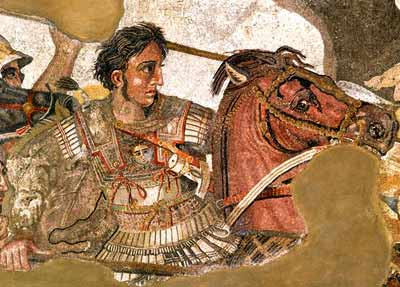
\includegraphics[width=0.6\textwidth]{alexander-great-mosaic.jpg}\end{figure}
{\em In 335 B.C., Alexander the Great began his campaign to recapture former Greek cities and to expand his empire. After ten years of undefeated battles, Alexander controlled an empire that included Greece, Egypt, and what had been the massive Persian Empire.

That wasn't enough for Xander. He decided to continue his conquest into India. But after ten years of fighting and being away from home, his men lacked the will to take part in another battle, especially against an opponent like King Porus and his army. Alexander used the talent for oration he had developed while studying under Aristotle to infuse his men with the motivation they needed to continue on, to fight and to win.}

\vspace{10 mm}

I observe, gentlemen, that when I would lead you on a new venture you no longer follow me with your old spirit. I have asked you to meet me that we may come to a decision together: are we, upon my advice, to go forward, or, upon yours, to turn back?

If you have any complaint to make about the results of your efforts hitherto, or about myself as your commander, there is no more to say. But let me remind you: through your courage and endurance you have gained possession of Ionia, the Hellespont, both Phrygias, Cappadocia, Paphlagonia, Lydia, Caria, Lycia, Pamphylia, Phoenicia, and Egypt; the Greek part of Libya is now yours, together with much of Arabia, lowland Syria, Mesopotamia, Babylon, and Susia; Persia and Media with all the territories either formerly controlled by them or not are in your hands; you have made yourselves masters of the lands beyond the Caspian Gates, beyond the Caucasus, beyond the Tanais, of Bactria, Hyrcania, and the Hyrcanian sea; we have driven the Scythians back into the desert; and Indus and Hydaspes, Acesines and Hydraotes flow now through country which is ours. With all that accomplished, why do you hesitate to extend the power of Macedon--your power--to the Hyphasis and the tribes on the other side ? Are you afraid that a few natives who may still be left will offer opposition? Come, come! These natives either surrender without a blow or are caught on the run--or leave their country undefended for your taking; and when we take it, we make a present of it to those who have joined us of their own free will and fight on our side.

For a man who is a man, work, in my belief, if it is directed to noble ends, has no object beyond itself; none the less, if any of you wish to know what limit may be set to this particular camapaign, let me tell you that the area of country still ahead of us, from here to the Ganges and the Eastern ocean, is comparatively small. You will undoubtedly find that this ocean is connected with the Hyrcanian Sea, for the great Stream of Ocean encircles the earth. Moreover I shall prove to you, my friends, that the Indian and Persian Gulfs and the Hyrcanian Sea are all three connected and continuous. Our ships will sail round from the Persian Gulf to Libya as far as the Pillars of Hercules, whence all Libya to the eastward will soon be ours, and all Asia too, and to this empire there will be no boundaries but what God Himself has made for the whole world.

But if you turn back now, there will remain unconquered many warlike peoples between the Hyphasis and the Eastern Ocean, and many more to the northward and the Hyrcanian Sea, with the Scythians, too, not far away; so that if we withdraw now there is a danger that the territory which we do not yet securely hold may be stirred to revolt by some nation or other we have not yet forced into submission. Should that happen, all that we have done and suffered will have proved fruitless--or we shall be faced with the task of doing it over again from the beginning. Gentlemen of Macedon, and you, my friends and allies, this must not be. Stand firm; for well you know that hardship and danger are the price of glory, and that sweet is the savour of a life of courage and of deathless renown beyond the grave.

Are you not aware that if Heracles, my ancestor, had gone no further than Tiryns or Argos--or even than the Peloponnese or Thebes--he could never have won the glory which changed him from a man into a god, actual or apparent? Even Dionysus, who is a god indeed, in a sense beyond what is applicable to Heracles, faced not a few laborious tasks; yet we have done more: we have passed beyond Nysa and we have taken the rock of Aornos which Heracles himself could not take. Come, then; add the rest of Asia to what you already possess--a small addition to the great sum of your conquests. What great or noble work could we ourselves have achieved had we thought it enough, living at ease in Macedon, merely to guard our homes, accepting no burden beyond checking the encroachment of the Thracians on our borders, or the Illyrians and Triballians, or perhaps such Greeks as might prove a menace to our comfort ?

I could not have blamed you for being the first to lose heart if I, your commander, had not shared in your exhausting marches and your perilous campaigns; it would have been natural enough if you had done all the work merely for others to reap the reward. But it is not so. You and I, gentlemen, have shared the labour and shared the danger, and the rewards are for us all. The conquered territory belongs to you; from your ranks the governors of it are chosen; already the greater part of its treasure passes into your hands, and when all Asia is overrun, then indeed I will go further than the mere satisfaction of our ambitions: the utmost hopes of riches or power which each one of you cherishes will be far surpassed, and whoever wishes to return home will be allowed to go, either with me or without me. I will make those who stay the envy of those who return.


\chapter{Marcus Tullius Cicero - The First Oration Against Catiline}

\textbf{\Large{Rome -- 63 B.C.}}

\vspace{10 mm}

\begin{figure}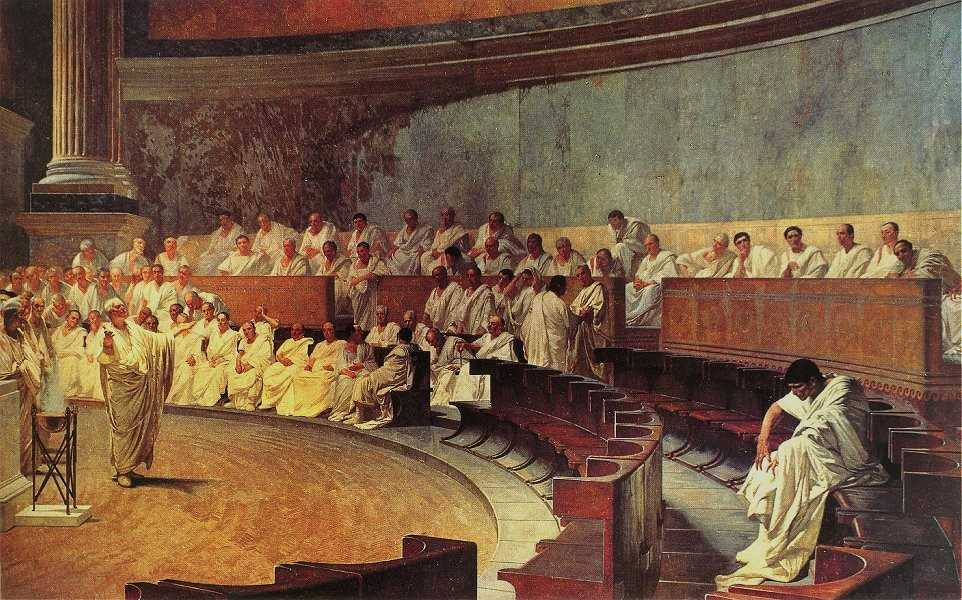
\includegraphics[width=0.6\textwidth]{catiline.jpg}\end{figure}
{\em Lucius Sergius Catilina (Catiline to his friends) was a very jealous man. Having once run against Cicero for the position of consul and lost, he became determined to win the next election by any devious method necessary. Plan A was to bribe people to vote for him, and when that didn't work, he decided to go for bust and simply knock Cicero off on election day. This plan was ferreted out by the ever vigilant Cicero, the election was postponed, and the Senate established marital law. When the election finally was held, the murderer-cum-candidate was surprisingly trounced at the polls. Now it was time for Catiline's Plan C: raise an army of co-conspirators, create insurrection throughout Italy, overthrow the government, and slice and dice as many Senators as they could get their coo-ky hands on. But Cicero was again one step ahead and discovered the plan. He called the Senate together for a meeting at the Temple of Jupiter in the Capitol, an orifice only used in times of great crisis. Catiline, who seriously didn't know when he was not welcome, decided to crash the party. With his archenemy in attendance, Cicero began his Catiline Orations, a series of speeches covering how he saved Rome from rebellion, the guilt of Catiline, and the need to whack he and his cronies.}

\vspace{10 mm}

When,  O Catiline, do you mean to cease abusing our patience? How long is that madness of yours still to mock us? When is there to be an end of that unbridled audacity of yours, swaggering about as it does now? Do not the nightly guards placed on the Palatine Hill—do not the watches posted throughout the city—does not the alarm of the people, and the union of all good men—does not the precaution taken of assembling the senate in this most defensible place—do not the looks and countenances of this venerable body here present, have any effect upon you? Do you not feel that your plans are detected? Do you not see that your conspiracy is already arrested and rendered powerless by the knowledge which every one here possesses of it? What is there that you did last night, what the night before—where is it that you were—who was there that you summoned to meet you—what design was there which was adopted by you, with which you think that any one of us is unacquainted?

Shame on the age and on its principles! The senate is aware of these things; the consul sees them; and yet this man lives. Lives! aye, he comes even into the senate. He takes a part in the public deliberations; he is watching and marking down and checking off for slaughter every individual among us. And we, gallant men that we are, think that we are doing our duty to the republic if we keep out of the way of his frenzied attacks.

You ought, O Catiline, long ago to have been led to execution by command of the consul. That destruction which you have been long plotting against us ought to have already fallen on your own head.	 3

What? Did not that most illustrious man, Publius Scipio, the Pontifex Maximus, in his capacity of a private citizen, put to death Tiberius Gracchus, tho but slightly undermining the constitution? And shall we, who are the consuls, tolerate Catiline, openly desirous to destroy the whole world with fire and slaughter? For I pass over older instances, such as how Caius Servilius Ahala with his own hand slew Spurius Malius when plotting a revolution in the state. There was—there was once such virtue in this republic that brave men would repress mischievous citizens with severer chastisement than the most bitter enemy. For we have a resolution of the senate, a formidable and authoritative decree against you, O Catiline; the wisdom of the republic is not at fault, nor the dignity of this senatorial body. We, we alone—I say it openly,—we, the consuls, are wanting in our duty.

The senate once passed a decree that Lucius Opimius, the consul, should take care that the republic suffered no injury. Not one night elapsed. There was put to death, on some mere suspicion of disaffection, Caius Gracchus, a man whose family had borne the most unblemished reputation for many generations. There was slain Marcus Fulvius, a man of consular rank, and all his children. By a like decree of the senate the safety of the republic was entrusted to Caius Marius and Lucius Valerius, the consuls. Did not the vengeance of the republic, did not execution overtake Lucius Saturninus, a tribune of the people, and Caius Servilius, the pretor, without the delay of one single day? But we, for these twenty days, have been allowing the edge of the senate's authority to grow blunt, as it were. For we are in possession of a similar decree of the senate, but we keep it locked up in its parchment—buried, I may say, in the sheath; and according to this decree you ought, O Catiline, to be put to death this instant. You live,—and you live, not to lay aside, but to persist in your audacity.

I wish, O conscript fathers, to be merciful; I wish not to appear negligent amid such danger to the state; but I do now accuse myself of remissness and culpable inactivity. A camp is pitched in Italy, at the entrance of Etruria, in hostility to the republic; the number of the enemy increases every day; and yet the general of that camp, the leader of those enemies, we see within the walls—aye, and even in the senate—planning every day some internal injury to the republic. If, O Catiline, I should now order you to be arrested, to be put to death, I should, I suppose, have to fear lest all good men should say that I had acted tardily, rather than that any one should affirm that I acted cruelly. But yet this, which ought to have been done long since, I have good reason for not doing as yet; I will put you to death, then, when there shall be not one person possible to be found so wicked, so abandoned, so like yourself, as not to allow that it has been rightly done. As long as one person exists who can dare to defend you, you shall live; but you shall live as you do now, surrounded by my many and trusty guards, so that you shall not be able to stir one finger against the republic; many eyes and ears shall still observe and watch you, as they have hitherto done, tho you shall not perceive them.

For what is there, O Catiline, that you can still expect, if night is not able to veil your nefarious meetings in darkness, and if private houses can not conceal the voice of your conspiracy within their walls—if everything is seen and displayed? Change your mind: trust me: forget the slaughter and conflagration you are meditating. You are hemmed in on all sides; all your plans are clearer than the day to us; let me remind you of them. Do you recollect that on the 21st of October I said in the senate that on a certain day, which was to be the 27th of October, C. Manlius, the satellite and servant of your audacity, would be in arms? Was I mistaken, Catiline, not only in so important, so atrocious, so incredible a fact, but, what is much more remarkable, in the very day? I said also in the senate that you had fixed the massacre of the nobles for the 28th of October when many chief men of the senate had left Rome, not so much for the sake of saving themselves as of checking your designs. Can you deny that on that very day you were so hemmed in by my guards and my vigilance that you were unable to stir one finger against the republic; when you said that you would be content with the flight of the rest, and the slaughter of us who remained? What? when you made sure that you would be able to seize Praneste on the 1st of November by a nocturnal attack, did you not find that that colony was fortified by my order, by my garrison, by my watchfulness and care? You do nothing, you plan nothing, you think of nothing which I not only do not hear, but which I do not see and know every particular of.

Listen while I speak of the night before. You shall now see that I watch far more actively for the safety than you do for the destruction of the republic. I say that you came the night before (I will say nothing obscurely) into the Scythedealers' Street, to the house of Marcus Lecca; that many of your accomplices in the same insanity and wickedness came there, too. Do you dare to deny it? Why are you silent? I will prove it if you do deny it; for I see here in the senate some men who were there with you.

O ye immortal gods, where on earth are we? in what city are we living? what constitution is ours? There are here,—here in our body, O conscript fathers, in this the most holy and dignified assembly of the whole world, men who meditate my death, and the death of all of us, and the destruction of this city, and of the whole world. I, the consul, see them; I ask them their opinion about the republic, and I do not yet attack, even by words, those who ought to be put to death by the sword. You were, then, O Catiline, at Lecca's that night; you divided Italy into sections; you settled where every one was to go; you fixed whom you were to leave at Rome, whom you were to take with you; you portioned out the divisions of the city for conflagration; you undertook that you yourself would at once leave the city, and said that there was then only this to delay you,—that I was still alive. Two Roman knights were found to deliver you from this anxiety, and to promise that very night, before daybreak, to slay me in my bed. All this I knew almost before your meeting had broken up. I strengthened and fortified my house with a stronger guard; I refused admittance, when they came, to those whom you sent in the morning to salute me, and of whom I had foretold to many eminent men that they would come to me at that time.

As, then, this is the case, O Catiline, continue as you have begun. Leave the city at least; the gates are open; depart. That Manlian camp of yours has been waiting too long for you as its general. And lead forth with you all your friends, or at least as many as you can; purge the city of your presence; you will deliver me from a great fear, when there is a wall between you and me. Among us you can dwell no longer—I will not bear it, I will not permit it, I will not tolerate it. Great thanks are due to the immortal gods, and to this very Jupiter Stator, in whose temple we are, the most ancient protector of this city, that we have already so often escaped so foul, so horrible, and so deadly an enemy to the republic. But the safety of the commonwealth must not be too often allowed to be risked on one man. As long as you, O Catiline, plotted against me while I was the consul-elect, I defended myself, not with a public guard, but by my own private diligence. When, in the next consular comitia, you wished to slay me when I was actually consul, and your competitors also, in the Campus Martius, I checked your nefarious attempt by the assistance and resources of my own friends, without exciting any disturbance publicly. In short, as often as you attacked me, I by myself opposed you, and that, too, tho I saw that my ruin was connected with great disaster to the republic. But now you are openly attacking the entire republic.

You are summoning to destruction and devastation the temples of the immortal gods, the houses of the city, the lives of all the citizens—in short, all Italy. Wherefore, since I do not yet venture to do that which is the best thing, and which belongs to my office and to the discipline of our ancestors, I will do that which is more merciful if we regard its rigor, and more expedient for the State. For if I order you to be put to death, the rest of the conspirators will still remain in the republic; if, as I have long been exhorting you, you depart, your companions, those worthless dregs of the republic, will be drawn off from the city, too. What is the matter, Catiline? Do you hesitate to do that when I order you which you were already doing of your own accord? The consul orders an enemy to depart from the city. Do you ask me, Are you to go into banishment? I do not order it; but, if you consult me, I advise it.

For what is there, O Catiline, that can now afford you any pleasure in this city? for there is no one in it, except that band of profligate conspirators of yours, who does not fear you,—no one who does not hate you. What brand of domestic baseness is not stamped upon your life? What disgraceful circumstance is wanting to your infamy in your private affairs? From what licentiousness have your eyes, from what atrocity have your hands, from what iniquity has your whole body ever abstained? Is there one youth, when you have once entangled him in the temptations of your corruption, to whom you have not held out a sword for audacious crime, or a torch for licentious wickedness?

What? when lately by the death of your former wife you had made your house empty and ready for a new bridal, did you not even add another incredible wickedness to this wickedness? But I pass that over, and willingly allow it to be buried in silence, that so horrible a crime may not be seen to have existed in this city, and not to have been chastised. I pass over the ruin of your fortune, which you know is hanging over you against the ides of the very next month; I come to those things which relate not to the infamy of your private vices, not to your domestic difficulties and baseness, but to the welfare of the republic and to the lives and safety of us all.

Can the light of this life, O Catiline, can the breath of this atmosphere be pleasant to you, when you know that there is not one man of those here present who is ignorant that you, on the last day of the year, when Lepidus and Tullus were consuls, stood in the assembly armed; that you had prepared your hand for the slaughter of the consuls and chief men of the state, and that no reason or fear of yours hindered your crime and madness, but the fortune of the republic? And I say no more of these things, for the are not unknown to every one. How often have you endeavored to slay me, both as consul-elect and as actual consul? How many shots of yours, so aimed that they seemed impossible to be escaped, have I avoided by some slight stooping aside, and some dodging, as it were, of my body? You attempt nothing, you execute nothing, you devise nothing that can be kept hid from me at the proper time; and yet you do not cease to attempt and to contrive. How often already has that dagger of yours been wrested from your hands? How often has it slipped through them by some chance, and dropped down? And yet you can not any longer do without it; and to what sacred mysteries it is consecrated and devoted by you I know not, that you think it necessary to plunge it in the body of the consul.

But now, what is that life of yours that you are leading? For I will speak to you not so as to seem influenced by the hatred I ought to feel, but by pity, nothing of which is due to you. You came a little while ago into the senate; in so numerous an assembly, who of so many friends and connections of yours saluted you? If this in the memory of man never happened to any one else, are you waiting for insults by word of mouth, when you are overwhelmed by the most irresistible condemnation of silence? Is it nothing that at your arrival all those seats were vacated? that all the men of consular rank, who had often been marked out by you for slaughter, the very moment you sat down, left that part of the benches bare and vacant? With what feelings do you think you ought to bear this? On my honor, if my slaves feared me as all your fellow citizens fear you, I should think I must leave my house. Do not you think you should leave the city? If I say that I was even undeservedly so suspected and hated by my fellow citizens, I would rather flee from their sight than be gazed at by the hostile eyes of every one. And do you, who, from the consciousness of your wickedness, know that the hatred of all men is just and has been long due to you, hesitate to avoid the sight and presence of those men whose minds and senses you offend? If your parents feared and hated you, and if you could by no means pacify them, you would, I think, depart somewhere out of their sight. Now, your country, which is the common parent of all of us, hates and fears you, and has no other opinion of you, than that you are meditating parricide in her case; and will you neither feel awe of her authority, nor deference for her judgment, nor fear of her power?

And she, O Catiline, thus pleads with you, and after a manner silently speaks to you: There has now for many years been no crime committed but by you; no atrocity has taken place without you; you alone unpunished and unquestioned have murdered the citizens, have harassed and plundered the allies; you alone have had power not only to neglect all laws and investigations, but to overthrow and break through them. Your former actions, tho they ought not to have been borne, yet I did bear as well as I could; but now that I should be wholly occupied with fear of you alone, that at every sound I should dread Catiline, that no design should seem possible to be entertained against me which does not proceed from your wickedness, this is no longer endurable. Depart, then, and deliver me from this fear—that, if it be a just one, I may not be destroyed; if an imaginary one, that at least I may at last cease to fear.

If, as I have said, your country were thus to address you, ought she not to obtain her request, even if she were not able to enforce it? What shall I say of your having given yourself into custody? what of your having said, for the sake of avoiding suspicion, that you were willing to dwell in the house of Marcus Lepidus? And when you were not received by him, you dared even to come to me, and begged me to keep you in my house; and when you had received answer from me that I could not possibly be safe in the same house with you, when I considered myself in great danger as long as we were in the same city, you came to Quintus Metellus, the pretor, and being rejected by him, you passed on to your associate, that most excellent man, Marcus Marcellus, who would be, I suppose you thought, most diligent in guarding you, most sagacious in suspecting you, and most bold in punishing you; but how far can we think that man ought to be from bonds and imprisonment who has already judged himself deserving of being given into custody.

Since, then, this is the case, do you hesitate, O Catiline, if you can not remain here with tranquillity, to depart to some distant land, and to trust your life, saved from just and deserved punishment, to flight and solitude? Make a motion, say you, to the senate (for that is what you demand), and if this body votes that you ought to go into banishment, you say that you will obey. I will not make such a motion—it is contrary to my principles, and yet I will let you see what these men think of you. Be gone from the city, O Catiline; deliver the republic from fear; depart into banishment, if that is the word you are waiting for. What now, O Catiline? Do you not perceive, do you not see the silence of these men; they permit it, they say nothing; why wait you for the authority of their words when you see their wishes in their silence?

But had I said the same to this excellent young man, Publius Sextius, or to that brave man, Marcus Marcellus, before this time the senate would deservedly have laid violent hands on me, consul tho I be, in this very temple. But as to you, Catiline, while they are quiet they approve, while they permit me to speak they vote, while they are silent they are loud and eloquent. And not they alone, whose authority forsooth is dear to you, tho their lives are unimportant, but the Roman knights, too, those most honorable and excellent men, and the other virtuous citizens who are now surrounding the senate, whose numbers you could see, whose desires you could know, and whose voices you a few minutes ago could hear,—aye, whose very hands and weapons I have for some time been scarcely able to keep off from you; but those, too, I will easily bring to attend you to the gates if you leave these places you have been long desiring to lay waste.

And yet, why am I speaking? That anything may change your purpose? that you may ever amend your life? that you may meditate flight or think of voluntary banishment? I wish the gods may give you such a mind; tho I see, if alarmed at my words you bring your mind to go into banishment, what a storm of unpopularity hangs over me, if not at present, while the memory of your wickedness is fresh, at all events hereafter. But it is worth while to incur that, as long as that is but a private misfortune of my own, and is unconnected with the dangers of the republic. But we can not expect that you should be concerned at your own vices, that you should fear the penalties of the laws, or that you should yield to the necessities of the republic, for you are not, O Catiline, one whom either shame can recall from infamy, or fear from danger, or reason from madness.

Wherefore, as I have said before, go forth, and if you wish to make me, your enemy as you call me, unpopular, go straight into banishment. I shall scarcely be able to endure all that will be said if you do so; I shall scarcely be able to support my load of unpopularity if you do go into banishment at the command of the consul; but if you wish to serve my credit and reputation, go forth with your ill-omened band of profligates; betake yourself to Manlius, rouse up the abandoned citizens, separate yourself from the good ones, wage war against your country, exult in your impious banditti, so that you may not seem to have been driven out by me and gone to strangers, but to have gone invited to your own friends.

Tho why should I invite you, by whom I know men have been already sent on to wait in arms for you at the forum Aurelium; who I know has fixed and agreed with Manlius upon a settled day; by whom I know that that silver eagle, which I trust will be ruinous and fatal to you and to all your friends, and to which there was set up in your house a shrine as it were of your crimes, has been already sent forward. Need I fear that you can long do without that which you used to worship when going out to murder, and from whose altars you have often transferred your impious hand to the slaughter of citizens?

You will go at last where your unbridled and mad desire has been long hurrying you. And this causes you no grief, but an incredible pleasure. Nature has formed you, desire has trained you, fortune has preserved you for this insanity. Not only did you never desire quiet, but you never even desired any war but a criminal one; you have collected a band of profligates and worthless men, abandoned not only by all fortune but even by hope.

Then what happiness will you enjoy! with what delight will you exult! in what pleasure will you revel! when in so numerous a body of friends, you neither hear nor see one good man. All the toils you have gone through have always pointed to this sort of life; your lying on the ground not merely to lie in wait to gratify your unclean desires, but even to accomplish crimes; your vigilance, not only when plotting against the sleep of husbands, but also against the goods of your murdered victims, have all been preparations for this. Now you have an opportunity of displaying your splendid endurance of hunger, of cold, of want of everything; by which in a short time you will find yourself worn out. All this I effected when I procured your rejection from the consulship, that you should be reduced to make attempts on your country as an exile, instead of being able to distress it as consul, and that that which had been wickedly undertaken by you should be called piracy rather than war.

Now that I may remove and avert, O conscript fathers, any in the least reasonable complaint from myself, listen, I beseech you, carefully to what I say, and lay it up in your inmost hearts and minds. In truth, if my country, which is far dearer to me than my life—if all Italy—if the whole republic were to address me, “Marcus Tullius, what are you doing? will you permit that man to depart whom you have ascertained to be an enemy? whom you see ready to become the general of the war? whom you know to be expected in the camp of the enemy as their chief, the author of all this wickedness, the head of the conspiracy, the instigator of the slaves and abandoned citizens, so that he shall seem not driven out of the city by you, but let loose by you against the city? Will you not order him to be thrown into prison, to be hurried off to execution, to be put to death with the most prompt severity? What hinders you? Is it the customs of our ancestors? But even private men have often in this republic slain mischievous citizens. Is it the laws which have been passed about the punishment of Roman citizens? But in this city those who have rebelled against the republic have never had the rights of citizens. Do you fear odium with posterity? You are showing fine gratitude to the Roman people which has raised you, a man known only by your own actions, of no ancestral renown, through all the degrees of honor at so early an age to the very highest office, if from fear of unpopularity or of any danger you neglect the safety of your fellow citizens. But if you have a fear of unpopularity, is that arising from the imputation of vigor and boldness, or that arising from that of inactivity and indecision most to be feared? When Italy is laid waste by war, when cities are attacked and houses in flames, do you not think that you will be then consumed by a perfect conflagration of hatred?

To this holy address of the republic, and to the feelings of those men who entertain the same opinion, I will make this short answer: If, O conscript fathers, I thought it best that Catiline should be punished with death, I would not have given the space of one hour to this gladiator to live in. If, forsooth, those excellent men and most illustrious cities not only did not pollute themselves, but even glorified themselves by the blood of Saturninus, and the Gracchi, and Flaccus, and many others of old time, surely I had no cause to fear lest for slaying this parricidal murderer of the citizens any unpopularity should accrue to me with posterity. And if it did threaten me to ever so great a degree, yet I have always been of the disposition to think unpopularity earned by virtue and glory not unpopularity.

Tho there are some men in this body who either do not see what threatens, or dissemble what they do see; who have fed the hope of Catiline by mild sentiments, and have strengthened the rising conspiracy by not believing it; influenced by whose authority many, and they not wicked, but only ignorant, if I punished him would say that I had acted cruelly and tyrannically. But I know that if he arrives at the camp of Manlius to which he is going, there will be no one so stupid as not to see that there has been a conspiracy, no one so hardened as not to confess it. But if this man alone were put to death, I know that this disease of the republic would be only checked for a while, not eradicated forever. But if he banishes himself, and takes with him all his friends, and collects at one point all the ruined men from every quarter, then not only will this full-grown plague of the republic be extinguished and eradicated, but also the root and seed of all future evils.

We have now for a long time, O conscript fathers, lived among these dangers and machinations of conspiracy; but somehow or other, the ripeness of all wickedness, and of this long-standing madness and audacity, has come to a head at the time of my consulship. But if this man alone is removed from this piratical crew, we may appear, perhaps, for a short time relieved from fear and anxiety, but the danger will settle down and lie hid in the veins and bowels of the republic. As it often happens that men afflicted with a severe disease, when they are tortured with heat and fever, if they drink cold water, seem at first to be relieved, but afterward suffer more and more severely; so this disease which is in the republic, if relieved by the punishment of this man, will only get worse and worse, as the rest will be still alive.

Wherefore, O conscript fathers, let the worthless be gone,—let them separate themselves from the good,—let them collect in one place,—let them, as I have often said before, be separated from us by a wall; let them cease to plot against the consul in his own house,—to surround the tribunal of the city pretor,—to besiege the senate-house with swords,—to prepare brands and torches to burn the city; let it, in short, be written on the brow of every citizen, what his sentiments are about the republic. I promise you, this, O conscript fathers, that there shall be so much diligence in us the consuls, so much authority in you, so much virtue in the Roman knights, so much unanimity in all good men that you shall see everything made plain and manifest by the departure of Catiline,—everything checked and punished.

With these omens, O Catiline, be gone to your impious and nefarious war, to the great safety of the republic, to your own misfortune and injury, and to the destruction of those who have joined themselves to you in every wickedness and atrocity. Then do you, O Jupiter, who were consecrated by Romulus with the same auspices as this city, whom we rightly call the stay of this city and empire, repel this man and his companions from your altars and from the other temples,—from the houses and walls of the city,—from the lives and fortunes of all the citizens; and overwhelm all the enemies of good men, the foes of the republic, the robbers of Italy, men bound together by a treaty and infamous alliance of crimes, dead and alive, with eternal punishments.


\chapter{Jesus Christ - Sermon on the Mount}

\textbf{\Large{Jerusalem -- 33 }}

\vspace{10 mm}

\begin{figure}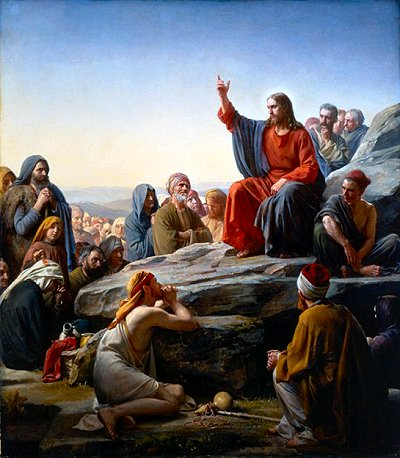
\includegraphics[width=0.6\textwidth]{sermon-on-the-mount.jpg}\end{figure}
{\em Whether one believes that Jesus of Nazareth was the Son of God or simply a wise teacher, it is impossible to deny the impact of perhaps the world's most famous speech: The Sermon on the Mount. No speech has been more pondered, more influential, or more quoted. It introduced a prayer now familiar the world over and uttered in trenches, churches, and bedsides around the globe. It introduced a code of conduct billions of believers have adopted as their lofty, if not not always attainable, goal. While much of the sermon has roots in Jewish law, the advice given in the Beatitudes represented a dramatic and radical departure from the eye for an eye system of justice known in the ancient world. The standards of behavior outlined in the sermon have given believers and non-believers alike plenty to contemplate and discuss in the two thousand years since it was given.}

\vspace{10 mm}

Blessed are those who recognize they are spiritually poor, for the kingdom of heaven is theirs. Blessed are those who grieve, for they shall be consoled. Blessed are those who are kind, for they will be given the world. Blessed are those who are hungry and thirsty for what is right, for they will be filled up. Blessed are those who are merciful, for they will be shown mercy. Blessed are the pure-hearted, for they will see God. Blessed are those who make peace, because they will be called children of God. Blessed are those who have been persecuted for the right, because the kingdom of heaven belongs to them. Blessed are you when people insult you and persecute you and tell all kind of evil lies against you because of me. Celebrate and be happy for your compensation in heaven will be great, for in the same way they persecuted the prophets who were before you.

You're the earth's salt, but if the salt becomes tasteless, what can you make salty with it? It's useless, and is tossed out where people walk on it. You're the world's light. A city built on a hull can't be hidden. People don't light a lamp and put it under a bucket. Instead they put it on a lamp-stand and it gives light to everyone in the house. In the same way let your light shine in front of people so they can see the good things you do and praise your heavenly Father.

Don't think I came to abolish the law or the prophets' writings. I didn't come to abolish them, but to fulfill them. I promise you, until heaven and earth are gone, not one hyphen nor one dot will be gone from the law before everything is fulfilled. So whoever breaks the least important commandment, and teaches people to do so, will be called the least in the kingdom of heaven; but whoever practices and teaches them will be called great in the kingdom of heaven. I tell you, unless your righteousness is better than that of the religious teachers and the Pharisees, there's no way you'll enter the kingdom of heaven.

You've heard what was said to the people of long ago, ‘You shall not kill, and anyone who kills will be judged as guilty.' But I tell you, anyone who's furious with his brother is judged as guilty, and whoever calls his brother an idiot is liable to the Sanhedrin council, and whoever curses people with insults is liable to the fire of punishment.[]

So if you're at the altar making an offering, and remember that your brother has something against you, leave your offering on the altar and go and make peace with him first, and afterward come back and make your offering. Agree with your opponent quickly while you're with him on the way to court, so that he doesn't hand you over to the judge, and the judge hand you over to the officer and you're thrown into jail. I tell you the truth, you won't get out of there until you've paid the last penny.

You've heard it said, ‘Do not commit adultery.' But I tell you that everyone who looks at a married woman[] covetously[] has already committed adultery with her in his heart. If your right eye leads you to sin, then tear it out and throw it away, because it's better to lose one of part of your than to have the whole of your body thrown into hell.[] And if your right hand leads you to sin, then cut it off, and throw it away, because it's better for you to lose one of your limbs than to for your whole body to go into hell.

It was also said, ‘Whoever divorces his wife, let him give her a certificate of divorce.' But I tell you that everyone who divorces his wife except for sexual immorality causes her to commit adultery and whoever married a divorcee commits adultery.

And again, you've heard what was said to the people of long ago, You shall not perjure yourself, instead keep the oaths you make to the Lord. But I tell you, don't swear at all, not by heaven, because it's the throne of God, not by the earth, because it's God's footstool, not by Jerusalem, because it's the city of the great King. Don't even swear by your head, because you're not able to make one hair white or black. Simply say yes, or no—more than this comes from the evil one.

You've heard that it was said, ‘An eye in place of an eye, and a tooth in place of a tooth.' But I tell you, don't oppose someone who is evil. Whoever slaps you on the right cheek, turn the other cheek to him as well; and to whoever wants to get a judgment against you and takes your shirt, give him your coat too; and if someone forces you to go one mile, go with him two. Give to whoever asks you, and lend to whoever wants to borrow from you—don't turn them away.

You've heard that it was said, Love your neighbor and hate your enemy. But I tell you, love your enemies and pray for those who persecute you, so you may become children of your heavenly Father. For he makes his sun rise on the evil and the good; and rain to fall on those who do right and those who don't. Because if you love those who love you, what reward do you have? Don't the tax-collectors do that? And if you only speak kindly to your family, what are you doing more than anybody else? Don't even the Gentiles do that? Then you'll be perfectly mature, as your heavenly Father is perfect.

Be careful not to do your good deeds in front of people, so they can be observed—otherwise you have no reward from your Father in heaven. When you give to the poor, don't trumpet this before others like the hypocrites do in the synagogues and in the streets so that they will be praised by people. I tell you the truth: they have already got their reward. When you give to the poor, don't let your left hand know what your right hand's doing, so that your charitable giving may be secret, and your Father who sees what happens in secret will reward you.

And when you pray, don't be like the hypocrites because they love to stand up and pray in the synagogues and on the street corners so that people can see them. I promise you, they have already got their reward. But you, when you pray, go indoors and close the door, and pray to your Father in private, and your Father who sees what happens in private will reward you. When you pray, don't babble on meaninglessly like the Gentiles do, who think they will be heard because of all the words they speak. Don't be like them, because your Father knows what you need even before you ask him. So pray like this:

Our Father in heaven, may your name be revered. May your kingdom come. May your will be carried out in earth as in heaven. Please give to us today the bread we need to live each day. Forgive us our sins, as we have forgiven those who sinned against us. Don't bring us into temptation, and rescue us from the evil one.

For if you forgive those who sin against you, your heavenly Father will also forgive you. But if you don't forgive those who sin against you, then your heavenly Father won't forgive your sins.

And when you fast, don't be like the hypocrites who put on sad faces and make themselves look horrible so that they can make it obvious to people they're fasting. But you, when you fast, wash your face and look smart, so that people won't see you're fasting, and your Father who sees what happens in private will reward you.

Don't store up wealth for yourselves here on earth where moth and rust ruin it, and where thieves break in and steal. Instead store up wealth for yourselves in heaven, where moth and rust don't ruin it, and where thieves don't break in and steal. For whatever you value, that's where your heart will be.

The eye is the body's lamp. So if your eye is clear, then your whole body will be lit up. But if your eye is evil, then your whole body will be in the dark. Then if the light in you is darkness, how dark is that! No one can serve two masters. Either you'll hate one and love the other, or you'll be devoted to one and despise the other. You can't serve God ad Money.

That's why I'm telling you not to worry about your life, about what to eat, or what to drink, or what clothes to put on. Isn't life more than food, and the body more than clothes? Look at the wild birds—they don't sow or reap or store food in barns, for your heavenly Father feeds them. Aren't you worth more then them? And who of you by worrying can add a minute to your life? And why are you worried about clothes? Look at the beautiful flowers in the field, how they grow—they don't work hard, they don't spin thread. But I tell you, not even Solomon in all his majesty was dressed like one of these flowers. So if God decorates the grass in the field like this, which is here today and tomorrow is thrown into the fire, won't he do much more for you, you people of little faith? So don't worry, saying, ‘What shall we eat' or ‘What shall we drink?' or ‘What shall we wear?' All these things are what the pagans run after, but your heavenly Father knows everything you need. You should look for his kingdom first, and his way of doing right, and everything will be given to you. So don't worry about tomorrow, because tomorrow can worry about itself. There's already enough that's bad in every day.

Don't judge others, and you won't be judged. For whatever standard you use to judge others will be used to judge you, and whatever measurement you use to measure others will be used to measure you. Why do you look at the speck that's in your brother's eye, and don't notice the plank that's in your own eye? How are you going to say to your brother, ‘Let me take out the speck from your eye' when you have a plank in you own eye? You hypocrite, first get rid of the plank in your own eye, and then you'll see clearly to take out the speck from your brother's eye.

Don't give what's holy to dogs, and don't throw your pearls to pigs, so that they don't trample them underfoot and then turn and gore you.

Ask, and it will be given to you, seek, and you will find, knock, and the door will be opened for you. Everyone who asks, receives; and whoever seeks, finds; and whoever knocks, the door is opened for them. Is there anyone of you who when your son asks for bread, you give him a stone? Or if he asks for fish, you give him a snake? If even you who're evil know to give good things to your children, how much more will your father in heaven give good things to those who ask him.

Whatever you want people to do to you, do to them too—this sums up the law and the prophets. Enter through the narrow entrance, for wide is the entrance, and broad the way that leads to destruction, and many go that way. But narrow is the entrance and tight the way that leads to life, and only a few find it.

Watch out for false prophets who will come in sheep's clothing, but inside are vicious wolves. Recognize them by the fruits of their actions. Do people harvest grapes from thorn-bushes, or figs from thistles? In the same way every good tree produces good fruit, but a bad tree produces bad fruit. A good tree can't produce bad fruit, nor can a bad tree produce good fruit. Every tree that doesn't produce good fruit is chopped down and thrown into the fire. So by their fruits you'll know them.

Not everyone who calls me Master, master, will enter the kingdom of heaven, rather it's those who do the will of my Father in heaven. There will be many who say to me in the day of judgment, ‘Lord, Lord, didn't we preach for you and drive out demons in your name and performed many miracles with your authority?' Then I'll declare to them, ‘I never knew you—leave me you who practice wickedness.' Everyone who hears what I say, and does what I tell them, they are like a wise man who built his house on solid rock. The rain poured down, and the floods rose, and the winds blew hard against the house, but it didn't fall down, because its foundations were on solid rock. Everyone who hears what I say, and doesn't do what I tell them, they are like a moron who built his house on the sand. The rain poured down, and the floods rose, and the winds blew hard against the house, and it fell down—it totally collapsed.


\chapter{Patrick Henry - Give Me Liberty or Give Me Death}

\textbf{\Large{Richmong, Virginia -- May 23, 1775 }}

\vspace{10 mm}

\begin{figure}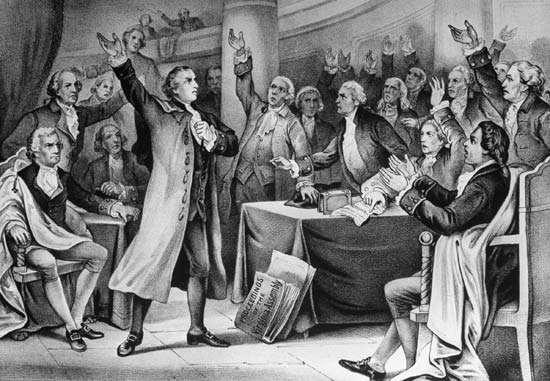
\includegraphics[width=0.6\textwidth]{henry.jpeg}\end{figure}
{\em For a decade, revolutionary sentiments had been brewing in Virginia and Patrick Henry had always been in the thick of it, stirring the pot. Henry became particularly enflamed by the Stamp Act of 1764, which prompted him to give his so-called “treason speech,” spurring the Burgesses to pass the Virginia Resolves banning the act. Tensions between the colonies and the Crown continued to build, and in 1775, Massachusetts patriots began making preparations for war. Henry believed that Virginia should follow suit. At a meeting held in St. John's Church in Richmond, Henry presented resolutions to make ready Virginia's defenses. Seeking to persuade his fellow delegates of the urgency of his message, he gave a rousing and memorable speech, climaxing is that now famous line, “Give me liberty of give me death!”}

\vspace{10 mm}

No man thinks more highly than I do of the patriotism, as well as abilities, of the very worthy gentlemen who have just addressed the House. But different men often see the same subject in different lights; and, therefore, I hope it will not be thought disrespectful to those gentlemen if, entertaining as I do opinions of a character very opposite to theirs, I shall speak forth my sentiments freely and without reserve. This is no time for ceremony. The questing before the House is one of awful moment to this country. For my own part, I consider it as nothing less than a question of freedom or slavery; and in proportion to the magnitude of the subject ought to be the freedom of the debate. It is only in this way that we can hope to arrive at truth, and fulfill the great responsibility which we hold to God and our country. Should I keep back my opinions at such a time, through fear of giving offense, I should consider myself as guilty of treason towards my country, and of an act of disloyalty toward the Majesty of Heaven, which I revere above all earthly kings.

Mr. President, it is natural to man to indulge in the illusions of hope. We are apt to shut our eyes against a painful truth, and listen to the song of that siren till she transforms us into beasts. Is this the part of wise men, engaged in a great and arduous struggle for liberty? Are we disposed to be of the number of those who, having eyes, see not, and, having ears, hear not, the things which so nearly concern their temporal salvation? For my part, whatever anguish of spirit it may cost, I am willing to know the whole truth; to know the worst, and to provide for it.

I have but one lamp by which my feet are guided, and that is the lamp of experience. I know of no way of judging of the future but by the past. And judging by the past, I wish to know what there has been in the conduct of the British ministry for the last ten years to justify those hopes with which gentlemen have been pleased to solace themselves and the House. Is it that insidious smile with which our petition has been lately received? Trust it not, sir; it will prove a snare to your feet. Suffer not yourselves to be betrayed with a kiss. Ask yourselves how this gracious reception of our petition comports with those warlike preparations which cover our waters and darken our land. Are fleets and armies necessary to a work of love and reconciliation? Have we shown ourselves so unwilling to be reconciled that force must be called in to win back our love? Let us not deceive ourselves, sir. These are the implements of war and subjugation; the last arguments to which kings resort. I ask gentlemen, sir, what means this martial array, if its purpose be not to force us to submission? Can gentlemen assign any other possible motive for it? Has Great Britain any enemy, in this quarter of the world, to call for all this accumulation of navies and armies? No, sir, she has none. They are meant for us: they can be meant for no other. They are sent over to bind and rivet upon us those chains which the British ministry have been so long forging. And what have we to oppose to them? Shall we try argument? Sir, we have been trying that for the last ten years. Have we anything new to offer upon the subject? Nothing. We have held the subject up in every light of which it is capable; but it has been all in vain. Shall we resort to entreaty and humble supplication? What terms shall we find which have not been already exhausted? Let us not, I beseech you, sir, deceive ourselves. Sir, we have done everything that could be done to avert the storm which is now coming on. We have petitioned; we have remonstrated; we have supplicated; we have prostrated ourselves before the throne, and have implored its interposition to arrest the tyrannical hands of the ministry and Parliament. Our petitions have been slighted; our remonstrances have produced additional violence and insult; our supplications have been disregarded; and we have been spurned, with contempt, from the foot of the throne! In vain, after these things, may we indulge the fond hope of peace and reconciliation. There is no longer any room for hope. If we wish to be free– if we mean to preserve inviolate those inestimable privileges for which we have been so long contending–if we mean not basely to abandon the noble struggle in which we have been so long engaged, and which we have pledged ourselves never to abandon until the glorious object of our contest shall be obtained–we must fight! I repeat it, sir, we must fight! An appeal to arms and to the God of hosts is all that is left us!

They tell us, sir, that we are weak; unable to cope with so formidable an adversary. But when shall we be stronger? Will it be the next week, or the next year? Will it be when we are totally disarmed, and when a British guard shall be stationed in every house? Shall we gather strength by irresolution and inaction? Shall we acquire the means of effectual resistance by lying supinely on our backs and hugging the delusive phantom of hope, until our enemies shall have bound us hand and foot? Sir, we are not weak if we make a proper use of those means which the God of nature hath placed in our power. The millions of people, armed in the holy cause of liberty, and in such a country as that which we possess, are invincible by any force which our enemy can send against us. Besides, sir, we shall not fight our battles alone. There is a just God who presides over the destinies of nations, and who will raise up friends to fight our battles for us. The battle, sir, is not to the strong alone; it is to the vigilant, the active, the brave. Besides, sir, we have no election. If we were base enough to desire it, it is now too late to retire from the contest. There is no retreat but in submission and slavery! Our chains are forged! Their clanking may be heard on the plains of Boston! The war is inevitable–and let it come! I repeat it, sir, let it come.

It is in vain, sir, to extenuate the matter. Gentlemen may cry, Peace, Peace– but there is no peace. The war is actually begun! The next gale that sweeps from the north will bring to our ears the clash of resounding arms! Our brethren are already in the field! Why stand we here idle? What is it that gentlemen wish? What would they have? Is life so dear, or peace so sweet, as to be purchased at the price of chains and slavery? Forbid it, Almighty God! I know not what course others may take; but as for me, give me liberty or give me death!


\chapter{George Washington - Resignation Speech}

\textbf{\Large{Washington D.C. -- December 23, 1784 }}

\vspace{10 mm}

\begin{figure}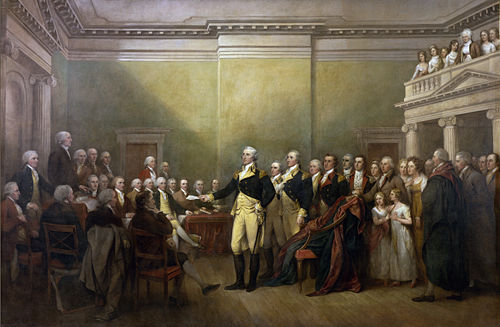
\includegraphics[width=0.6\textwidth]{500px-general_george_washington_resigning_his_commission.jpg}\end{figure}
{\em As the Revolutionary War drew to a close, there was much speculation that George Washington, then Major General and Commander-in-Chief, would follow in the footsteps of former world leaders by making a grab for supreme power. Some even wished he would do so, hoping he would become the king of a new nation. Yet Washington knew that such a move would wither the fragile beginnings of the new republic. Looking to the Roman general Cincinnatus an exemplar, Washington rejected the temptations of power and resigned his position as Commander-in-Chief. Choosing the right is almost never easy, and as Washington read his speech in front of the Continental Congress, the great statesman trembled so much that he had to hold the parchment with two hands to keep it steady. “The spectators all wept, and there was hardly a member of Congress who did not drop tears. His voice faltered and sunk, and the whole house felt his agitations.” When finished, Washington bolted from the door of the Annapolis State House, mounted his horse, and galloped away into the sunset.}

\vspace{10 mm}

The great events on which my resignation depended having at length taken place; I have now the honor of offering my sincere Congratulations to Congress and of presenting myself before them to surrender into their hands the trust committed to me, and to claim the indulgence of retiring from the Service of my Country.

Happy in the confirmation of our Independence and Sovereignty, and pleased with the opportunity afforded the United States of becoming a respectable Nation, I resign with satisfaction the Appointment I accepted with diffidence. A diffidence in my abilities to accomplish so arduous a task, which however was superseded by a confidence in the rectitude of our Cause, the support of the Supreme Power of the Union, and the patronage of Heaven.

The Successful termination of the War has verified the most sanguine expectations, and my gratitude for the interposition of Providence, and the assistance I have received from my Countrymen, increases with every review of the momentous Contest.

While I repeat my obligations to the Army in general, I should do injustice to my own feelings not to acknowledge in this place the peculiar Services and distinguished merits of the Gentlemen who have been attached to my person during the War. It was impossible the choice of confidential Officers to compose my family should have been more fortunate. Permit me Sir, to recommend in particular those, who have continued in Service to the present moment, as worthy of the favorable notice and patronage of Congress.

I consider it an indispensable duty to close this last solemn act of my Official life, by commending the Interests of our dearest Country to the protection of Almighty God, and those who have the superintendence of them, to his holy keeping.

Having now finished the work assigned me, I retire from the great theatre of Action; and bidding an Affectionate farewell to this August body under whose orders I have so long acted, I here offer my Commission, and take my leave of all the employments of public life.


\chapter{William Wilberforce - Abolition Speech}

\textbf{\Large{House of Commons, London -- May 12, 1789 }}

\vspace{10 mm}

\begin{figure}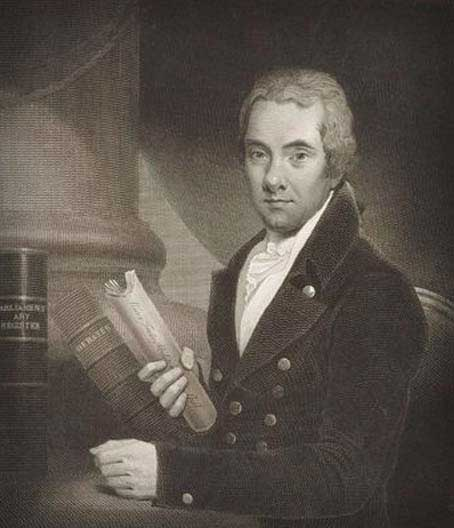
\includegraphics[width=0.6\textwidth]{williamwilberforce.jpg}\end{figure}
{\em When William Wilberforce, a member of the British Parliament, converted to Christianity, he began to earnestly seek to reform the evils he found within himself and the world around him. One of the glaring moral issues of the day was slavery, and after reading up on the subject and meeting with anti-slavery activists, Wilberforce became convinced that God was calling him to be an abolitionist. Wilberforce decided to concentrate on ending the slave trade rather than slavery itself, reasoning that the abolition of one would logically lead to the demise of the other. On May 12, 1789, Wilberforce made his first speech on the abolition of the slave trade before the House of Commons. He passionately made his case for why the trade was reprehensible and needed to cease. Wilberforce introduced a bill to abolish the trade, but it failed, a result he would become quite familiar with in the ensuing years. Yet Wilberforce never gave up, reintroducing the bill year after year, and the Slave Trade Act was finally passed in 1807.}

\vspace{10 mm}

When I consider the magnitude of the subject which I am to bring before the House-a subject, in which the interests, not of this country, nor of Europe alone, but of the whole world, and of posterity, are involved: and when I think, at the same time, on the weakness of the advocate who has undertaken this great cause-when these reflections press upon my mind, it is impossible for me not to feel both terrified and concerned at my own inadequacy to such a task. But when I reflect, however, on the encouragement which I have had, through the whole course of a long and laborious examination of this question, and how much candour I have experienced, and how conviction has increased within my own mind, in proportion as I have advanced in my labours;-when I reflect, especially, that however averse any gentleman may now be, yet we shall all be of one opinion in the end;-when I turn myself to these thoughts, I take courage-I determine to forget all my other fears, and I march forward with a firmer step in the full assurance that my cause will bear me out, and that I shall be able to justify upon the clearest principles, every resolution in my hand, the avowed end of which is, the total abolition of the slave trade. I wish exceedingly, in the outset, to guard both myself and the House from entering into the subject with any sort of passion. It is not their passions I shall appeal to-I ask only for their cool and impartial reason; and I wish not to take them by surprise, but to deliberate, point by point, upon every part of this question. I mean not to accuse any one, but to take the shame upon myself, in common, indeed, with the whole parliament of Great Britain, for having suffered this horrid trade to be carried on under their authority. We are all guilty-we ought all to plead guilty, and not to exculpate ourselves by throwing the blame on others; and I therefore deprecate every kind of reflection against the various descriptions of people who are more immediately involved in this wretched business.

Having now disposed of the first part of this subject, I must speak of the transit of the slaves in the West Indies. This I confess, in my own opinion, is the most wretched part of the whole subject. So much misery condensed in so little room, is more than the human imagination had ever before conceived. I will not accuse the Liverpool merchants: I will allow them, nay, I will believe them to be men of humanity; and I will therefore believe, if it were not for the enormous magnitude and extent of the evil which distracts their attention from individual cases, and makes them think generally, and therefore less feelingly on the subject, they would never have persisted in the trade. I verily believe therefore, if the wretchedness of any one of the many hundred Negroes stowed in each ship could be brought before their view, and remain within the sight of the African Merchant, that there is no one among them whose heart would bear it. Let any one imagine to himself 6 or 700 of these wretches chained two and two, surrounded with every object that is nauseous and disgusting, diseased, and struggling under every kind of wretchedness! How can we bear to think of such a scene as this? One would think it had been determined to heap upon them all the varieties of bodily pain, for the purpose of blunting the feelings of the mind; and yet, in this very point (to show the power of human prejudice) the situation of the slaves has been described by Mr. Norris, one of the Liverpool delegates, in a manner which, I am sure will convince the House how interest can draw a film across the eyes, so thick, that total blindness could do no more; and how it is our duty therefore to trust not to the reasonings of interested men, or to their way of colouring a transaction. “Their apartments,” says Mr. Norris, “are fitted up as much for their advantage as circumstances will admit. The right ancle of one, indeed is connected with the left ancle of another by a small iron fetter, and if they are turbulent, by another on their wrists. They have several meals a day; some of their own country provisions, with the best sauces of African cookery; and by way of variety, another meal of pulse, according to European taste. After breakfast they have water to wash themselves, while their apartments are perfumed with frankincense and lime-juice. Before dinner, they are amused after the manner of their country. The song and dance are promoted,” and, as if the whole was really a scene of pleasure and dissipation it is added, that games of chance are furnished. “The men play and sing, while the women and girls make fanciful ornaments with beads, which they are plentifully supplied with.” Such is the sort of strain in which the Liverpool delegates, and particularly Mr. Norris, gave evidence before the privy council. What will the House think when, by the concurring testimony of other witnesses, the true history is laid open. The slaves who are sometimes described as rejoicing at their captivity, are so wrung with misery at leaving their country, that it is the constant practice to set sail at night, lest they should be sensible of their departure. The pulse which Mr. Norris talks of are horse beans; and the scantiness, both of water and provision, was suggested by the very legislature of Jamaica in the report of their committee, to be a subject that called for the interference of parliament. Mr. Norris talks of frankincense and lime juice; when surgeons tell you the slaves are stowed so close, that there is not room to tread among them: and when you have it in evidence from sir George Yonge, that even in a ship which wanted 200 of her complement, the stench was intolerable. The song and the dance, says Mr. Norris, are promoted. It had been more fair, perhaps, if he had explained that word promoted. The truth is, that for the sake of exercise, these miserable wretches, loaded with chains, oppressed with disease and wretchedness, are forced to dance by the terror of the lash, and sometimes by the actual use of it. “I,” says one of the other evidences, “was employed to dance the men, while another person danced the women.” Such, then is the meaning of the word promoted; and it may be observed too, with respect to food, that an instrument is sometimes carried out, in order to force them to eat which is the same sort of proof how much they enjoy themselves in that instance also. As to their singing, what shall we say when we are told that their songs are songs of lamentation upon their departure which, while they sing, are always in tears, insomuch that one captain (more humane as I should conceive him, therefore, than the rest) threatened one of the women with a flogging, because the mournfulness of her song was too painful for his feelings. In order, however, not to trust too much to any sort of description, I will call the attention of the House to one species of evidence which is absolutely infallible. Death, at least, is a sure ground of evidence, and the proportion of deaths will not only confirm, but if possible will even aggravate our suspicion of their misery in the transit. It will be found, upon an average of all the ships of which evidence has been given at the privy council, that exclusive of those who perish before they sail, not less than 12 1/2 per cent. perish in the passage. Besides these, the Jamaica report tells you, that not less than 4 1/2 per cent. die on shore before the day of sale, which is only a week or two from the time of landing. One third more die in the seasoning, and this in a country exactly like their own, where they are healthy and happy as some of the evidences would pretend. The diseases, however, which they contract on shipboard, the astringent washes which are to hide their wounds, and the mischievous tricks used to make them up for sale, are, as the Jamaica report says, (a most precious and valuable report, which I shall often have to advert to) one principle cause of this mortality. Upon the whole, however, here is a mortality of about 50 per cent. and this among negroes who are not bought unless (as the phrase is with cattle) they are sound in wind and limb. How then can the House refuse its belief to the multiplied testimonies before the privy council, of the savage treatment of the negroes in the middle passage? Nay, indeed, what need is there of any evidence? The number of deaths speaks for itself, and makes all such enquiry superfluous. As soon as ever I had arrived thus far in my investigation of the slave trade, I confess to you sir, so enormous so dreadful, so irremediable did its wickedness appear that my own mind was completely made up for the abolition. A trade founded in iniquity, and carried on as this was, must be abolished, let the policy be what it might,-let the consequences be what they would, I from this time determined that I would never rest till I had effected its abolition.


\chapter{Frederick Douglass - What to the Slave is the Fourth of July?}

\textbf{\Large{Rochester, New York -- June 05, 1852 }}

\vspace{10 mm}

\begin{figure}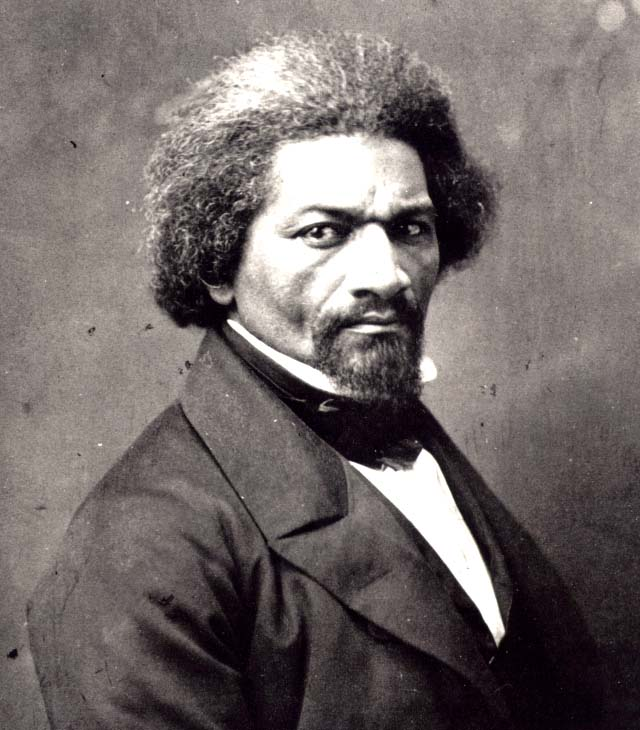
\includegraphics[width=0.6\textwidth]{4fred16b.jpg}\end{figure}
{\em Frederick Douglass, former slave, abolitionist, and engineer on the underground railroad, was a popular speaker on the anti-slavery circuit. He traveled thousands of miles each year, giving hundreds of speeches. Yet the money he earned from lecturing was not enough to become financially comfortable, and he and his family struggled. Douglass was disillusioned by the repercussions of the Fugitive Slave Act, and his abolitionist leanings grew more strident and bold. If the citizens of Rochester, New York had expected to be flattered by Douglass when they asked him to speak on the Fourth, they were soon disavowed of that idea. Douglass took the opportunity to defiantly point out the ripe hypocrisy of a nation celebrating their ideals of freedom and equality while simultaneously mired in the evil of slavery. While the speech surely made even the most liberal audience members squirm; nonetheless, the crowed let loose in “universal applause” when Douglass finished.}

\vspace{10 mm}

Fellow Citizens, I am not wanting in respect for the fathers of this republic. The signers of the Declaration of Independence were brave men. They were great men, too - great enough to give frame to a great age. It does not often happen to a nation to raise, at one time, such a number of truly great men. The point from which I am compelled to view them is not, certainly, the most favorable; and yet I cannot contemplate their great deeds with less than admiration. They were statesmen, patriots and heroes, and for the good they did, and the principles they contended for, I will unite with you to honor their memory….

…Fellow-citizens, pardon me, allow me to ask, why am I called upon to speak here to-day? What have I, or those I represent, to do with your national independence? Are the great principles of political freedom and of natural justice, embodied in that Declaration of Independence, extended to us? and am I, therefore, called upon to bring our humble offering to the national altar, and to confess the benefits and express devout gratitude for the blessings resulting from your independence to us?

Would to God, both for your sakes and ours, that an affirmative answer could be truthfully returned to these questions! Then would my task be light, and my burden easy and delightful. For who is there so cold, that a nation's sympathy could not warm him? Who so obdurate and dead to the claims of gratitude, that would not thankfully acknowledge such priceless benefits? Who so stolid and selfish, that would not give his voice to swell the hallelujahs of a nation's jubilee, when the chains of servitude had been torn from his limbs? I am not that man. In a case like that, the dumb might eloquently speak, and the “lame man leap as an hart.”

But such is not the state of the case. I say it with a sad sense of the disparity between us. I am not included within the pale of glorious anniversary! Your high independence only reveals the immeasurable distance between us. The blessings in which you, this day, rejoice, are not enjoyed in common.‘The rich inheritance of justice, liberty, prosperity and independence, bequeathed by your fathers, is shared by you, not by me. The sunlight that brought light and healing to you, has brought stripes and death to me. This Fourth July is yours, not mine. You may rejoice, I must mourn. To drag a man in fetters into the grand illuminated temple of liberty, and call upon him to join you in joyous anthems, were inhuman mockery and sacrilegious irony. Do you mean, citizens, to mock me, by asking me to speak to-day? If so, there is a parallel to your conduct. And let me warn you that it is dangerous to copy the example of a nation whose crimes, towering up to heaven, were thrown down by the breath of the Almighty, burying that nation in irrevocable ruin! I can to-day take up the plaintive lament of a peeled and woe-smitten people!

“By the rivers of Babylon, there we sat down. Yea! we wept when we remembered Zion. We hanged our harps upon the willows in the midst thereof. For there, they that carried us away captive, required of us a song; and they who wasted us required of us mirth, saying, Sing us one of the songs of Zion. How can we sing the Lord's song in a strange land? If I forget thee, 0 Jerusalem, let my right hand forget her cunning. If I do not remember thee, let my tongue cleave to the roof of my mouth.”

Fellow-citizens, above your national, tumultuous joy, I hear the mournful wail of millions! whose chains, heavy and grievous yesterday, are, to-day, rendered more intolerable by the jubilee shouts that reach them. If I do forget, if I do not faithfully remember those bleeding children of sorrow this day, “may my right hand forget her cunning, and may my tongue cleave to the roof of my mouth!” To forget them, to pass lightly over their wrongs, and to chime in with the popular theme, would be treason most scandalous and shocking, and would make me a reproach before God and the world. My subject, then, fellow-citizens, is American slavery. I shall see this day and its popular characteristics from the slave's point of view. Standing there identified with the American bondman, making his wrongs mine, I do not hesitate to declare, with all my soul, that the character and conduct of this nation never looked blacker to me than on this 4th of July! Whether we turn to the declarations of the past, or to the professions of the present, the conduct of the nation seems equally hideous and revolting. America.is false to the past, false to the present, and solemnly binds herself to be false to the future. Standing with God and the crushed and bleeding slave on this occasion, I will, in the name of humanity which is outraged, in the name of liberty which is fettered, in the name of the constitution and the Bible which are disregarded and trampled upon, dare to call in question and to denounce, with all the emphasis I can command, everything that serves to perpetuate slavery ‘ the great sin and shame of America! “I will not equivocate; I will not excuse”; I will use the severest language I can command; and yet not one word shall escape me that any man, whose judgment is not blinded by prejudice, or who is not at heart a slaveholder, shall not confess to be right and just.

But I fancy I hear some one of my audience say, “It is just in this circumstance that you and your brother abolitionists fail to make a favorable impression on the public mind. Would you argue more, an denounce less; would you persuade more, and rebuke less; your cause would be much more likely to succeed.” But, I submit, where all is plain there is nothing to be argued. What point in the anti-slavery creed would you have me argue? On what branch of the subject do the people of this country need light? Must I undertake to prove that the slave is a man? That point is conceded already. Nobody doubts it. The slaveholders themselves acknowledge it in the enactment of laws for their government. They acknowledge it when they punish disobedience on the part of the slave. There are seventy-two crimes in the State of Virginia which, if committed by a black man (no matter how ignorant he be), subject him to the punishment of death; while only two of the same crimes will subject a white man to the like punishment. What is this but the acknowledgment that the slave is a moral, intellectual, and responsible being? The manhood of the slave is conceded. It is admitted in the fact that Southern statute books are covered with enactments forbidding, under severe fines and penalties, the teaching of the slave to read or to write. When you can point to any such laws in reference to the beasts of the field, then I may consent to argue the manhood of the slave. When the dogs in your streets, when the fowls of the air, when the cattle on your hills, when the fish of the sea, and the reptiles that crawl, shall be unable to distinguish the slave from a brute, then will I argue with you that the slave is a man!

For the present, it is enough to affirm the equal manhood of the Negro race. Is it not astonishing that, while we are ploughing, planting, and reaping, using all kinds of mechanical tools, erecting houses, constructing bridges, building ships, working in metals of brass, iron, copper, silver and gold; that, while we are reading, writing and ciphering, acting as clerks, merchants and secretaries, having among us lawyers, doctors, ministers, poets, authors, editors, orators and teachers; that, while we are engaged in all manner of enterprises common to other men, digging gold in California, capturing the whale in the Pacific, feeding sheep and cattle on the hill-side, living, moving, acting, thinking, planning, living in families as husbands, wives and children, and, above all, confessing and worshipping the Christian's God, and looking hopefully for life and immortality beyond the grave, we are called upon to prove that we are men!

Would you have me argue that man is entitled to liberty? that he is the rightful owner of his own body? You have already declared it. Must I argue the wrongfulness of slavery? Is that a question for Republicans? Is it to be settled by the rules of logic and argumentation, as a matter beset with great difficulty, involving a doubtful application of the principle of justice, hard to be understood? How should I look to-day, in the presence of Amercans, dividing, and subdividing a discourse, to show that men have a natural right to freedom? speaking of it relatively and positively, negatively and affirmatively. To do so, would be to make myself ridiculous, and to offer an insult to your understanding. There is not a man beneath the canopy of heaven that does not know that slavery is wrong for him.

What, am I to argue that it is wrong to make men brutes, to rob them of their liberty, to work them without wages, to keep them ignorant of their relations to their fellow men, to beat them with sticks, to flay their flesh with the lash, to load their limbs with irons, to hunt them with dogs, to sell them at auction, to sunder their families, to knock out their teeth, to burn their flesh, to starve them into obedience and submission to their mastcrs? Must I argue that a system thus marked with blood, and stained with pollution, is wrong? No! I will not. I have better employment for my time and strength than such arguments would imply.

What, then, remains to be argued? Is it that slavery is not divine; that God did not establish it; that our doctors of divinity are mistaken? There is blasphemy in the thought. That which is inhuman, cannot be divine! Who can reason on such a proposition? They that can, may; I cannot. The time for such argument is passed.

At a time like this, scorching irony, not convincing argument, is needed. O! had I the ability, and could reach the nation's ear, I would, to-day, pour out a fiery stream of biting ridicule, blasting reproach, withering sarcasm, and stern rebuke. For it is not light that is needed, but fire; it is not the gentle shower, but thunder. We need the storm, the whirlwind, and the earthquake. The feeling of the nation must be quickened; the conscience of the nation must be roused; the propriety of the nation must be startled; the hypocrisy of the nation must be exposed; and its crimes against God and man must be proclaimed and denounced.

What, to the American slave, is your 4th of July? I answer; a day that reveals to him, more than all other days in the year, the gross injustice and cruelty to which he is the constant victim. To him, your celebration is a sham; your boasted liberty, an unholy license; your national greatness, swelling vanity; your sounds of rejoicing are empty and heartless; your denunciation of tyrants, brass fronted impudence; your shouts of liberty and equality, hollow mockery; your prayers and hymns, your sermons and thanksgivings, with all your religious parade and solemnity, are, to Him, mere bombast, fraud, deception, impiety, and hypocrisy — a thin veil to cover up crimes which would disgrace a nation of savages.There is not a nation on the earth guilty of practices more shocking and bloody than are the people of the United States, at this very hour.

Go where you may, search where you will, roam through all the monarchies and despotisms of the Old World, travel through South America, search out every abuse, and when you have found the last, lay your facts by the side of the everyday practices of this nation, and you will say with me, that, for revolting barbarity and shameless hypocrisy, America reigns without a rival….

…Allow me to say, in conclusion, notwithstanding the dark picture I have this day presented, of the state of the nation, I do not despair of this country. There are forces in operation which must inevitably work the downfall of slavery. “The arm of the Lord is not shortened,” and the doom of slavery is certain. I, therefore, leave off where I began, with hope. While drawing encouragement from “the Declaration of Independence,” the great principles it contains, and the genius of American Institutions, my spirit is also cheered by the obvious tendencies of the age. Nations do not now stand in the same relation to each other that they did ages ago. No nation can now shut itself up from the surrounding world and trot round in the same old path of its fathers without interference. The time was when such could be done. Long established customs of hurtful character could formerly fence themselves in, and do their evil work with social impunity. Knowledge was then confined and enjoyed by the privileged few, and the multitude walked on in mental darkness. But a change has now come over the affairs of mankind. Walled cities and empires have become unfashionable. The arm of commerce has borne away the gates of the strong city. Intelligence is penetrating the darkest corners of the globe. It makes its pathway over and under the sea, as well as on the earth. Wind, steam, and lightning are its chartered agents. Oceans no longer divide, but link nations together. From Boston to London is now a holiday excursion. Space is comparatively annihilated. — Thoughts expressed on one side of the Atlantic are distinctly heard on the other.

The far off and almost fabulous Pacific rolls in grandeur at our feet. The Celestial Empire, the mystery of ages, is being solved. The fiat of the Almighty, “Let there be Light,” has not yet spent its force. No abuse, no outrage whether in taste, sport or avarice, can now hide itself from the all-pervading light. The iron shoe, and crippled foot of China must be seen in contrast with nature. Africa must rise and put on her yet unwoven garment. ‘Ethiopia, shall, stretch. out her hand unto Ood.” In the fervent aspirations of William Lloyd Garrison, I say, and let every heart join in saying it:

\begin{quote}.\end{quote}

\begin{quote}God speed the year of jubilee\end{quote}

\begin{quote}The wide world o'er!\end{quote}

\begin{quote}When from their galling chains set free,\end{quote}

\begin{quote}Th' oppress'd shall vilely bend the knee,\end{quote}

\begin{quote}And wear the yoke of tyranny\end{quote}

\begin{quote}Like brutes no more.\end{quote}

\begin{quote}That year will come, and freedom's reign,\end{quote}

\begin{quote}To man his plundered rights again\end{quote}

\begin{quote}Restore.\end{quote}

\begin{quote}.\end{quote}

\begin{quote}God speed the day when human blood\end{quote}

\begin{quote}Shall cease to flow!\end{quote}

\begin{quote}In every clime be understood,\end{quote}

\begin{quote}The claims of human brotherhood,\end{quote}

\begin{quote}And each return for evil, good,\end{quote}

\begin{quote}Not blow for blow;\end{quote}

\begin{quote}That day will come all feuds to end,\end{quote}

\begin{quote}And change into a faithful friend\end{quote}

\begin{quote}Each foe.\end{quote}

\begin{quote}.\end{quote}

\begin{quote}God speed the hour, the glorious hour,\end{quote}

\begin{quote}When none on earth\end{quote}

\begin{quote}Shall exercise a lordly power,\end{quote}

\begin{quote}Nor in a tyrant's presence cower;\end{quote}

\begin{quote}But to all manhood's stature tower,\end{quote}

\begin{quote}By equal birth!\end{quote}

\begin{quote}That hour will come, to each, to all,\end{quote}

\begin{quote}And from his Prison-house, to thrall\end{quote}

\begin{quote}Go forth.\end{quote}

\begin{quote}.\end{quote}

\begin{quote}Until that year, day, hour, arrive,\end{quote}

\begin{quote}With head, and heart, and hand I'll strive,\end{quote}

\begin{quote}To break the rod, and rend the gyve,\end{quote}

\begin{quote}The spoiler of his prey deprive –\end{quote}

\begin{quote}So witness Heaven!\end{quote}

\begin{quote}And never from my chosen post,\end{quote}

\begin{quote}Whate'er the peril or the cost,\end{quote}

\begin{quote}Be driven.\end{quote}


\chapter{Abraham Lincoln - The Gettysburg Address}

\textbf{\Large{Gettysburg, Pennsylvania -- November 19, 1863 }}

\vspace{10 mm}

\begin{figure}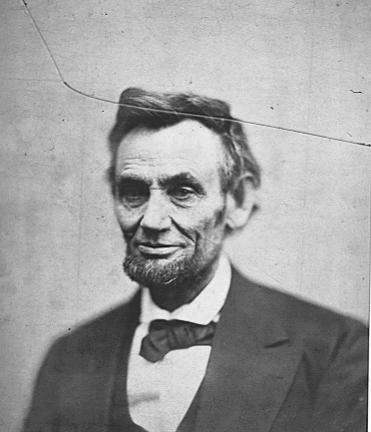
\includegraphics[width=0.6\textwidth]{last_lincoln.jpg}\end{figure}
{\em 272 words. 3 minutes long. Yet, the Gettysburg Address is unarguably one of the greatest pieces of rhetoric in American history. Dr. J Rufus Fears (one of the great modern orators) argues that the Gettysburg Address, along with the Constitution and the Declaration of Independence, form the three founding documents of American freedom. And I have to agree.

The Battle of Gettysburg left 8,000 men dead. The bodies were too numerous to bury properly and many were at first placed in shallow graves. Weeks after the battle, heads and arms were sticking up through the ground and the smell of rotting flesh was sickening.

Money was raised for a proper reburial, and it was decided that the new cemetery should be dedicated, to sweeten the air of Gettysburg, to solemnize this place of death. As was traditional, a great orator, in this case, Edward Everett, was asked to give a solemn and grand speech as a memorial to the fallen men. Lincoln was asked 2 months later, almost as a causal afterthought. He was to add a few remarks to Everett's, a function much like the man with the ceremonial scissors who cuts the ribbon. Legends has it that Lincoln's remarks were the product of pure inspiration, penned on the back of an envelope on the train chugging its way to the soon-to-be hallowed grounds of Gettysburg.

On the day of the dedication, Everett kept the crowd enthralled for a full two hours. Lincoln got up, gave his speech, and sat down even before the photographer had finished setting up for a picture. There was a long pause before anyone applauded, and then the applause was scattered and polite.

Not everyone immediately realized the magnificence of Lincoln's address. But some did. In a letter to Lincoln, Everett praised the President for his eloquent and concise speech, saying, “I should be glad if I could flatter myself that I came as near to the central idea of the occasion, in two hours, as you did in two minutes.”

And of course, in time, we have come to fully appreciate the genius and beauty of the words spoken that day. Dr. Fears argues that Lincoln's address did more than memorialize the fallen soldiers at Gettysburg; it accomplished nothing short of transforming the entire meaning of the Civil War. There were no details of the battle mentioned in the speech, no mentioning of soldier's names, of Gettysburg itself, of the South nor the Union, states rights nor secession. Rather, Lincoln meant the speech to be something far larger, a discourse on the experiment testing whether government can maintain the proposition of equality. At Gettysburg, the Constitution experienced a transformation. The first birth has been tainted by slavery. The men, of both North and South, lying in the graves at Gettysburg had made an atoning sacrifice for this great evil. And the Constitution would be reborn, this time living up to its promises of freedom and equality for all.}

\vspace{10 mm}

Four score and seven years ago our fathers brought forth on this continent, a new nation, conceived in liberty, and dedicated to the proposition that all men are created equal.

Now we are engaged in a great civil war, testing whether that nation, or any nation so conceived and so dedicated, can long endure. We are met on a great battlefield of that war. We have come to dedicate a portion of that field, as a final resting place for those who here gave their lives that that nation might live. It is altogether fitting and proper that we should do this.

But in a larger sense, we cannot dedicate – we cannot consecrate – we cannot hallow – this ground. The brave men, living and dead, who struggled here, have consecrated it, far above our poor power to add or detract. The world will little note, nor long remember, what we say here, but it can never forget what they did here. It is for us the living, rather, to be dedicated here to the unfinished work which they who fought here have thus far so nobly advanced. It is rather for us to be here dedicated to the great task remaining before us – that from these honored dead we take increased devotion to that cause for which they gave the last full measure of devotion – that we here highly resolve that these dead shall not have died in vain – that this nation, under God, shall have a new birth of freedom – and that government of the people, by the people, for the people, shall not perish from the earth.


\chapter{Abraham Lincoln - 2nd Inaugural Address}

\textbf{\Large{Washington D.C. -- March 04, 1865 }}

\vspace{10 mm}

\begin{figure}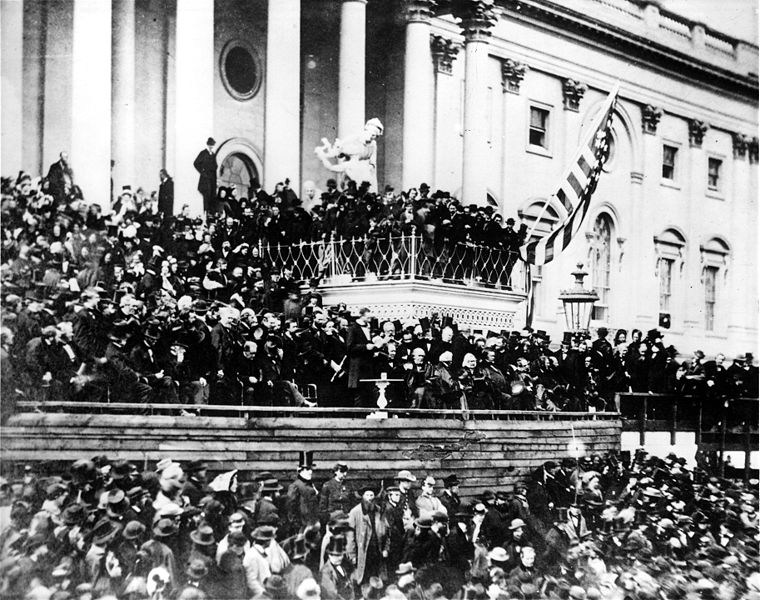
\includegraphics[width=0.6\textwidth]{760px-lincoln_second.jpg}\end{figure}
{\em The Union's victory was but a month away as Abraham Lincoln began his second term as president of a bitterly ruptured United States. Like the Gettysburg Address, Lincoln keeps this speech only as long as needful. While there are those who still debate whether the Civil War was truly fought over slavery or not, Lincoln certainly believed so. To him, slavery was a great national sin, and the blood shed during the war was the atoning sacrifice for that evil.

He does not relish the prospect of coming victory; instead, he appeals to his countrymen to remember that the war was truly fought between brothers. When the war was over and the Confederacy forced to return to the Union, Lincoln was prepared to treat the South with relative leniency. He did not believe secession was truly possible, and thus the South had never truly left the Union. Reconstruction would not mean vengeance, but the return home of a terribly errant son.}

\vspace{10 mm}

Fellow Countrymen:

AT this second appearing to take the oath of the Presidential office there is less occasion for an extended address than there was at the first. Then a statement somewhat in detail of a course to be pursued seemed fitting and proper. Now, at the expiration of four years, during which public declarations have been constantly called forth on every point and phase of the great contest which still absorbs the attention and engrosses the energies of the nation, little that is new could be presented. The progress of our arms, upon which all else chiefly depends, is as well known to the public as to myself, and it is, I trust, reasonably satisfactory and encouraging to all. With high hope for the future, no prediction in regard to it is ventured.

On the occasion corresponding to this four years ago all thoughts were anxiously directed to an impending civil war. All dreaded it, all sought to avert it. While the inaugural address was being delivered from this place, devoted altogether to saving the Union without war, urgent agents were in the city seeking to destroy it without war—seeking to dissolve the Union and divide effects by negotiation. Both parties deprecated war, but one of them would make war rather than let the nation survive, and the other would accept war rather than let it perish, and the war came.

One-eighth of the whole population were colored slaves, not distributed generally over the Union, but localized in the southern part of it. These slaves constituted a peculiar and powerful interest. All knew that this interest was somehow the cause of the war. To strengthen, perpetuate, and extend this interest was the object for which the insurgents would rend the Union even by war, while the Government claimed no right to do more than to restrict the territorial enlargement of it. Neither party expected for the war the magnitude or the duration which it has already attained. Neither anticipated that the cause of the conflict might cease with or even before the conflict itself should cease. Each looked for an easier triumph, and a result less fundamental and astounding. Both read the same Bible and pray to the same God, and each invokes His aid against the other. It may seem strange that any men should dare to ask a just God's assistance in wringing their bread from the sweat of other men's faces, but let us judge not, that we be not judged. The prayers of both could not be answered. That of neither has been answered fully. The Almighty has His own purposes. “Woe unto the world because of offenses; for it must needs be that offenses come, but woe to that man by whom the offense cometh.” If we shall suppose that American slavery is one of those offenses which, in the providence of God, must needs come, but which, having continued through His appointed time, He now wills to remove, and that He gives to both North and South this terrible war as the woe due to those by whom the offense came, shall we discern therein any departure from those divine attributes which the believers in a living God always ascribe to Him? Fondly do we hope, fervently do we pray, that this mighty scourge of war may speedily pass away. Yet, if God wills that it continue until all the wealth piled by the bondsman's two hundred and fifty years of unrequited toil shall be sunk, and until every drop of blood drawn with the lash shall be paid by another drawn with the sword, as was said three thousand years ago, so still it must be said “the judgments of the Lord are true and righteous altogether.”

With malice toward none, with charity for all, with firmness in the right as God gives us to see the right, let us strive on to finish the work we are in, to bind up the nation's wounds, to care for him who shall have borne the battle and for his widow and his orphan, to do all which may achieve and cherish a just and lasting peace among ourselves and with all nations.


\chapter{Chief Joseph - Surrender Speech}

\textbf{\Large{Montana Territory -- October 05, 1877 }}

\vspace{10 mm}

\begin{figure}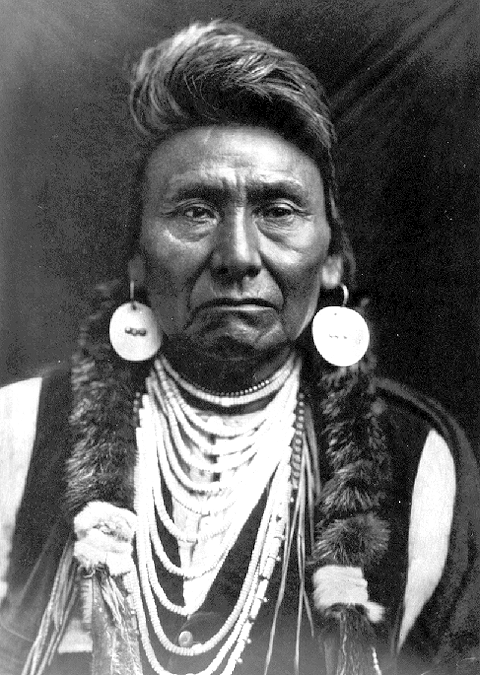
\includegraphics[width=0.6\textwidth]{joold.png}\end{figure}
{\em In 1877, the military announced that the Chief Joseph and his tribe of Nez Perce had to move onto a reservation in Idaho or face retribution. Desiring to avoid violence, Chief Joseph advocated peace and cooperation. But fellow tribesmen dissented and killed four white men. Knowing a swift backlash was coming, Joseph and his people began to make their way to Canada, hoping to find amnesty there. The tribe traveled 1700 miles, fighting the pursuing US army along the way. In dire conditions, and after a five day battle, Chief Joseph surrendered to General Nelson A. Miles on Oct. 5, 1877 in the Bear Paw Mountains of Montana Territory, a mere 40 miles from the Canadian border. The Chief knew he was the last of a dying breed, and the moment of surrender was heartbreaking.}

\vspace{10 mm}

Tell General Howard I know his heart. What he told me before, I have it in my heart. I am tired of fighting. Our Chiefs are killed; Looking Glass is dead, Ta Hool Hool Shute is dead. The old men are all dead. It is the young men who say yes or no. He who led on the young men is dead. It is cold, and we have no blankets; the little children are freezing to death. My people, some of them, have run away to the hills, and have no blankets, no food. No one knows where they are – perhaps freezing to death. I want to have time to look for my children, and see how many of them I can find. Maybe I shall find them among the dead. Hear me, my Chiefs! I am tired; my heart is sick and sad. From where the sun now stands I will fight no more forever.


\chapter{Theodore Roosevelt - Duties of American Citizenship}

\textbf{\Large{Buffalo, New York -- January 26, 1883 }}

\vspace{10 mm}

\begin{figure}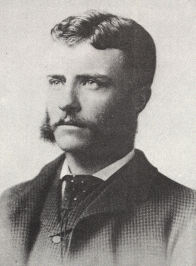
\includegraphics[width=0.6\textwidth]{assemblyman.png}\end{figure}
{\em Given while serving as a New York assemblyman, TR's address on the “Duties of American Citizenship” delved into both the theoretical reasons why every man should be involved in politics and the practical means of serving in that capacity. Roosevelt chided those who excused themselves from politics because they were too busy; it was every man's duty to devote some time to maintaining good government.}

\vspace{10 mm}

Of course, in one sense, the first essential for a man's being a good citizen is his possession of the home virtues of which we think when we call a man by the emphatic adjective of manly. No man can be a good citizen who is not a good husband and a good father, who is not honest in his dealings with other men and women, faithful to his friends and fearless in the presence of his foes, who has not got a sound heart, a sound mind, and a sound body; exactly as no amount of attention to civil duties will save a nation if the domestic life is undermined, or there is lack of the rude military virtues which alone can assure a country's position in the world. In a free republic the ideal citizen must be one willing and able to take arms for the defense of the flag, exactly as the ideal citizen must be the father of many healthy children. A race must be strong and vigorous; it must be a race of good fighters and good breeders, else its wisdom will come to naught and its virtue be ineffective; and no sweetness and delicacy, no love for and appreciation of beauty in art or literature, no capacity for building up material prosperity can possibly atone for the lack of the great virile virtues.

But this is aside from my subject, for what I wish to talk of is the attitude of the American citizen in civic life. It ought to be axiomatic in this country that every man must devote a reasonable share of his time to doing his duty in the Political life of the community. No man has a right to shirk his political duties under whatever plea of pleasure or business; and while such shirking may be pardoned in those of small cleans it is entirely unpardonable in those among whom it is most common–in the people whose circumstances give them freedom in the struggle for life. In so far as the community grows to think rightly, it will likewise grow to regard the young man of means who shirks his duty to the State in time of peace as being only one degree worse than the man who thus shirks it in time of war. A great many of our men in business, or of our young men who are bent on enjoying life (as they have a perfect right to do if only they do not sacrifice other things to enjoyment), rather plume themselves upon being good citizens if they even vote; yet voting is the very least of their duties, Nothing worth gaining is ever gained without effort. You can no more have freedom without striving and suffering for it than you can win success as a banker or a lawyer without labor and effort, without self-denial in youth and the display of a ready and alert intelligence in middle age. The people who say that they have not time to attend to politics are simply saying that they are unfit to live in a free community. Their place is under a despotism; or if they are content to do nothing but vote, you can take despotism tempered by an occasional plebiscite, like that of the second Napoleon. In one of Lowell's magnificent stanzas about the Civil War he speaks of the fact which his countrymen were then learning, that freedom is not a gift that tarries long in the hands of cowards: nor yet does it tarry long in the hands of the sluggard and the idler, in the hands of the man so much absorbed in the pursuit of pleasure or in the pursuit of gain, or so much wrapped up in his own easy home life as to be unable to take his part in the rough struggle with his fellow men for political supremacy. If freedom is worth having, if the right of self-government is a valuable right, then the one and the other must be retained exactly as our forefathers acquired them, by labor, and especially by labor in organization, that is in combination with our fellows who have the same interests and the same principles. We should not accept the excuse of the business man who attributed his failure to the fact that his social duties were so pleasant and engrossing that he had no time left for work in his office; nor would we pay much heed to his further statement that he did not like business anyhow because he thought the morals of the business community by no means what they should be, and saw that the great successes were most often won by men of the Jay Gould stamp. It is just the same way with politics. It makes one feel half angry and half amused, and wholly contemptuous, to find men of high business or social standing in the community saying that they really have not got time to go to ward meetings, to organize political clubs, and to take a personal share in all the important details of practical politics; men who further urge against their going the fact that they think the condition of political morality low, and are afraid that they may be required to do what is not right if they go into politics.

The first duty of an American citizen, then, is that he shall work in politics; his second duty is that he shall do that work in a practical manner; and his third is that it shall be done in accord with the highest principles of honor and justice. Of course, it is not possible to define rigidly just the way in which the work shall be made practical. Each man's individual temper and convictions must be taken into account. To a certain extent his work must be done in accordance with his individual beliefs and theories of right and wrong. To a yet greater extent it must be done in combination with others, he yielding or modifying certain of his own theories and beliefs so as to enable him to stand on a common ground with his fellows, who have likewise yielded or modified certain of their theories and beliefs. There is no need of dogmatizing about independence on the one hand or party allegiance on the other. There are occasions when it may be the highest duty of any man to act outside of parties and against the one with which he has himself been hitherto identified; and there may be many more occasions when his highest duty is to sacrifice some of his own cherished opinions for the sake of the success of the party which he on the whole believes to be right. I do not think that the average citizen, at least in one of our great cities, can very well manage to support his own party all the time on every issue, local and otherwise; at any rate if he can do so he has been more fortunately placed than I have been. On the other hand, I am fully convinced that to do the best work people must be organized; and of course an organization is really a party, whether it be a great organization covering the whole nation and numbering its millions of adherents, or an association of citizens in a particular locality, banded together to win a certain specific victory, as, for instance, that of municipal reform. Somebody has said that a racing-yacht, like a good rifle, is a bundle of incompatibilities; that you must get the utmost possible sail power without sacrificing some other quality if you really do get the utmost sail power, that, in short you have got to make more or less of a compromise on each in order to acquire the dozen things needful; but, of course, in making this compromise you must be very careful for the sake of something unimportant not to sacrifice any of the great principles of successful naval architecture. Well, it is about so with a man's political work. He has got to preserve his independence on the one hand; and on the other, unless he wishes to be a wholly ineffective crank, he has got to have some sense of party allegiance and party responsibility, and he has got to realize that in any given exigency it may be a matter of duty to sacrifice one quality, or it may be a matter of duty to sacrifice the other.

If it is difficult to lay down any fixed rules for party action in the abstract; it would, of course, be wholly impossible to lay them down for party action in the concrete, with reference to the organizations of the present day. I think that we ought to be broad-minded enough to recognize the fact that a good citizen, striving with fearlessness, honesty, and common sense to do his best for the nation, can render service to it in many different ways, and by connection with many different organizations. It is well for a man if he is able conscientiously to feel that his views on the great questions of the day, on such questions as the tariff, finance, immigration, the regulation of the liquor traffic, and others like them, are such as to put him in accord with the bulk of those of his fellow citizens who compose one of the greatest parties: but it is perfectly supposable that he may feel so strongly for or against certain principles held by one party, or certain principles held by the other, that he is unable to give his full adherence to either. In such a case I feel that he has no right to plead this lack of agreement with either party as an excuse for refraining from active political work prior to election. It will, of course, bar him from the primaries of the two leading parties, and preclude him from doing his share in organizing their management; but, unless he is very unfortunate, he can surely find a number of men who are in the same position as himself and who agree with him on some specific piece of political work, and they can turn in practically and effectively long before election to try to do this new piece of work in a practical manner.

One seemingly very necessary caution to utter is, that a man who goes into politics should not expect to reform everything right off, with a jump. I know many excellent young men who, when awakened to the fact that they have neglected their political duties, feel an immediate impulse to form themselves into an organization which shall forthwith purify politics everywhere, national, State, and city alike; and I know of a man who having gone round once to a primary, and having, of course, been unable to accomplish anything in a place where he knew no one and could not combine with anyone, returned saying it was quite useless for a good citizen to try to accomplish anything in such a manner. To these too hopeful or too easily discouraged people I always feel like reading Artemus Ward's article upon the people of his town who came together in a meeting to resolve that the town should support the Union and the Civil War, but were unwilling to take any part in putting down the rebellion unless they could go as brigadier-generals. After the battle of Bull Run there were a good many hundreds of thousands of young men in the North who felt it to be their duty to enter the Northern armies; but no one of them who possessed much intelligence expected to take high place at the outset, or anticipated that individual action would be of decisive importance in any given campaign. He went in as private or sergeant, lieutenant or captain, as the case might be, and did his duty in his company, in his regiment, after a while in his brigade. When Ball's Bluff and Bull Run succeeded the utter failure of the Peninsular campaign, when the terrible defeat of Fredericksburg was followed by the scarcely less disastrous day at Chancellorsville he did not announce (if he had any pluck or manliness about him) that he considered it quite useless for any self-respecting citizen to enter the Army of the Potomac, because he really was not of much weight in its councils, and did not approve of its management; he simply gritted his teeth and went doggedly on with his duty, grieving over, but not disheartened at the innumerable shortcomings and follies committed by those who helped to guide the destinies of the army, recognizing also the bravery, the patience, intelligence, and resolution with which other men in high places offset the follies and shortcomings and persevering with equal mind through triumph and defeat until finally he saw the tide of failure turn at Gettysburg and the full flood of victory come with Appomattox.

I do wish that more of our good citizens would go into politics, and would do it in the same spirit with which their fathers went into the Federal armies. Begin with the little thing, and do not expect to accomplish anything without an effort. Of course, if you go to a primary just once, never having taken the trouble to know any of the other people who go there you will find yourself wholly out of place; but if you keep on attending and try to form associations with other men whom you meet at the political gatherings, or whom you can persuade to attend them, you will very soon find yourself a weight. In the same way, if a man feels that the politics of his city, for instance, are very corrupt and wants to reform them, it would be an excellent idea for him to begin with his district. If he Joins with other people, who think as he does, to form a club where abstract political virtue will be discussed he may do a great deal of good. We need such clubs; but he must also get to know his own ward or his own district, put himself in communication with the decent people in that district, of whom we may rest assured there will be many, willing and able to do something practical for the procurance of better government Let him set to work to procure a better assemblyman or better alderman before he tries his hand at making a mayor, a governor, or a president. If he begins at the top he may make a brilliant temporary success, but the chances are a thousand to one that he will only be defeated eventually; and in no event will the good he does stand on the same broad and permanent foundation as if he had begun at the bottom. Of course, one or two of his efforts may be failures; but if he has the right stuff in him he will go ahead and do his duty irrespective of whether he meets with success or defeat. It is perfectly right to consider the question of failure while shaping one's efforts to succeed in the struggle for the right; but there should be no consideration of it whatsoever when the question is as to whether one should or should not make a struggle for the right. When once a band of one hundred and fifty or two hundred honest, intelligent men, who mean business and know their business, is found in any district, whether in one of the regular organizations or outside, you can guarantee that the local politicians of that district will begin to treat it with a combination of fear, hatred, and respect, and that its influence will be felt; and that while sometimes men will be elected to office in direct defiance of its wishes, more often the successful candidates will feel that they have to pay some regard to its demands for public decency and honesty.

But in advising you to be practical and to work hard, I must not for one moment be understood as advising you to abandon one iota of your self-respect and devotion to principle. It is a bad sign for the country to see one class of our citizens sneer at practical politicians, and another at Sunday-school politics. No man can do both effective and decent work in public life unless he is a practical politician on the one hand, and a sturdy believer in Sunday-school politics on the other. He must always strive manfully for the best, and yet, like Abraham Lincoln, must often resign himself to accept the best possible. Of course when a man verges on to the higher ground of statesmanship, when he becomes a leader, he must very often consult with others and defer to their opinion, and must be continually settling in his mind how far he can go in just deference to the wishes and prejudices of others while yet adhering to his own moral standards: but I speak not so much of men of this stamp as I do of the ordinary citizen, who wants to do his duty as a member of the commonwealth in its civic life; and for this man I feel that the one quality which he ought always to hold most essential is that of disinterestedness. If he once begins to feel that he wants office himself, with a willingness to get it at the cost of his convictions, or to keep it when gotten, at the cost of his convictions, his usefulness is gone. Let him make up his mind to do his duty in politics without regard to holding office at all, and let him know that often the men in this country who have done the best work for our public life have not been the men in office. If, on the other hand, he attains public position, let him not strive to plan out for himself a career. I do not think that any man should let himself regard his political career as a means of livelihood, or as his sole occupation in life; for if he does he immediately becomes most seriously handicapped. The moment that he begins to think how such and such an act will affect the voters in his district, or will affect some great political leader who will have an influence over his destiny, he is hampered and his hands are bound. Not only may it be his duty often to disregard the wishes of politicians, but it may be his clear duty at times to disregard the wishes of the people. The voice of the people is not always the voice of God; and when it happens to be the voice of the devil, then it is a man's clear duty to defy its behests. Different political conditions breed different dangers. The demagogue is as unlovely a creature as the courtier, though one is fostered under republican and the other under monarchical institutions. There is every reason why a man should have an honorable ambition to enter public life, and an honorable ambition to stay there when he is in; but he ought to make up his mind that he cares for it only as long as he can stay in it on his own terms, without sacrifice of his own principles; and if he does thus make up his mind he can really accomplish twice as much for the nation, and can reflect a hundredfold greater honor upon himself, in a short term of service, than can the man who grows gray in the public employment at the cost of sacrificing what he believes to be true and honest. And moreover, when a public servant has definitely made up his mind that he will pay no heed to his own future, but will do what he honestly deems best for the community, without regard to how his actions may affect his prospects, not only does he become infinitely more useful as a public servant, but he has a far better time. He is freed from the harassing care which is inevitably the portion of him who is trying to shape his sails to catch every gust of the wind of political favor.

But let me reiterate, that in being virtuous he must not become ineffective, and that he must not excuse himself for shirking his duties by any false plea that he cannot do his duties and retain his self-respect. This is nonsense, he can; and when he urges such a plea it is a mark of mere laziness and self-indulgence. And again, he should beware how he becomes a critic of the actions of others, rather than a doer of deeds himself; and in so far as he does act as a critic (and of course the critic has a great and necessary function) he must beware of indiscriminate censure even more than of indiscriminate praise. The screaming vulgarity of the foolish spread-eagle orator who is continually yelling defiance at Europe, praising everything American, good and bad, and resenting the introduction of any reform because it has previously been tried successfully abroad, is offensive and contemptible to the last degree; but after all it is scarcely as harmful as the peevish, fretful, sneering, and continual faultfinding of the refined, well-educated man, who is always attacking good and bad alike, who genuinely distrusts America, and in the true spirit of servile colonialism considers us inferior to the people across the water. It may be taken for granted that the man who is always sneering at our public life and our public men is a thoroughly bad citizen, and that what little influence he wields in the community is wielded for evil. The public speaker or the editorial writer who teaches men of education that their proper attitude toward American politics should be one of dislike or indifference is doing all he can to perpetuate and aggravate the very evils of which he is ostensibly complaining. Exactly as it is generally the case that when a man bewails the decadence of our civilization he is himself physically, mentally, and morally a first-class type of the decadent, so it is usually the case that when a man is perpetually sneering at American politicians, whether worthy or unworthy, he himself is a poor citizen and a friend of the very forces of evil against which he professes to contend. Too often these men seem to care less for attacking bad men, than for ruining the characters of good men with whom they disagree on some pubic question; and while their influence against the bad is almost nil, they are sometimes able to weaken the hands of the good by withdrawing from them support to which they are entitled, and they thus count in the sum total of forces that work for evil. They answer to the political prohibitionist, who, in a close contest between a temperance man and a liquor seller diverts enough votes from the former to elect the liquor seller Occasionally it is necessary to beat a pretty good man, who is not quite good enough, even at the cost of electing a bad one- but it should be thoroughly recognized that this can be necessary only occasionally and indeed, I may say, only in very exceptional cases, and that as a rule where it is done the effect is thoroughly unwholesome in every way, and those taking part in it deserve the severest censure from all honest men.

Moreover, the very need of denouncing evil makes it all the more wicked to weaken the effect of such denunciations by denouncing also the good. It is the duty of all citizens, irrespective of party, to denounce, and, so far as may be, to punish crimes against the public on the part of politicians or officials. But exactly as the public man who commits a crime against the public is one of the worst of criminals, so, close on his heels in the race for iniquitous distinction, comes the man who falsely charges the public servant with outrageous wrongdoing; whether it is done with foul-mouthed and foolish directness in the vulgar and violent party organ, or with sarcasm, innuendo, and the half-truths that are worse than lies, in some professed organ of independence. Not only should criticism be honest, but it should be intelligent, in order to be effective. I recently read in a religious paper an article railing at the corruption of our public life, in which it stated incidentally that the lobby was recognized as all-powerful in Washington. This is untrue. There was a day when the lobby was very important at Washington, but its influence in Congress is now very small indeed; and from a pretty intimate acquaintance with several Congresses I am entirely satisfied that there is among the members a very small proportion indeed who are corruptible, in the sense that they will let their action be influenced by money or its equivalent. Congressmen are very often demagogues; they are very often blind partisans; they are often exceedingly short-sighted, narrow-minded, and bigoted; but they are not usually corrupt; and to accuse a narrow-minded demagogue of corruption when he is perfectly honest, is merely to set him more firmly in his evil course and to help him with his constituents, who recognize that the charge is entirely unjust, and in repelling it lose sight of the man's real shortcomings. I have known more than one State legislature, more than one board of aldermen against which the charge of corruption could perfectly legitimately be brought, but it cannot be brought against Congress. Moreover these sweeping charges really do very little good. When I was in the New York legislature, one of the things that I used to mind most was the fact that at the close of every session the papers that affect morality invariably said that particular legislature was the worst legislature since the days of Tweed. The statement was not true as a rule; and, in any event, to lump all the members, good and bad, in sweeping condemnation simply hurt the good and helped the bad. Criticism should be fearless, but I again reiterate that it should be honest and should be discriminating. When it is sweeping and unintelligent, and directed against good and bad alike, or against the good and bad qualities of any man alike, it is very harmful. It tends steadily to deteriorate the character of our public men; and it tends to produce a very unwholesome spirit among young men of education, and especially among the young men in our colleges.

Against nothing is fearless and specific criticism more urgently needed than against the “spoils system,” which is the degradation of American politics. And nothing is more effective in thwarting the purposes of the spoilsmen than the civil service reform. To be sure, practical politicians sneer at it. One of them even went so far as to say that civil-service reform is asking a man irrelevant questions. What more irrelevant question could there be than that of the practical politician who asks the aspirant for his political favor – “Whom did you vote for in the last election?” There is certainly nothing more interesting, from a humorous point of view, than the heads of departments urging changes to be made in their underlings, “on the score of increased efficiency” they say; when as the result of such a change the old incumbent often spends six months teaching the new incumbent how to do the work almost as well as he did himself! Occasionally the civil-service reform has been abused, but not often. Certainly the reform is needed when you contemplate the spectacle of a New York City treasurer who acknowledges his annual fees to be eighty-five thousand dollars, and who pays a deputy one thousand five hundred dollars to do his work-when you note the corruptions in the New York legislature, where one man says he has a horror of the Constitution because it prevents active benevolence, and another says that you should never allow the Constitution to come between friends! All these corruptions and vices are what every good American citizen must fight against.

Finally, the man who wishes to do his duty as a citizen in our country must be imbued through and through with the spirit of Americanism. I am not saying this as a matter of spread-eagle rhetoric: I am saying it quite soberly as a piece of matter-of-fact, common-sense advice, derived from my own experience of others. Of course, the question of Americanism has several sides. If a man is an educated man, he must show his Americanism by not getting misled into following out and trying to apply all the theories of the political thinkers of other countries, such as Germany and France, to our own entirely different conditions. He must not get a fad, for instance, about responsible government; and above all things he must not, merely because he is intelligent, or a college professor well read in political literature, try to discuss our institutions when he has had no practical knowledge of how they are worked. Again, if he is a wealthy man, a man of means and standing, he must really feel, not merely affect to feel, that no social differences obtain save such as a man can in some way himself make by his own actions. People sometimes ask me if there is not a prejudice against a man of wealth and education in ward politics. I do not think that there is, unless the man in turn shows that he regards the facts of his having wealth and education as giving him a claim to superiority aside from the merit he is able to prove himself to have in actual service. Of course, if he feels that he ought to have a little better treatment than a carpenter, a plumber, or a butcher, who happens to stand beside him, he is going to be thrown out of the race very quickly, and probably quite roughly; and if he starts in to patronize and elaborately condescend to these men he will find that they resent this attitude even more. Do not let him think about the matter at all. Let him go into the political contest with no more thought of such matters than a college boy gives to the social standing of the members of his own and rival teams in a hotly contested football match. As soon as he begins to take an interest in politics (and he will speedily not only get interested for the sake of politics, but also take a good healthy interest in playing the game itself – an interest which is perfectly normal and praise-worthy, and to which only a prig would object), he will begin to work up the organization in the way that will be most effective, and he won't care a rap about who is put to work with him, save in so far as he is a good fellow and an efficient worker. There was one time that a number of men who think as we do here to-night (one of the number being myself) got hold of one of the assembly districts of New York, and ran it in really an ideal way, better than any other assembly district has ever been run before or since by either party. We did it by hard work and good organization; by working practically, and yet by being honest and square in motive and method: especially did we do it by all turning in as straight-out Americans without any regard to distinctions of race origin. Among the many men who did a great deal in organizing our victories was the son of a Presbyterian clergyman, the nephew of a Hebrew rabbi, and two well-known Catholic gentlemen. We also had a Columbia College professor (the stroke-oar of a university crew), a noted retail butcher, and the editor of a local German paper, various brokers, bankers, lawyers, bricklayers and a stone-mason who was particularly useful to us, although on questions of theoretic rather than applied politics he had a decidedly socialistic turn of mind.

Again, questions of race origin, like questions of creed, must not be considered: we wish to do good work, and we are all Americans, pure and simple. In the New York legislature, when it fell to my lot to choose a committee – which I always esteemed my most important duty at Albany – no less than three out of the four men I chose were of Irish birth or parentage; and three abler and more fearless and disinterested men never sat in a legislative body; while among my especial political and personal friends in that body was a gentleman from the southern tier of counties, who was, I incidentally found out, a German by birth, but who was just as straight United States as if his ancestors had come over here in the Mayflower or in Henry Hudson's yacht. Of course, none of these men of Irish or German birth would have been worth their salt had they continued to act after coming here as Irishmen or Germans, or as anything but plain straight-out Americans. We have not any room here for a divided allegiance. A man has got to be an American and nothing else; and he has no business to be mixing us up with questions of foreign politics, British or Irish, German or French, and no business to try to perpetuate their language and customs in the land of complete religious toleration and equality. If, however, he does become honestly and in good faith an American, then he is entitled to stand precisely as all other Americans stand, and it is the height of un-Americanism to discriminate against him in any way because of creed or birthplace. No spirit can be more thoroughly alien to American institutions, than the spirit of the Know-Nothings.

In facing the future and in striving, each according to the measure of his individual capacity, to work out the salvation of our land, we should be neither timid pessimists nor foolish optimists. We should recognize the dangers that exist and that threaten us: we should neither overestimate them nor shrink from them, but steadily fronting them should set to work to overcome and beat them down. Grave perils are yet to be encountered in the stormy course of the Republic – perils from political corruption, perils from individual laziness, indolence and timidity, perils springing from the greed of the unscrupulous rich, and from the anarchic violence of the thriftless and turbulent poor. There is every reason why we should recognize them, but there is no reason why we should fear them or doubt our capacity to overcome them, if only each will, according to the measure of his ability, do his full duty, and endeavor so to live as to deserve the high praise of being called a good American citizen.


\chapter{Theodore Roosevelt - Strength and Decency}

\textbf{\Large{Washington D.C. -- August 16, 1903 }}

\vspace{10 mm}

\begin{figure}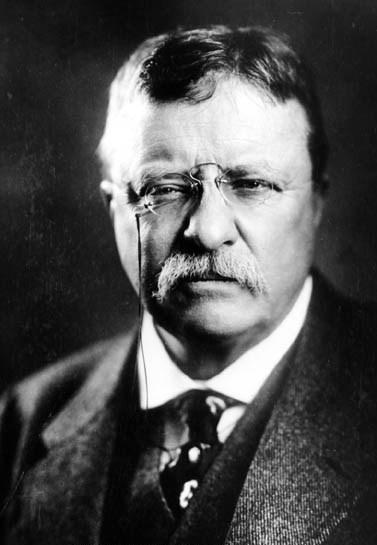
\includegraphics[width=0.6\textwidth]{teddy_close.jpg}\end{figure}
{\em Roosevelt was an advocate of having many children and making sure the next generation would continue to uphold the great virtues of civilization. He was always concerned that young men not be coddled or cowardly, and grow up to live rugged, strenuous, and thoroughly manly lives. But he also strongly believed that being ruggedly manly and being refined in mind and spirit were not incompatible and should in fact go hand and hand. In this speech, he exhorts young men to pursue virtuous manliness. Amen, brother, amen.}

\vspace{10 mm}

I AM particularly glad to see such a society as this flourishing as your society has flourished, because the future welfare of our nation depends upon the way in which we can combine in our men – in our young men – decency and strength. Just this morning when attending service on the great battleship Kearsarge I listened to a sermon addressed to the officers and enlisted men of the navy, in which the central thought was that each American must be a good man or he could not be a good citizen. And one of the things dwelt upon in that sermon was the fact that a man must be clean of mouth as well as clean of life – must show by his words as well as by his actions his fealty to the Almighty if he was to be what we have a right to expect from men wearing the national uniform. We have good Scriptural authority for the statement that it is not what comes into a man's mouth but what goes out of it that counts. I am not addressing weaklings, or I should not take the trouble to come here. I am addressing strong, vigorous men, who are engaged in the active hard work of life; and life to be worth living must be a life of activity and hard work. I am speaking to men engaged in the hard, active work of life, and therefore to men who will count for good or for evil.

It is peculiarly incumbent upon you who have strength to set a right example to others. I ask you to remember that you cannot retain your self-respect if you are loose and foul of tongue, that a man who is to lead a clean and honorable life must inevitably suffer if his speech likewise is not clean and honorable. Every man here knows the temptations that beset all of us in this world. At times any man will slip. I do not expect perfection, but I do expect genuine and sincere effort toward being decent and cleanly in thought, in word, and in deed. As I said at the outset, I hail the work of this society as typifying one of those forces which tend to the betterment and uplifting of our social system. Our whole effort should be toward securing a combination of the strong qualities with those qualities which we term virtues. I expect you to be strong. I would not respect you if you were not. I do not want to see Christianity professed only by weaklings; I want to see it a moving spirit among men of strength. I do not expect you to lose one particle of your strength or courage by being decent. On the contrary, I should hope to see each man who is a member of this society, from his membership in it become all the fitter to do the rough work of the world; all the fitter to work in time of peace; and if, which may Heaven forfend, war should come, all the fitter to fight in time of war. I desire to see in this country the decent men strong and the strong men decent, and until we get that combination in pretty good shape we are not going to be by any means as successful as we should be. There is always a tendency among very young men and among boys who are not quite young men as yet to think that to be wicked is rather smart; to think it shows that they are men. Oh, how often you see some young fellow who boasts that he is going to “see life,” meaning by that that he is going to see that part of life which it is a thousandfold better should remain unseen! I ask that every man here constitute himself his brother's keeper by setting an example to that younger brother which will prevent him from getting such a false estimate of life. Example is the most potent of all things. If any one of you in the presence of younger boys, and especially the younger people of our own family, misbehave yourself, if you use coarse and blasphemous language before them, you can be sure that these younger people will follow your example and not your precept. It is no use to preach to them if you do not act decently yourself. You must feel that the most effective way in which you can preach is by your practice.

As I was driving up here a friend who was with us said that in his experience the boy who went out into life with a foul tongue was apt so to go because his kinsfolk, at least his intimate associates, themselves had foul tongues. The father, the elder brothers, the friends, can do much toward seeing that the boys as they become men become clean and honorable men.

I have told you that I wanted you not only to be decent, but to be strong. These boys will not admire virtue of a merely anaemic type. They believe in courage, in manliness. They admire those who have the quality of being brave, the quality of facing life as life should be faced, the quality that must stand at the root of good citizenship in peace or in war. If you are to be effective as good Christians you must possess strength and courage, or your example will count for little with the young, who admire strength and courage. I want to see you, the men of the Holy Name Society, you who embody the qualities which the younger people admire, by your example give those young people the tendency, the trend, in the right direction; and remember that this example counts in many other ways besides cleanliness of speech. I want to see every man able to hold his own with the strong, and also ashamed to oppress the weak. I want to see each young fellow able to do a man's work in the world, and of a type which will not permit imposition to be practised upon him. I want to see him too strong of spirit to submit to wrong, and, on the other hand, ashamed to do wrong to others. I want to see each man able to hold his own in the rough work of actual life outside, and also, when he is at home, a good man, unselfish in dealing with wife, or mother, or children. Remember that the preaching does not count if it is not backed up by practice. There is no good in your preaching to your boys to be brave if you run away. There is no good in your preaching to them to tell the truth if you do not. There is no good in your preaching to them to be unselfish if they see you selfish with your wife, disregardful of others. We have a right to expect that you will come together in meetings like this; that you will march in processions; that you will join in building up such a great and useful association as this; and, even more, we have a right to expect that in your own homes and among your own associates you will prove by your deeds that yours is not a lip-loyalty merely; that you show in actual practice the faith that is in you.


\chapter{Theodore Roosevelt - The Main with the Muck-rake}

\textbf{\Large{Washington D.C. -- April 14, 1906 }}

\vspace{10 mm}

\begin{figure}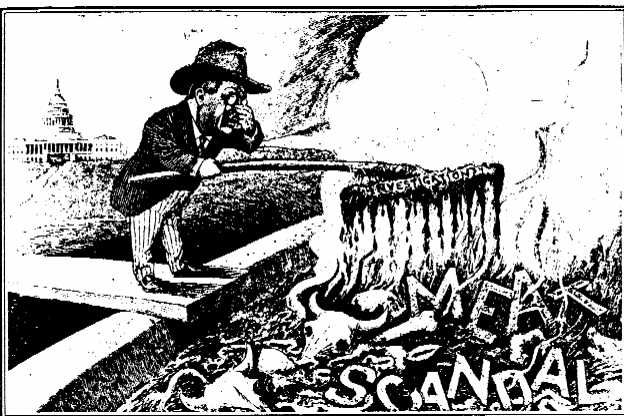
\includegraphics[width=0.6\textwidth]{trtoonmuck.jpg}\end{figure}
{\em Theodore Roosevelt was president during the Progressive Era, a time of great enthusiasm for reform in government, the economy, and society. TR himself held many progressive ideals, but he also called for moderation, not extremism. The “Man with a Muck-rake” in Pilgrim's Progress never looked heavenward but instead constantly raked the filth at his feet. TR thus dubbed the journalists and activists of the day who were intent on exposing the corruption in society as “muckrakers.” He felt that they did a tremendous amount of good, but needed to mitigate their constant pessimism and alarmist tone. He worried that the sensationalism with which these exposes were often presented would make citizens overly cynical and too prone to throw out the baby with the bathwater.}

\vspace{10 mm}

Over a century ago Washington laid the corner-stone of the Capitol in what was then little more than a tract of wooded wilderness here beside the Potomac. We now find it necessary to provide great additional buildings for the business of the government. This growth in the need for the housing of the government is but a proof and example of the way in which the nation has grown and the sphere of action of the National Government has grown. We now administer the affairs of a nation in which the extraordinary growth of population has been outstripped by the growth of wealth and the growth in complex interests.

The material problems that face us to-day are not such as they were in Washington's time, but the underlying facts of human nature are the same now as they were then. Under altered external form we war with the same tendencies toward evil that were evident in Washington's time, and are helped by the same tendencies for good.

It is about some of these that I wish to say a word to-day. In Bunyan's “Pilgrim's Progress” you may recall the description of the Man with the Muck-rake, the man who could look no way but downward, with the muck-rake in his hand; who was offered a celestial crown for his muck-rake, but who would neither look up nor regard the crown he was offered, but continued to rake to himself the filth of the floor.

In “Pilgrim's Progress” the Man with the Muck-rake is set forth as the example of him whose vision is fixed on carnal instead of on spiritual things. Yet he also typifies the man who in this life consistently refuses to see aught that is lofty, and fixes his eyes with solemn intentness only on that which is vile and debasing. Now, it is very necessary that we should not flinch from seeing what is vile and debasing. There is filth on the floor and it must be scraped up with the muck-rake; and there are times and places where this service is the most needed of all the services that can be performed. But the man who never does anything else, who never thinks or speaks or writes, save of his feats with the muck-rake, speedily becomes, not a help to society, not an incitement to good, but one of the most potent forces for evil.

There are, in the body politic, economic and social, many and grave evils, and there is urgent necessity for the sternest war upon them. There should be relentless exposure of and attack upon every evil man whether politician or business man, every evil practice, whether in politics, in business, or in social life. I hail as a benefactor every writer or speaker, every man who, on the platform, or in book, magazine, or newspaper, with merciless severity makes such attack, provided always that he in his turn remembers that the attack is of use only if it is absolutely truthful. The liar is no whit better than the thief, and if his mendacity takes the form of slander, he may be worse than most thieves. It puts a premium upon knavery untruthfully to attack an honest man, or even with hysterical exaggeration to assail a bad man with untruth. An epidemic of indiscriminate assault upon character does not good, but very great harm. The soul of every scoundrel is gladdened whenever an honest man is assailed, or even when a scoundrel is untruthfully assailed.

Now, it is easy to twist out of shape what I have just said, easy to affect to misunderstand it, and, if it is slurred over in repetition, not difficult really to misunderstand it. Some persons are sincerely incapable of understanding that to denounce mud-slinging does not mean the endorsement of whitewashing; and both the interested individuals who need whitewashing, and those others who practice mud-slinging, like to encourage such confusion of ideas. One of the chief counts against those who make indiscriminate assault upon men in business or men in public life, is that they invite a reaction which is sure to tell powerfully in favor of the unscrupulous scoundrel who really ought to be attacked, who ought to be exposed, who ought, if possible, to be put in the penitentiary. If Aristides is praised overmuch as just, people get tired of hearing it; and overcensure of the unjust finally and from similar reasons results in their favor.

Any excess is almost sure to invite a reaction; and, unfortunately, the reaction, instead of taking the form of punishment of those guilty of the excess, is very apt to take the form either of punishment of the unoffending or of giving immunity, and even strength, to offenders. The effort to make financial or political profit out of the destruction of character can only result in public calamity. Gross and reckless assaults on character, whether on the stump or in newspaper, magazine, or book, create a morbid and vicious public sentiment, and at the same time act as a profound deterrent to able men of normal sensitiveness and tend to prevent them from entering the public service at any price.

As an instance in point, I may mention that one serious difficulty encountered in getting the right type of men to dig the Panama Canal is the certainty that they will be exposed, both without, and, I am sorry to say, sometimes within, Congress, to utterly reckless assaults on their character and capacity.

At the risk of repetition let me say again that my plea is, not for immunity to but for the most unsparing exposure of the politician who betrays his trust, of the big business man who makes or spends his fortune in illegitimate or corrupt ways. There should be a resolute effort to hunt every such man out of the position he has disgraced. Expose the crime, and hunt down the criminal; but remember that even in the case of crime, if it is attacked in sensational, lurid, and untruthful fashion, the attack may do more damage to the public mind than the crime itself. It is because I feel that there should be no rest in the endless war against the forces of evil that I ask that the war be conducted with sanity as well as with resolution.

The men with the muck-rakes are often indispensable to the well-being of society; but only if they know when to stop raking the muck, and to look upward to the celestial crown above them, to the crown of worthy endeavor.

There are beautiful things above and roundabout them; and if they gradually grow to feel that the whole world is nothing but muck, their power of usefulness is gone. If the whole picture is painted black there remains no hue whereby to single out the rascals for distinction from their fellows. Such painting finally induces a kind of moral color-blindness; and people affected by it come to the conclusion that no man is really black, and no man is really white, but they are all gray. In other words, they neither believe in the truth of the attack, nor in the honesty of the man who is attacked; they grow as suspicious of the accusation as of the offense; it becomes well-nigh hopeless to stir them either to wrath against wrong-doing or to enthusiasm for what is right; and such a mental attitude in the public gives hope to every knave, and is the despair of honest men.

To assail the great and admitted evils of our political and industrial life with such crude and sweeping generalizations as to include decent men in the general condemnation means the searing of the public conscience. There results a general attitude either of cynical belief in and indifference to public corruption or else of a distrustful inability to discriminate between the good and the bad. Either attitude is fraught with untold damage to the country as a whole. The fool who has not sense to discriminate between what is good and what is bad is well-nigh as dangerous as the man who does discriminate and yet chooses the bad. There is nothing more distressing to every good patriot, to every good American, than the hard, scoffing spirit which treats the allegation of dishonesty in a public man as a cause for laughter.

Such laughter is worse than the crackling of thorns under a pot, for it denotes not merely the vacant mind, but the heart in which high emotions have been choked before they could grow to fruition.

There is any amount of good in the world, and there never was a time when loftier and more disinterested work for the betterment of mankind was being done than now. The forces that tend for evil are great and terrible, but the forces of truth and love and courage and honesty and generosity and sympathy are also stronger than ever before. It is a foolish and timid, no less than a wicked, thing to blink the fact that the forces of evil are strong, but it is even worse to fail to take into account the strength of the forces that tell for good.

Hysterical sensationalism is the very poorest weapon wherewith to fight for lasting righteousness. The men who with stern sobriety and truth assail the many evils of our time, whether in the public press or in magazines, or in books, are the leaders and allies of all engaged in the work for social and political betterment. But if they give good reason for distrust of what they say, if they chill the ardor of those who demand truth as a primary virtue, they thereby betray the good cause, and play into the hands of the very men against whom they are nominally at war.

In his “Ecclesiastical Polity” that fine old Elizabethan divine, Bishop Hooker, wrote: “He that goeth about to persuade a multitude that they are not so well governed as they ought to be, shall never want attentive and favorable hearers; because they know the manifold defects whereunto every kind of regimen is subject, but the secret lets and difficulties, which in public proceedings are innumerable and inevitable, they have not ordinarily the judgment to consider.”

This truth should be kept constantly in mind by every free people desiring to preserve the sanity and poise indispensable to the permanent success of self-government. Yet, on the other hand, it is vital not to permit this spirit to sanity and self-command to degenerate into mere mental stagnation. Bad though a state of hysterical excitement is, and evil though the results are which come from the violent oscillations such excitement invariably produces, yet a sodden acquiescence in evil is even worse.

At this moment we are passing through a period of great unrest-social, political, and industrial unrest. It is of the utmost importance for our future that this should prove to be not the unrest of mere rebelliousness against life, of mere dissatisfaction with the inevitable inequality of conditions, but the unrest of a resolute and eager ambition to secure the betterment of the individual and the nation. So far as this movement of agitation throughout the country takes the form of a fierce discontent with evil, of a determination to punish the authors of evil, whether in industry or politics, the feeling is to be heartily welcomed as a sign of healthy life.

If, on the other hand, it turns into a mere crusade of appetite against appetite, of a contest between the brutal greed of the “have-nots” and the brutal greed of the “haves,” then it has no significance for good, but only for evil. If it seeks to establish a line of cleavage, not along the line which divides good men from bad, but along that other line, running at right angles thereto, which divides those who are well off from those who are less well off, then it will be fraught with immeasurable harm to the body politic.

We can no more and no less afford to condone evil in the man of capital than evil in the man of no capital. The wealthy man who exults because there is a failure of justice in the effort to bring some trust magnate to an account for his misdeeds is as bad as, and no worse than, the so-called labor leader who clamorously strives to excite a foul class feeling on behalf of some other labor leader who is implicated in murder. One attitude is as bad as the other, and no worse; in each case the accused is entitled to exact justice; and in neither case is there need of action by others which can be construed into an expression of sympathy for crime.

It is a prime necessity that if the present unrest is to result in permanent good the emotion shall be translated into action, and that the action shall be marked by honesty, sanity, and self-restraint. There is mighty little good in a mere spasm of reform. The reform that counts is that which comes through steady, continuous growth; violent emotionalism leads to exhaustion.

It is important to this people to grapple with the problems connected with the amassing of enormous fortunes, and the use of those fortunes, both corporate and individual, in business. We should discriminate in the sharpest way between fortunes well-won and fortunes ill-won; between those gained as an incident to performing great services to the community as a whole, and those gained in evil fashion by keeping just within the limits of mere law-honesty.

Of course no amount of charity in spending such fortunes in any way compensates for misconduct in making them. As a matter of personal conviction, and without pretending to discuss the details or formulate the system, I feel that we shall ultimately have to consider the adoption of some such scheme as that of a progressive tax on all fortunes, beyond a certain amount either given in life or devised or bequeathed upon death to any individual-a tax so framed as to put it out of the power of the owner of one of these enormous fortunes to hand on more than a certain amount to any one individual; the tax, of course, to be imposed by the National and not the State Government.

Such taxation should, of course, be aimed merely at the inheritance or transmission in their entirety of those fortunes swollen beyond all healthy limits. Again, the National Government must in some form exercise supervision over corporations engaged in interstate business-and all large corporations are engaged in interstate business-whether by license or otherwise, so as to permit us to deal with the far-reaching evils of overcapitalization.

This year we are making a beginning in the direction of serious effort to settle some of these economic problems by the railway-rate legislation. Such legislation, if so framed, as I am sure it will be, as to secure definite and tangible results, will amount to something of itself; and it will amount to a great deal more in so far as it is taken as a first step in the direction of a policy of superintendence and control over corporate wealth engaged in interstate commerce, this superintendence and control not to be exercised in a spirit of malevolence toward the men who have created the wealth, but with the firm purpose both to do justice to them and to see that they in their turn do justice to the public at large.

The first requisite in the public servants who are to deal in this shape with corporations, whether as legislators or as executives, is honesty. This honesty can be no respecter of persons. There can be no such thing as unilateral honesty. The danger is not really from corrupt corporations; it springs from the corruption itself, whether exercised for or against corporations.

The eighth commandment reads: “Thou shalt not steal.” It does not read: “Thou shalt not steal from the rich man.” It does not read: “Thou shalt not steal from the poor man.” It reads simply and plainly: “Thou shalt not steal.”

No good whatever will come from that warped and mock morality which denounces the misdeeds of men of wealth and forgets the misdeeds practiced at their expense; which denounces bribery, but blinds itself to blackmail; which foams with rage if a corporation secures favors by improper methods, and merely leers with hideous mirth if the corporation is itself wronged. The only public servant who can be trusted honestly to protect the rights of the public against the misdeeds of a corporation is that public man who will just as surely protect the corporation itself from wrongful aggression.

If a public man is willing to yield to popular clamor and do wrong to the men of wealth or to rich corporations, it may be set down as certain that if the opportunity comes he will secretly and furtively do wrong to the public in the interest of a corporation.

But, in addition to honesty, we need sanity. No honesty will make public man useful if that man is timid or foolish, if he is a hot-headed zealot or an impracticable visionary.

As we strive for reform we find that it is not at all merely the case of a long up-hill pull. On the contrary, there is almost as much of breeching work as of collar work; to depend only on traces means that there will soon be a runaway and an upset.

The men of wealth who today are trying to prevent the regulation and control of their business in the interest of the public by the proper government authorities will not succeed, in my judgment, in checking the progress of the movement. But if they did succeed they would find that they had sown the wind and would surely reap the whirlwind, for they would ultimately provoke the violent excesses which accompany a reform coming by convulsion instead of by steady and natural growth.

On the other hand, the wild preachers of unrest and discontent, the wild agitators against the entire existing order, the men who act crookedly, whether because of sinister design or from mere puzzle-headedness, the men who preach destruction without proposing any substitute for what they intend to destroy, or who propose a substitute which would be far worse than the existing evils-all these men are the most dangerous opponents of real reform. If they get their way they will lead the people into a deeper pit than any into which they could fall under the present system. If they fail to get their way they will still do incalculable harm by provoking the kind of reaction which, in its revolt against the senseless evil of their teaching, would enthrone more securely than ever the very evils which their misguided followers believe they are attacking.

More important then aught else is the development of the broadest sympathy of man for man. The welfare of the wage-worker, the welfare of the tiller of the soil, upon these depend the welfare of the entire country; their good is not to be sought in pulling down others; but their good must be the prime object of all our statesmanship.

Materially we must strive to secure a broader economic opportunity for all men, so that each shall have a better chance to show the stuff of which he is made.

Spiritually and ethically we must strive to bring about clean living and right thinking. We appreciate also that the things of the soul are immeasurably more important.

The foundation-stone of national life is, and ever must be, the high individual character of the average citizen.


\chapter{Theodore Roosevelt - Citizenship in a Republic}

\textbf{\Large{Paris, France -- April 23, 1910 }}

\vspace{10 mm}

\begin{figure}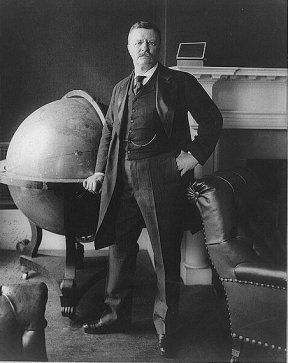
\includegraphics[width=0.6\textwidth]{teddy_roosevelt_portrait1.jpg}\end{figure}
{\em At the end of Theodore Roosevelt's second term in office, he set out to tour Africa and Europe, hoping to allow his successor, President Taft, to step into the enormous shoes TR had left and become his own man. After a safari in Africa, he traveled throughout Europe. While in France, he was invited to speak at the historic University of Paris. Roosevelt used the opportunity to deliver a powerful address on the requirements of citizenship, the characteristics which would keep democracies like France and the United States robust and strong. This speech is famous for the “man in the arena” quote, but the entire speech is an absolute must read.}

\vspace{10 mm}

Strange and impressive associations rise in the mind of a man from the New World who speaks before this august body in this ancient institution of learning. Before his eyes pass the shadows of mighty kings and war-like nobles, of great masters of law and theology; through the shining dust of the dead centuries he sees crowded figures that tell of the power and learning and splendor of times gone by; and he sees also the innumerable host of humble students to whom clerkship meant emancipation, to whom it was well-nigh the only outlet from the dark thraldom of the Middle Ages.

This was the most famous university of mediaeval Europe at a time when no one dreamed that there was a New World to discover. Its services to the cause of human knowledge already stretched far back into the remote past at a time when my forefathers, three centuries ago, were among the sparse bands of traders, ploughmen, wood-choppers, and fisherfolk who, in hard struggle with the iron unfriendliness of the Indian-haunted land, were laying the foundations of what has now become the giant republic of the West. To conquer a continent, to tame the shaggy roughness of wild nature, means grim warfare; and the generations engaged in it cannot keep, still less add to, the stores of garnered wisdom which where once theirs, and which are still in the hands of their brethren who dwell in the old land. To conquer the wilderness means to wrest victory from the same hostile forces with which mankind struggled on the immemorial infancy of our race. The primaeval conditions must be met by the primaeval qualities which are incompatible with the retention of much that has been painfully acquired by humanity as through the ages it has striven upward toward civilization. In conditions so primitive there can be but a primitive culture. At first only the rudest school can be established, for no others would meet the needs of the hard-driven, sinewy folk who thrust forward the frontier in the teeth of savage men and savage nature; and many years elapse before any of these schools can develop into seats of higher learning and broader culture.

The pioneer days pass; the stump-dotted clearings expand into vast stretches of fertile farm land; the stockaded clusters of log cabins change into towns; the hunters of game, the fellers of trees, the rude frontier traders and tillers of the soil, the men who wander all their lives long through the wilderness as the heralds and harbingers of an oncoming civilization, themselves vanish before the civilization for which they have prepared the way. The children of their successors and supplanters, and then their children and their children and children's children, change and develop with extraordinary rapidity. The conditions accentuate vices and virtues, energy and ruthlessness, all the good qualities and all the defects of an intense individualism, self-reliant, self-centered, far more conscious of its rights than of its duties, and blind to its own shortcomings. To the hard materialism of the frontier days succeeds the hard materialism of an industrialism even more intense and absorbing than that of the older nations; although these themselves have likewise already entered on the age of a complex and predominantly industrial civilization.

As the country grows, its people, who have won success in so many lines, turn back to try to recover the possessions of the mind and the spirit, which perforce their fathers threw aside in order better to wage the first rough battles for the continent their children inherit. The leaders of thought and of action grope their way forward to a new life, realizing, sometimes dimly, sometimes clear-sightedly, that the life of material gain, whether for a nation or an individual, is of value only as a foundation, only as there is added to it the uplift that comes from devotion to loftier ideals. The new life thus sought can in part be developed afresh from what is roundabout in the New World; but it can developed in full only by freely drawing upon the treasure-houses of the Old World, upon the treasures stored in the ancient abodes of wisdom and learning, such as this is where I speak to-day. It is a mistake for any nation to merely copy another; but it is even a greater mistake, it is a proof of weakness in any nation, not to be anxious to learn from one another and willing and able to adapt that learning to the new national conditions and make it fruitful and productive therein. It is for us of the New World to sit at the feet of Gamaliel of the Old; then, if we have the right stuff in us, we can show that Paul in his turn can become a teacher as well as a scholar.

To-day I shall speak to you on the subject of individual citizenship, the one subject of vital importance to you, my hearers, and to me and my countrymen, because you and we a great citizens of great democratic republics. A democratic republic such as ours – an effort to realize its full sense government by, of, and for the people – represents the most gigantic of all possible social experiments, the one fraught with great responsibilities alike for good and evil. The success or republics like yours and like ours means the glory, and our failure of despair, of mankind; and for you and for us the question of the quality of the individual citizen is supreme. Under other forms of government, under the rule of one man or very few men, the quality of the leaders is all-important. If, under such governments, the quality of the rulers is high enough, then the nations for generations lead a brilliant career, and add substantially to the sum of world achievement, no matter how low the quality of average citizen; because the average citizen is an almost negligible quantity in working out the final results of that type of national greatness.

But with you and us the case is different. With you here, and with us in my own home, in the long run, success or failure will be conditioned upon the way in which the average man, the average women, does his or her duty, first in the ordinary, every-day affairs of life, and next in those great occasional cries which call for heroic virtues. The average citizen must be a good citizen if our republics are to succeed. The stream will not permanently rise higher than the main source; and the main source of national power and national greatness is found in the average citizenship of the nation. Therefore it behooves us to do our best to see that the standard of the average citizen is kept high; and the average cannot be kept high unless the standard of the leaders is very much higher.

It is well if a large proportion of the leaders in any republic, in any democracy, are, as a matter of course, drawn from the classes represented in this audience to-day; but only provided that those classes possess the gifts of sympathy with plain people and of devotion to great ideals. You and those like you have received special advantages; you have all of you had the opportunity for mental training; many of you have had leisure; most of you have had a chance for enjoyment of life far greater than comes to the majority of your fellows. To you and your kind much has been given, and from you much should be expected. Yet there are certain failings against which it is especially incumbent that both men of trained and cultivated intellect, and men of inherited wealth and position should especially guard themselves, because to these failings they are especially liable; and if yielded to, their – your – chances of useful service are at an end.

Let the man of learning, the man of lettered leisure, beware of that queer and cheap temptation to pose to himself and to others as a cynic, as the man who has outgrown emotions and beliefs, the man to whom good and evil are as one. The poorest way to face life is to face it with a sneer. There are many men who feel a kind of twister pride in cynicism; there are many who confine themselves to criticism of the way others do what they themselves dare not even attempt. There is no more unhealthy being, no man less worthy of respect, than he who either really holds, or feigns to hold, an attitude of sneering disbelief toward all that is great and lofty, whether in achievement or in that noble effort which, even if it fails, comes to second achievement. A cynical habit of thought and speech, a readiness to criticise work which the critic himself never tries to perform, an intellectual aloofness which will not accept contact with life's realities – all these are marks, not as the possessor would fain to think, of superiority but of weakness. They mark the men unfit to bear their part painfully in the stern strife of living, who seek, in the affection of contempt for the achievements of others, to hide from others and from themselves in their own weakness. The rule is easy; there is none easier, save only the rule of the man who sneers alike at both criticism and performance.

It is not the critic who counts; not the man who points out how the strong man stumbles, or where the doer of deeds could have done them better. The credit belongs to the man who is actually in the arena, whose face in marred by dust and sweat and blood; who strives valiantly; who errs, who comes short again and again, because there is no effort without error and shortcoming; but who does actually strive to do the deeds; who knows great enthusiasms, the great devotions; who spends himself in a worthy cause; who at the best knows in the end the triumph of high achievement, and who at the worst, if he fails, at least fails while daring greatly, so that his place shall never be with those cold and timid souls who neither know victory nor defeat. Shame on the man of cultivated taste who permits refinement to develop into fastidiousness that unfits him for doing the rough work of a workaday world. Among the free peoples who govern themselves there is but a small field of usefulness open for the men of cloistered life who shrink from contact with their fellows. Still less room is there for those who deride of slight what is done by those who actually bear the brunt of the day; nor yet for those others who always profess that they would like to take action, if only the conditions of life were not exactly what they actually are. The man who does nothing cuts the same sordid figure in the pages of history, whether he be a cynic, or fop, or voluptuary. There is little use for the being whose tepid soul knows nothing of great and generous emotion, of the high pride, the stern belief, the lofty enthusiasm, of the men who quell the storm and ride the thunder. Well for these men if they succeed; well also, though not so well, if they fail, given only that they have nobly ventured, and have put forth all their heart and strength. It is war-worn Hotspur, spent with hard fighting, he of the many errors and valiant end, over whose memory we love to linger, not over the memory of the young lord who “but for the vile guns would have been a valiant soldier.”

France has taught many lessons to other nations: surely one of the most important lesson is the lesson her whole history teaches, that a high artistic and literary development is compatible with notable leadership im arms and statecraft. The brilliant gallantry of the French soldier has for many centuries been proverbial; and during these same centuries at every court in Europe the “freemasons of fashion: have treated the French tongue as their common speech; while every artist and man of letters, and every man of science able to appreciate that marvelous instrument of precision, French prose, had turned toward France for aid and inspiration. How long the leadership in arms and letters has lasted is curiously illustrated by the fact that the earliest masterpiece in a modern tongue is the splendid French epic which tells of Roland's doom and the vengeance of Charlemange when the lords of the Frankish hosts where stricken at Roncesvalles.

Let those who have, keep, let those who have not, strive to attain, a high standard of cultivation and scholarship. Yet let us remember that these stand second to certain other things. There is need of a sound body, and even more of a sound mind. But above mind and above body stands character – the sum of those qualities which we mean when we speak of a man's force and courage, of his good faith and sense of honor. I believe in exercise for the body, always provided that we keep in mind that physical development is a means and not an end. I believe, of course, in giving to all the people a good education. But the education must contain much besides book-learning in order to be really good. We must ever remember that no keenness and subtleness of intellect, no polish, no cleverness, in any way make up for the lack of the great solid qualities. Self restraint, self mastery, common sense, the power of accepting individual responsibility and yet of acting in conjunction with others, courage and resolution – these are the qualities which mark a masterful people. Without them no people can control itself, or save itself from being controlled from the outside. I speak to brilliant assemblage; I speak in a great university which represents the flower of the highest intellectual development; I pay all homage to intellect and to elaborate and specialized training of the intellect; and yet I know I shall have the assent of all of you present when I add that more important still are the commonplace, every-day qualities and virtues.

Such ordinary, every-day qualities include the will and the power to work, to fight at need, and to have plenty of healthy children. The need that the average man shall work is so obvious as hardly to warrant insistence. There are a few people in every country so born that they can lead lives of leisure. These fill a useful function if they make it evident that leisure does not mean idleness; for some of the most valuable work needed by civilization is essentially non-remunerative in its character, and of course the people who do this work should in large part be drawn from those to whom remuneration is an object of indifference. But the average man must earn his own livelihood. He should be trained to do so, and he should be trained to feel that he occupies a contemptible position if he does not do so; that he is not an object of envy if he is idle, at whichever end of the social scale he stands, but an object of contempt, an object of derision.

In the next place, the good man should be both a strong and a brave man; that is, he should be able to fight, he should be able to serve his country as a soldier, if the need arises. There are well-meaning philosophers who declaim against the unrighteousness of war. They are right only if they lay all their emphasis upon the unrighteousness. War is a dreadful thing, and unjust war is a crime against humanity. But it is such a crime because it is unjust, not because it is a war. The choice must ever be in favor of righteousness, and this is whether the alternative be peace or whether the alternative be war. The question must not be merely, Is there to be peace or war? The question must be, Is it right to prevail? Are the great laws of righteousness once more to be fulfilled? And the answer from a strong and virile people must be “Yes,” whatever the cost. Every honorable effort should always be made to avoid war, just as every honorable effort should always be made by the individual in private life to keep out of a brawl, to keep out of trouble; but no self-respecting individual, no self-respecting nation, can or ought to submit to wrong.

Finally, even more important than ability to work, even more important than ability to fight at need, is it to remember that chief of blessings for any nations is that it shall leave its seed to inherit the land. It was the crown of blessings in Biblical times and it is the crown of blessings now. The greatest of all curses in is the curse of sterility, and the severest of all condemnations should be that visited upon willful sterility. The first essential in any civilization is that the man and women shall be father and mother of healthy children, so that the race shall increase and not decrease. If that is not so, if through no fault of the society there is failure to increase, it is a great misfortune. If the failure is due to the deliberate and wilful fault, then it is not merely a misfortune, it is one of those crimes of ease and self-indulgence, of shrinking from pain and effort and risk, which in the long run Nature punishes more heavily than any other. If we of the great republics, if we, the free people who claim to have emancipated ourselves form the thraldom of wrong and error, bring down on our heads the curse that comes upon the willfully barren, then it will be an idle waste of breath to prattle of our achievements, to boast of all that we have done. No refinement of life, no delicacy of taste, no material progress, no sordid heaping up riches, no sensuous development of art and literature, can in any way compensate for the loss of the great fundamental virtues; and of these great fundamental virtues the greatest is the race's power to perpetuate the race.

Character must show itself in the man's performance both of the duty he owes himself and of the duty he owes the state. The man's foremast duty is owed to himself and his family; and he can do this duty only by earning money, by providing what is essential to material well-being; it is only after this has been done that he can hope to build a higher superstructure on the solid material foundation; it is only after this has been done that he can help in his movements for the general well-being. He must pull his own weight first, and only after this can his surplus strength be of use to the general public. It is not good to excite that bitter laughter which expresses contempt; and contempt is what we feel for the being whose enthusiasm to benefit mankind is such that he is a burden to those nearest him; who wishes to do great things for humanity in the abstract, but who cannot keep his wife in comfort or educate his children.

Nevertheless, while laying all stress on this point, while not merely acknowledging but insisting upon the fact that there must be a basis of material well-being for the individual as for the nation, let us with equal emphasis insist that this material well-being represents nothing but the foundation, and that the foundation, though indispensable, is worthless unless upon it is raised the superstructure of a higher life. That is why I decline to recognize the mere multimillionaire, the man of mere wealth, as an asset of value to any country; and especially as not an asset to my own country. If he has earned or uses his wealth in a way that makes him a real benefit, of real use – and such is often the case – why, then he does become an asset of real worth. But it is the way in which it has been earned or used, and not the mere fact of wealth, that entitles him to the credit. There is need in business, as in most other forms of human activity, of the great guiding intelligences. Their places cannot be supplied by any number of lesser intelligences. It is a good thing that they should have ample recognition, ample reward. But we must not transfer our admiration to the reward instead of to the deed rewarded; and if what should be the reward exists without the service having been rendered, then admiration will only come from those who are mean of soul. The truth is that, after a certain measure of tangible material success or reward has been achieved, the question of increasing it becomes of constantly less importance compared to the other things that can be done in life. It is a bad thing for a nation to raise and to admire a false standard of success; and their can be no falser standard than that set by the deification of material well-being in and for itself. But the man who, having far surpassed the limits of providing for the wants; both of the body and mind, of himself and of those depending upon him, then piles up a great fortune, for the acquisition or retention of which he returns no corresponding benefit to the nation as a whole, should himself be made to feel that, so far from being desirable, he is an unworthy, citizen of the community: that he is to be neither admired nor envied; that his right-thinking fellow countrymen put him low in the scale of citizenship, and leave him to be consoled by the admiration of those whose level of purpose is even lower than his own.

My position as regards the moneyed interests can be put in a few words. In every civilized society property rights must be carefully safeguarded; ordinarily, and in the great majority of cases, human rights and property rights are fundamentally and in the long run identical; but when it clearly appears that there is a real conflict between them, human rights must have the upper hand, for property belongs to man and not man to property.

In fact, it is essential to good citizenship clearly to understand that there are certain qualities which we in a democracy are prone to admire in and of themselves, which ought by rights to be judged admirable or the reverse solely from the standpoint of the use made of them. Foremost among these I should include two very distinct gifts – the gift of money-making and the gift of oratory. Money-making, the money touch I have spoken of above. It is a quality which in a moderate degree is essential. It may be useful when developed to a very great degree, but only if accompanied and controlled by other qualities; and without such control the possessor tends to develop into one of the least attractive types produced by a modern industrial democracy. So it is with the orator. It is highly desirable that a leader of opinion in democracy should be able to state his views clearly and convincingly. But all that the oratory can do of value to the community is enable the man thus to explain himself; if it enables the orator to put false values on things, it merely makes him power for mischief. Some excellent public servants have not that gift at all, and must merely rely on their deeds to speak for them; and unless oratory does represent genuine conviction based on good common sense and able to be translated into efficient performance, then the better the oratory the greater the damage to the public it deceives. Indeed, it is a sign of marked political weakness in any commonwealth if the people tend to be carried away by mere oratory, if they tend to value words in and for themselves, as divorced from the deeds for which they are supposed to stand. The phrase-maker, the phrase-monger, the ready talker, however great his power, whose speech does not make for courage, sobriety, and right understanding, is simply a noxious element in the body politic, and it speaks ill for the public if he has influence over them. To admire the gift of oratory without regard to the moral quality behind the gift is to do wrong to the republic.

Of course all that I say of the orator applies with even greater force to the orator's latter-day and more influential brother, the journalist. The power of the journalist is great, but he is entitled neither to respect nor admiration because of that power unless it is used aright. He cna do, and often does, great good. He can do, and he often does, infinite mischief. All journalists, all writers, for the very reason that they appreciate the vast possibilities of their profession, should bear testimony against those who deeply discredit it. Offenses against taste and morals, which are bad enough in a private citizen, are infinitely worse if made into instruments for debauching the community through a newspaper. Mendacity, slander, sensationalism, inanity, vapid triviality, all are potent factors for the debauchery of the public mind and conscience. The excuse advanced for vicious writing, that the public demands it and that demand must be supplied, can no more be admitted than if it were advanced by purveyors of food who sell poisonous adulterations.

In short, the good citizen in a republic must realize that the ought to possess two sets of qualities, and that neither avails without the other. He must have those qualities which make for efficiency; and that he also must have those qualities which direct the efficiency into channels for the public good. He is useless if he is inefficient. There is nothing to be done with that type of citizen of whom all that can be said is that he is harmless. Virtue which is dependant upon a sluggish circulation is not impressive. There is little place in active life for the timid good man. The man who is saved by weakness from robust wickedness is likewise rendered immune from robuster virtues. The good citizen in a republic must first of all be able to hold his own. He is no good citizen unless he has the ability which will make him work hard and which at need will make him fight hard. The good citizen is not a good citizen unless he is an efficient citizen.

But if a man's efficiency is not guided and regulated by a moral sense, then the more efficient he is the worse he is, the more dangerous to the body politic. Courage, intellect, all the masterful qualities, serve but to make a man more evil if they are merely used for that man's own advancement, with brutal indifference to the rights of others. It speaks ill for the community if the community worships these qualities and treats their possessors as heroes regardless of whether the qualities are used rightly or wrongly. It makes no difference as to the precise way in which this sinister efficiency is shown. It makes no difference whether such a man's force and ability betray themselves in a career of money-maker or politician, soldier or orator, journalist or popular leader. If the man works for evil, then the more successful he is the more he should be despised and condemned by all upright and far-seeing men. To judge a man merely by success is an abhorrent wrong; and if the people at large habitually so judge men, if they grow to condone wickedness because the wicked man triumphs, they show their inability to understand that in the last analysis free institutions rest upon the character of citizenship, and that by such admiration of evil they prove themselves unfit for liberty.

The homely virtues of the household, the ordinary workaday virtues which make the woman a good housewife and housemother, which make the man a hard worker, a good husband and father, a good soldier at need, stand at the bottom of character. But of course many other must be added thereto if a state is to be not only free but great. Good citizenship is not good citizenship if only exhibited in the home. There remains the duties of the individual in relation to the State, and these duties are none too easy under the conditions which exist where the effort is made to carry on the free government in a complex industrial civilization. Perhaps the most important thing the ordinary citizen, and, above all, the leader of ordinary citizens, has to remember in political life is that he must not be a sheer doctrinaire. The closest philosopher, the refined and cultured individual who from his library tells how men ought to be governed under ideal conditions, is of no use in actual governmental work; and the one-sided fanatic, and still more the mob-leader, and the insincere man who to achieve power promises what by no possibility can be performed, are not merely useless but noxious.

The citizen must have high ideals, and yet he must be able to achieve them in practical fashion. No permanent good comes from aspirations so lofty that they have grown fantastic and have become impossible and indeed undesirable to realize. The impractical visionary is far less often the guide and precursor than he is the embittered foe of the real reformer, of the man who, with stumblings and shortcoming, yet does in some shape, in practical fashion, give effect to the hopes and desires of those who strive for better things. Woe to the empty phrase-maker, to the empty idealist, who, instead of making ready the ground for the man of action, turns against him when he appears and hampers him when he does work! Moreover, the preacher of ideals must remember how sorry and contemptible is the figure which he will cut, how great the damage that he will do, if he does not himself, in his own life, strive measurably to realize the ideals that he preaches for others. Let him remember also that the worth of the ideal must be largely determined by the success with which it can in practice be realized. We should abhor the so-called “practical” men whose practicality assumes the shape of that peculiar baseness which finds its expression in disbelief in morality and decency, in disregard of high standards of living and conduct. Such a creature is the worst enemy of the body of politic. But only less desirable as a citizen is his nominal opponent and real ally, the man of fantastic vision who makes the impossible better forever the enemy of the possible good.

We can just as little afford to follow the doctrinaires of an extreme individualism as the doctrinaires of an extreme socialism. Individual initiative, so far from being discouraged, should be stimulated; and yet we should remember that, as society develops and grows more complex, we continually find that things which once it was desirable to leave to individual initiative can, under changed conditions, be performed with better results by common effort. It is quite impossible, and equally undesirable, to draw in theory a hard-and-fast line which shall always divide the two sets of cases. This every one who is not cursed with the pride of the closest philosopher will see, if he will only take the trouble to think about some of our closet phenomena. For instance, when people live on isolated farms or in little hamlets, each house can be left to attend to its own drainage and water-supply; but the mere multiplication of families in a given area produces new problems which, because they differ in size, are found to differ not only in degree, but in kind from the old; and the questions of drainage and water-supply have to be considered from the common standpoint. It is not a matter for abstract dogmatizing to decide when this point is reached; it is a matter to be tested by practical experiment. Much of the discussion about socialism and individualism is entirely pointless, because of the failure to agree on terminology. It is not good to be a slave of names. I am a strong individualist by personal habit, inheritance, and conviction; but it is a mere matter of common sense to recognize that the State, the community, the citizens acting together, can do a number of things better than if they were left to individual action. The individualism which finds its expression in the abuse of physical force is checked very early in the growth of civilization, and we of to-day should in our turn strive to shackle or destroy that individualism which triumphs by greed and cunning, which exploits the weak by craft instead of ruling them by brutality. We ought to go with any man in the effort to bring about justice and the equality of opportunity, to turn the tool-user more and more into the tool-owner, to shift burdens so that they can be more equitably borne. The deadening effect on any race of the adoption of a logical and extreme socialistic system could not be overstated; it would spell sheer destruction; it would produce grosser wrong and outrage, fouler immortality, than any existing system. But this does not mean that we may not with great advantage adopt certain of the principles professed by some given set of men who happen to call themselves Socialists; to be afraid to do so would be to make a mark of weakness on our part.

But we should not take part in acting a lie any more than in telling a lie. We should not say that men are equal where they are not equal, nor proceed upon the assumption that there is an equality where it does not exist; but we should strive to bring about a measurable equality, at least to the extent of preventing the inequality which is due to force or fraud. Abraham Lincoln, a man of the plain people, blood of their blood, and bone of their bone, who all his life toiled and wrought and suffered for them, at the end died for them, who always strove to represent them, who would never tell an untruth to or for them, spoke of the doctrine of equality with his usual mixture of idealism and sound common sense. He said (I omit what was of merely local significance):

\begin{quote}“I think the authors of the Declaration of Independence intended to include all men, but they did not mean to declare all men equal in all respects. They did not mean to say all men were equal in color, size, intellect, moral development or social capacity. They defined with tolerable distinctness in what they did consider all men created equal-equal in certain inalienable rights, among which are life, liberty and pursuit of happiness. This they said, and this they meant. They did not mean to assert the obvious untruth that all were actually enjoying that equality, or yet that they were about to confer it immediately upon them. They meant to set up a standard maxim for free society which should be familiar to all – constantly looked to, constantly labored for, and, even though never perfectly attained, constantly approximated, and thereby constantly spreading and deepening its influence, and augmenting the happiness and value of life to all people, everywhere.”\end{quote}

We are bound in honor to refuse to listen to those men who would make us desist from the effort to do away with the inequality which means injustice; the inequality of right, opportunity, of privilege. We are bound in honor to strive to bring ever nearer the day when, as far is humanly possible, we shall be able to realize the ideal that each man shall have an equal opportunity to show the stuff that is in him by the way in which he renders service. There should, so far as possible, be equal of opportunity to render service; but just so long as there is inequality of service there should and must be inequality of reward. We may be sorry for the general, the painter, the artists, the worker in any profession or of any kind, whose misfortune rather than whose fault it is that he does his work ill. But the reward must go to the man who does his work well; for any other course is to create a new kind of privilege, the privilege of folly and weakness; and special privilege is injustice, whatever form it takes.

To say that the thriftless, the lazy, the vicious, the incapable, ought to have reward given to those who are far-sighted, capable, and upright, is to say what is not true and cannot be true. Let us try to level up, but let us beware of the evil of leveling down. If a man stumbles, it is a good thing to help him to his feet. Every one of us needs a helping hand now and then. But if a man lies down, it is a waste of time to try and carry him; and it is a very bad thing for every one if we make men feel that the same reward will come to those who shirk their work and those who do it.

Let us, then, take into account the actual facts of life, and not be misled into following any proposal for achieving the millennium, for recreating the golden age, until we have subjected it to hardheaded examination. On the other hand, it is foolish to reject a proposal merely because it is advanced by visionaries. If a given scheme is proposed, look at it on its merits, and, in considering it, disregard formulas. It does not matter in the least who proposes it, or why. If it seems good, try it. If it proves good, accept it; otherwise reject it. There are plenty of good men calling themselves Socialists with whom, up to a certain point, it is quite possible to work. If the next step is one which both we and they wish to take, why of course take it, without any regard to the fact that our views as to the tenth step may differ. But, on the other hand, keep clearly in mind that, though it has been worth while to take one step, this does not in the least mean that it may not be highly disadvantageous to take the next. It is just as foolish to refuse all progress because people demanding it desire at some points to go to absurd extremes, as it would be to go to these absurd extremes simply because some of the measures advocated by the extremists were wise.

The good citizen will demand liberty for himself, and as a matter of pride he will see to it that others receive liberty which he thus claims as his own. Probably the best test of true love of liberty in any country in the way in which minorities are treated in that country. Not only should there be complete liberty in matters of religion and opinion, but complete liberty for each man to lead his life as he desires, provided only that in so he does not wrong his neighbor. Persecution is bad because it is persecution, and without reference to which side happens at the most to be the persecutor and which the persecuted. Class hatred is bad in just the same way, and without regard to the individual who, at a given time, substitutes loyalty to a class for loyalty to a nation, of substitutes hatred of men because they happen to come in a certain social category, for judgement awarded them according to their conduct. Remember always that the same measure of condemnation should be extended to the arrogance which would look down upon or crush any man because he is poor and to envy and hatred which would destroy a man because he is wealthy. The overbearing brutality of the man of wealth or power, and the envious and hateful malice directed against wealth or power, are really at root merely different manifestations of the same quality, merely two sides of the same shield. The man who, if born to wealth and power, exploits and ruins his less fortunate brethren is at heart the same as the greedy and violent demagogue who excites those who have not property to plunder those who have. The gravest wrong upon his country is inflicted by that man, whatever his station, who seeks to make his countrymen divide primarily in the line that separates class from class, occupation from occupation, men of more wealth from men of less wealth, instead of remembering that the only safe standard is that which judges each man on his worth as a man, whether he be rich or whether he be poor, without regard to his profession or to his station in life. Such is the only true democratic test, the only test that can with propriety be applied in a republic. There have been many republics in the past, both in what we call antiquity and in what we call the Middle Ages. They fell, and the prime factor in their fall was the fact that the parties tended to divide along the wealth that separates wealth from poverty. It made no difference which side was successful; it made no difference whether the republic fell under the rule of and oligarchy or the rule of a mob. In either case, when once loyalty to a class had been substituted for loyalty to the republic, the end of the republic was at hand. There is no greater need to-day than the need to keep ever in mind the fact that the cleavage between right and wrong, between good citizenship and bad citizenship, runs at right angles to, and not parallel with, the lines of cleavage between class and class, between occupation and occupation. Ruin looks us in the face if we judge a man by his position instead of judging him by his conduct in that position.

In a republic, to be successful we must learn to combine intensity of conviction with a broad tolerance of difference of conviction. Wide differences of opinion in matters of religious, political, and social belief must exist if conscience and intellect alike are not be stunted, if there is to be room for healthy growth. Bitter internecine hatreds, based on such differences, are signs, not of earnestness of belief, but of that fanaticism which, whether religious or antireligious, democratic or antidemocratic, it itself but a manifestation of the gloomy bigotry which has been the chief factor in the downfall of so many, many nations.

Of one man in especial, beyond any one else, the citizens of a republic should beware, and that is of the man who appeals to them to support him on the ground that he is hostile to other citizens of the republic, that he will secure for those who elect him, in one shape or another, profit at the expense of other citizens of the republic. It makes no difference whether he appeals to class hatred or class interest, to religious or antireligious prejudice. The man who makes such an appeal should always be presumed to make it for the sake of furthering his own interest. The very last thing an intelligent and self-respecting member of a democratic community should do is to reward any public man because that public man says that he will get the private citizen something to which this private citizen is not entitled, or will gratify some emotion or animosity which this private citizen ought not to possess. Let me illustrate this by one anecdote from my own experience. A number of years ago I was engaged in cattle-ranching on the great plains of the western Unite States. There were no fences. The cattle wandered free, the ownership of each one was determined by the brand; the calves were branded with the brand of the cows they followed. If on a round-up and animal was passed by, the following year it would appear as an unbranded yearling, and was then called a maverick. By the custom of the country these mavericks were branded with the brand of the man on whose range they were found. One day I was riding the range with a newly hired cowboy, and we came upon a maverick. We roped and threw it; then we built a fire, took out a cinch-ring, heated it in the fire; and then the cowboy started to put on the brand. I said to him, “It So-and-so's brand,” naming the man on whose range we happened to be. He answered: “That's all right, boss; I know my business.” In another moment I said to him: “Hold on, you are putting on my brand!” To which he answered: “That's all right; I always put on the boss's brand.” I answered: “Oh, very well. Now you go straight back to the ranch and get whatever is owing to you; I don't need you any longer.” He jumped up and said: “Why, what's the matter? I was putting on your brand.” And I answered: “Yes, my friend, and if you will steal for me then you will steal from me.”

Now, the same principle which applies in private life applies also in public life. If a public man tries to get your vote by saying that he will do something wrong in your interest, you can be absolutely certain that if ever it becomes worth his while he will do something wrong against your interest.

So much for the citizenship to the individual in his relations to his family, to his neighbor, to the State. There remain duties of citizenship which the State, the aggregation of all the individuals, owes in connection with other States, with other nations. Let me say at once that I am no advocate of a foolish cosmopolitanism. I believe that a man must be a good patriot before he can be, and as the only possible way of being, a good citizen of the world. Experience teaches us that the average man who protests that his international feeling swamps his national feeling, that he does not care for his country because he cares so much for mankind, in actual practice proves himself the foe of mankind; that the man who says that he does not care to be a citizen of any one country, because he is the citizen of the world, is in fact usually and exceedingly undesirable citizen of whatever corner of the world he happens at the moment to be in. In the dim future all moral needs and moral standards may change; but at present, if a man can view his own country and all others countries from the same level with tepid indifference, it is wise to distrust him, just as it is wise to distrust the man who can take the same dispassionate view of his wife and mother. However broad and deep a man's sympathies, however intense his activities, he need have no fear that they will be cramped by love of his native land.

Now, this does not mean in the least that a man should not wish to good outside of his native land. On the contrary, just as I think that the man who loves his family is more apt to be a good neighbor than the man who does not, so I think that the most useful member of the family of nations is normally a strongly patriotic nation. So far from patriotism being inconsistent with a proper regard for the rights of other nations, I hold that the true patriot, who is as jealous of the national honor as a gentleman of his own honor, will be careful to see that the nations neither inflicts nor suffers wrong, just as a gentleman scorns equally to wrong others or to suffer others to wrong him. I do not for one moment admit that a man should act deceitfully as a public servant in his dealing with other nations, any more than he should act deceitfully in his dealings as a private citizen with other private citizens. I do not for one moment admit that a nation should treat other nations in a different spirit from that in which an honorable man would treat other men.

In practically applying this principle to the two sets of cases there is, of course, a great practical difference to be taken into account. We speak of international law; but international law is something wholly different from private of municipal law, and the capital difference is that there is a sanction for the one and no sanction for the other; that there is an outside force which compels individuals to obey the one, while there is no such outside force to compel obedience as regards to the other. International law will, I believe, as the generations pass, grow stronger and stronger until in some way or other there develops the power to make it respected. But as yet it is only in the first formative period. As yet, as a rule, each nation is of necessity to judge for itself in matters of vital importance between it and its neighbors, and actions must be of necessity, where this is the case, be different from what they are where, as among private citizens, there is an outside force whose action is all-powerful and must be invoked in any crisis of importance. It is the duty of wise statesman, gifted with the power of looking ahead, to try to encourage and build up every movement which will substitute or tend to substitute some other agency for force in the settlement of international disputes. It is the duty of every honest statesman to try to guide the nation so that it shall not wrong any other nation. But as yet the great civilized peoples, if they are to be true to themselves and to the cause of humanity and civilization, must keep in mind that in the last resort they must possess both the will and the power to resent wrong-doings from others. The men who sanely believe in a lofty morality preach righteousness; but they do not preach weakness, whether among private citizens or among nations. We believe that our ideals should be so high, but not so high as to make it impossible measurably to realize them. We sincerely and earnestly believe in peace; but if peace and justice conflict, we scorn the man who would not stand for justice though the whole world came in arms against him.

And now, my hosts, a word in parting. You and I belong to the only two republics among the great powers of the world. The ancient friendship between France and the United States has been, on the whole, a sincere and disinterested friendship. A calamity to you would be a sorrow to us. But it would be more than that. In the seething turmoil of the history of humanity certain nations stand out as possessing a peculiar power or charm, some special gift of beauty or wisdom of strength, which puts them among the immortals, which makes them rank forever with the leaders of mankind. France is one of these nations. For her to sink would be a loss to all the world. There are certain lessons of brilliance and of generous gallantry that she can teach better than any of her sister nations. When the French peasantry sang of Malbrook, it was to tell how the soul of this warrior-foe took flight upward through the laurels he had won. Nearly seven centuries ago, Froisart, writing of the time of dire disaster, said that the realm of France was never so stricken that there were not left men who would valiantly fight for it. You have had a great past. I believe you will have a great future. Long may you carry yourselves proudly as citizens of a nation which bears a leading part in the teaching and uplifting of mankind.


\chapter{Franklin Delano Roosevelt - First Inaugural Address}

\textbf{\Large{Washington D.C. -- March 04, 1933 }}

\vspace{10 mm}

\begin{figure}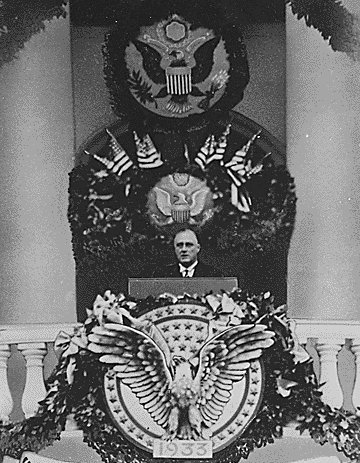
\includegraphics[width=0.6\textwidth]{fdr-first-inaug.jpg}\end{figure}
{\em Franklin Delano Roosevelt handily beat incumbent Herbert Hoover in the 1932 presidential election. The country was deep into the Great Depression, and the public felt that Hoover did not fully sympathize with their plight and was not doing enough to alleviate it. No one was quite clear on what FDR's plan was, but as in today's election season, “change” was enough of an idea to power a campaign. In his First Inaugural Address, Roosevelt sought to buoy up the injured psyche of the American people and present his case for why he would need broad executive powers to tackle the Depression.}

\vspace{10 mm}

President Hoover, Mr. Chief Justice, my friends:

This is a day of national consecration. And I am certain that on this day my fellow Americans expect that on my induction into the Presidency, I will address them with a candor and a decision which the present situation of our people impels.

This is preeminently the time to speak the truth, the whole truth, frankly and boldly. Nor need we shrink from honestly facing conditions in our country today. This great Nation will endure, as it has endured, will revive and will prosper.

So, first of all, let me assert my firm belief that the only thing we have to fear is fear itself — nameless, unreasoning, unjustified terror which paralyzes needed efforts to convert retreat into advance. In every dark hour of our national life, a leadership of frankness and of vigor has met with that understanding and support of the people themselves which is essential to victory. And I am convinced that you will again give that support to leadership in these critical days.

In such a spirit on my part and on yours we face our common difficulties. They concern, thank God, only material things. Values have shrunk to fantastic levels; taxes have risen; our ability to pay has fallen; government of all kinds is faced by serious curtailment of income; the means of exchange are frozen in the currents of trade; the withered leaves of industrial enterprise lie on every side; farmers find no markets for their produce; and the savings of many years in thousands of families are gone. More important, a host of unemployed citizens face the grim problem of existence, and an equally great number toil with little return. Only a foolish optimist can deny the dark realities of the moment.

And yet our distress comes from no failure of substance. We are stricken by no plague of locusts. Compared with the perils which our forefathers conquered, because they believed and were not afraid, we have still much to be thankful for. Nature still offers her bounty and human efforts have multiplied it. Plenty is at our doorstep, but a generous use of it languishes in the very sight of the supply.

Primarily, this is because the rulers of the exchange of mankind's goods have failed, through their own stubbornness and their own incompetence, have admitted their failure, and have abdicated. Practices of the unscrupulous money changers stand indicted in the court of public opinion, rejected by the hearts and minds of men.

True, they have tried. But their efforts have been cast in the pattern of an outworn tradition. Faced by failure of credit, they have proposed only the lending of more money. Stripped of the lure of profit by which to induce our people to follow their false leadership, they have resorted to exhortations, pleading tearfully for restored confidence. They only know the rules of a generation of self-seekers. They have no vision, and when there is no vision the people perish.

Yes, the money changers have fled from their high seats in the temple of our civilization. We may now restore that temple to the ancient truths. The measure of that restoration lies in the extent to which we apply social values more noble than mere monetary profit.

Happiness lies not in the mere possession of money; it lies in the joy of achievement, in the thrill of creative effort. The joy, the moral stimulation of work no longer must be forgotten in the mad chase of evanescent profits. These dark days, my friends, will be worth all they cost us if they teach us that our true destiny is not to be ministered unto but to minister to ourselves, to our fellow men.

Recognition of that falsity of material wealth as the standard of success goes hand in hand with the abandonment of the false belief that public office and high political position are to be valued only by the standards of pride of place and personal profit; and there must be an end to a conduct in banking and in business which too often has given to a sacred trust the likeness of callous and selfish wrongdoing. Small wonder that confidence languishes, for it thrives only on honesty, on honor, on the sacredness of obligations, on faithful protection, and on unselfish performance; without them it cannot live.

Restoration calls, however, not for changes in ethics alone. This Nation is asking for action, and action now.

Our greatest primary task is to put people to work. This is no unsolvable problem if we face it wisely and courageously. It can be accomplished in part by direct recruiting by the Government itself, treating the task as we would treat the emergency of a war, but at the same time, through this employment, accomplishing great — greatly needed projects to stimulate and reorganize the use of our great natural resources.

Hand in hand with that we must frankly recognize the overbalance of population in our industrial centers and, by engaging on a national scale in a redistribution, endeavor to provide a better use of the land for those best fitted for the land.

Yes, the task can be helped by definite efforts to raise the values of agricultural products, and with this the power to purchase the output of our cities. It can be helped by preventing realistically the tragedy of the growing loss through foreclosure of our small homes and our farms. It can be helped by insistence that the Federal, the State, and the local governments act forthwith on the demand that their cost be drastically reduced. It can be helped by the unifying of relief activities which today are often scattered, uneconomical, unequal. It can be helped by national planning for and supervision of all forms of transportation and of communications and other utilities that have a definitely public character. There are many ways in which it can be helped, but it can never be helped by merely talking about it.

We must act. We must act quickly.

And finally, in our progress towards a resumption of work, we require two safeguards against a return of the evils of the old order. There must be a strict supervision of all banking and credits and investments. There must be an end to speculation with other people's money. And there must be provision for an adequate but sound currency.

These, my friends, are the lines of attack. I shall presently urge upon a new Congress in special session detailed measures for their fulfillment, and I shall seek the immediate assistance of the 48 States.

Through this program of action we address ourselves to putting our own national house in order and making income balance outgo. Our international trade relations, though vastly important, are in point of time, and necessity, secondary to the establishment of a sound national economy. I favor, as a practical policy, the putting of first things first. I shall spare no effort to restore world trade by international economic readjustment; but the emergency at home cannot wait on that accomplishment.

The basic thought that guides these specific means of national recovery is not nationally — narrowly nationalistic. It is the insistence, as a first consideration, upon the interdependence of the various elements in and parts of the United States of America — a recognition of the old and permanently important manifestation of the American spirit of the pioneer. It is the way to recovery. It is the immediate way. It is the strongest assurance that recovery will endure.

In the field of world policy, I would dedicate this Nation to the policy of the good neighbor: the neighbor who resolutely respects himself and, because he does so, respects the rights of others; the neighbor who respects his obligations and respects the sanctity of his agreements in and with a world of neighbors.

If I read the temper of our people correctly, we now realize, as we have never realized before, our interdependence on each other; that we can not merely take, but we must give as well; that if we are to go forward, we must move as a trained and loyal army willing to sacrifice for the good of a common discipline, because without such discipline no progress can be made, no leadership becomes effective.

We are, I know, ready and willing to submit our lives and our property to such discipline, because it makes possible a leadership which aims at the larger good. This, I propose to offer, pledging that the larger purposes will bind upon us, bind upon us all as a sacred obligation with a unity of duty hitherto evoked only in times of armed strife.

With this pledge taken, I assume unhesitatingly the leadership of this great army of our people dedicated to a disciplined attack upon our common problems.

Action in this image, action to this end is feasible under the form of government which we have inherited from our ancestors. Our Constitution is so simple, so practical that it is possible always to meet extraordinary needs by changes in emphasis and arrangement without loss of essential form. That is why our constitutional system has proved itself the most superbly enduring political mechanism the modern world has ever seen.

It has met every stress of vast expansion of territory, of foreign wars, of bitter internal strife, of world relations. And it is to be hoped that the normal balance of executive and legislative authority may be wholly equal, wholly adequate to meet the unprecedented task before us. But it may be that an unprecedented demand and need for undelayed action may call for temporary departure from that normal balance of public procedure.

I am prepared under my constitutional duty to recommend the measures that a stricken nation in the midst of a stricken world may require. These measures, or such other measures as the Congress may build out of its experience and wisdom, I shall seek, within my constitutional authority, to bring to speedy adoption.

But, in the event that the Congress shall fail to take one of these two courses, in the event that the national emergency is still critical, I shall not evade the clear course of duty that will then confront me. I shall ask the Congress for the one remaining instrument to meet the crisis — broad Executive power to wage a war against the emergency, as great as the power that would be given to me if we were in fact invaded by a foreign foe.

For the trust reposed in me, I will return the courage and the devotion that befit the time. I can do no less.

We face the arduous days that lie before us in the warm courage of national unity; with the clear consciousness of seeking old and precious moral values; with the clean satisfaction that comes from the stern performance of duty by old and young alike. We aim at the assurance of a rounded, a permanent national life.

We do not distrust the — the future of essential democracy. The people of the United States have not failed. In their need they have registered a mandate that they want direct, vigorous action. They have asked for discipline and direction under leadership. They have made me the present instrument of their wishes. In the spirit of the gift I take it.

In this dedication — In this dedication of a Nation, we humbly ask the blessing of God.

May He protect each and every one of us.

May He guide me in the days to come.


\chapter{Lou Gehrig - Farewell to Baseball Address}

\textbf{\Large{Yankee Stadium -- June 04, 1939 }}

\vspace{10 mm}

\begin{figure}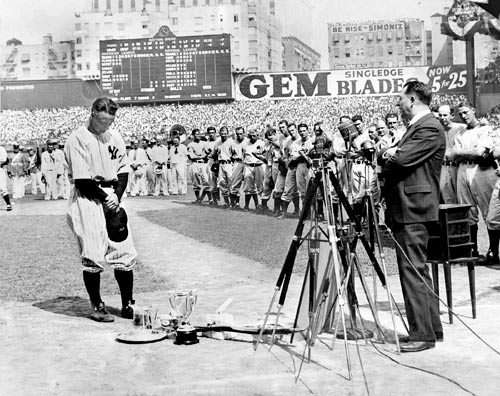
\includegraphics[width=0.6\textwidth]{gehrig_goodbye500.jpg}\end{figure}
{\em It seemed as if the luminous career of Lou Gehrig would go on forever. The Yankee's first baseman and prodigious slugger was nicknamed the Iron Horse for his durability and commitment to the game. Sadly, his record for suiting up for 2,130 consecutive games came to an end when at age 36, Gehrig was stricken with the crippling disease that now bears his name. On July 4, 1939, the Yankees held a ceremony to honor their teammate and friend. They retired Gehrig's number, spoke of his greatness, and presented him with various gifts, plaques, and trophies. When Gehrig finally addressed the crowd, he did not use the opportunity to wallow in pity. Instead, he spoke of the things he was grateful for and what a lucky guy he was.}

\vspace{10 mm}

Fans, for the past two weeks you have been reading about a bad break I got. Yet today I consider myself the luckiest man on the face of the earth. I have been in ballparks for seventeen years and have never received anything but kindness and encouragement from you fans.

Look at these grand men. Which of you wouldn't consider it the highlight of his career to associate with them for even one day?

Sure, I'm lucky. Who wouldn't consider it an honor to have known Jacob Ruppert – also the builder of baseball's greatest empire, Ed Barrow – to have spent the next nine years with that wonderful little fellow Miller Huggins – then to have spent the next nine years with that outstanding leader, that smart student of psychology – the best manager in baseball today, Joe McCarthy!

Sure, I'm lucky. When the New York Giants, a team you would give your right arm to beat, and vice versa, sends you a gift, that's something! When everybody down to the groundskeepers and those boys in white coats remember you with trophies, that's something.

When you have a wonderful mother-in-law who takes sides with you in squabbles against her own daughter, that's something. When you have a father and mother who work all their lives so that you can have an education and build your body, it's a blessing! When you have a wife who has been a tower of strength and shown more courage than you dreamed existed, that's the finest I know.

So I close in saying that I might have had a tough break – but I have an awful lot to live for!


\chapter{Winston Churchill - Blood, Sweat, and Tears}

\textbf{\Large{House of Commons, London -- May 13, 1940 }}

\vspace{10 mm}

\begin{figure}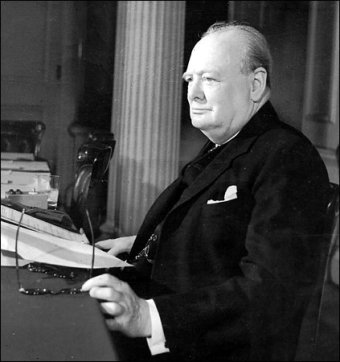
\includegraphics[width=0.6\textwidth]{winstonchurchillnytimes1.jpg}\end{figure}
{\em Winston Churchill's first speech to the House of Commons as Britain's new Prime Minister got off to an auspicious start. His welcome to that assembly was quite tepid, while outgoing PM Neville Chamberlain was enthusiastically applauded (the world did not yet know just how disastrous his appeasement policies would prove and did not trust Churchill). But Churchill's first speech, the first of three powerful oratories he gave during the Battle of France, would prove that England was in more than capable hands. A seemingly unstoppable Hitler was advancing rapidly across Europe, and Churchill wasted no time in calling his people to arms. While TR had actually been the first to utter the phrase, “blood, sweat and tears,” it was Churchill's use of these words that would leave an inedible and inspiring impression upon the world's mind.}

\vspace{10 mm}

Mr. Speaker:

On Friday evening last I received His Majesty's commission to form a new Administration. It was the evident wish and will of Parliament and the nation that this should be conceived on the broadest possible basis and that it should include all parties, both those who supported the late Government and also the parties of the Opposition.

I have completed the most important part of this task. A War Cabinet has been formed of five Members, representing, with the Liberal Opposition, the unity of the nation. The three party Leaders have agreed to serve, either in the War Cabinet or in high executive office. The three Fighting Services have been filled. It was necessary that this should be done in one single day, on account of the extreme urgency and rigour of events. A number of other key positions were filled yesterday, and I am submitting a further list to His Majesty tonight. I hope to complete the appointment of the principal Ministers during tomorrow. The appointment of the other Ministers usually takes a little longer, but I trust that, when Parliament meets again, this part of my task will be completed, and that the Administration will be complete in all respects.

Sir, I considered it in the public interest to suggest that the House should be summoned to meet today. Mr. Speaker agreed and took the necessary steps, in accordance with the powers conferred upon him by the Resolution of the House. At the end of the proceedings today, the Adjournment of the House will be proposed until Tuesday, the 21st May, with, of course, provision for earlier meeting, if need be. The business to be considered during that week will be notified to Members at the earliest opportunity. I now invite the House, by the Resolution which stands in my name, to record its approval of the steps taken and to declare its confidence in the new Government.

Sir, to form an Administration of this scale and complexity is a serious undertaking in itself, but it must be remembered that we are in the preliminary stage of one of the greatest battles in history, that we are in action at many points in Norway and in Holland, that we have to be prepared in the Mediterranean, that the air battle is continuous and that many preparations have to be made here at home. In this crisis I hope I may be pardoned if I do not address the House at any length today. I hope that any of my friends and colleagues, or former colleagues, who are affected by the political reconstruction, will make all allowances for any lack of ceremony with which it has been necessary to act. I would say to the House, as I said to those who've joined this government: “I have nothing to offer but blood, toil, tears and sweat.”

We have before us an ordeal of the most grievous kind. We have before us many, many long months of struggle and of suffering. You ask, what is our policy? I will say: It is to wage war, by sea, land and air, with all our might and with all the strength that God can give us; to wage war against a monstrous tyranny, never surpassed in the dark and lamentable catalogue of human crime. That is our policy. You ask, what is our aim? I can answer in one word: victory. Victory at all costs, victory in spite of all terror, victory, however long and hard the road may be; for without victory, there is no survival. Let that be realised; no survival for the British Empire, no survival for all that the British Empire has stood for, no survival for the urge and impulse of the ages, that mankind will move forward towards its goal.

But I take up my task with buoyancy and hope. I feel sure that our cause will not be suffered to fail among men. At this time I feel entitled to claim the aid of all, and I say, “Come then, let us go forward together with our united strength.”


\chapter{Winston Churchill - We Shall Fight on the Beaches}

\textbf{\Large{House of Commons, London -- June 04, 1940 }}

\vspace{10 mm}

\begin{figure}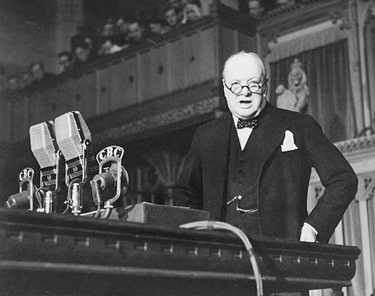
\includegraphics[width=0.6\textwidth]{wscparl.jpg}\end{figure}
{\em Winston Churchill, one of the greatest orators of the 20th century, was interestingly enough, like Demosthenes and other great orators before him, born with a speech impediment which he worked on until it no longer hindered him. One would never guess this from hearing Churchill's strong and reassuring voice, a voice that would buoy up Britain during some of her darkest hours.

During the Battle of France, Allied Forces became cut off from troops south of the German penetration and perilously trapped at the Dunkirk bridgehead. On May 26, a wholesale evacuation of these troops, dubbed “Operation Dynamo,” began. The evacuation was an amazing effort-the RAF kept the Luftwaffe at bay while thousands of ships, from military destroyers to small fishing boats, were used to ferry 338,000 French and British troops to safety, far more than anyone had thought possible. On June 4, Churchill spoke before the House of Commons, giving a report which celebrated the “miraculous deliverance” at Dunkirk, while also seeking to temper a too rosy of view of what was on the whole a “colossal military disaster.”}

\vspace{10 mm}

From the moment that the French defenses at Sedan and on the Meuse were broken at the end of the second week of May, only a rapid retreat to Amiens and the south could have saved the British and French Armies who had entered Belgium at the appeal of the Belgian King; but this strategic fact was not immediately realized. The French High Command hoped they would be able to close the gap, and the Armies of the north were under their orders. Moreover, a retirement of this kind would have involved almost certainly the destruction of the fine Belgian Army of over 20 divisions and the abandonment of the whole of Belgium. Therefore, when the force and scope of the German penetration were realized and when a new French Generalissimo, General Weygand, assumed command in place of General Gamelin, an effort was made by the French and British Armies in Belgium to keep on holding the right hand of the Belgians and to give their own right hand to a newly created French Army which was to have advanced across the Somme in great strength to grasp it.

However, the German eruption swept like a sharp scythe around the right and rear of the Armies of the north. Eight or nine armored divisions, each of about four hundred armored vehicles of different kinds, but carefully assorted to be complementary and divisible into small self-contained units, cut off all communications between us and the main French Armies. It severed our own communications for food and ammunition, which ran first to Amiens and afterwards through Abbeville, and it shore its way up the coast to Boulogne and Calais, and almost to Dunkirk. Behind this armored and mechanized onslaught came a number of German divisions in lorries, and behind them again there plodded comparatively slowly the dull brute mass of the ordinary German Army and German people, always so ready to be led to the trampling down in other lands of liberties and comforts which they have never known in their own.

I have said this armored scythe-stroke almost reached Dunkirk-almost but not quite. Boulogne and Calais were the scenes of desperate fighting. The Guards defended Boulogne for a while and were then withdrawn by orders from this country. The Rifle Brigade, the 60th Rifles, and the Queen Victoria's Rifles, with a battalion of British tanks and 1,000 Frenchmen, in all about four thousand strong, defended Calais to the last. The British Brigadier was given an hour to surrender. He spurned the offer, and four days of intense street fighting passed before silence reigned over Calais, which marked the end of a memorable resistance. Only 30 unwounded survivors were brought off by the Navy, and we do not know the fate of their comrades. Their sacrifice, however, was not in vain. At least two armored divisions, which otherwise would have been turned against the British Expeditionary Force, had to be sent to overcome them. They have added another page to the glories of the light divisions, and the time gained enabled the Graveline water lines to be flooded and to be held by the French troops.

Thus it was that the port of Dunkirk was kept open. When it was found impossible for the Armies of the north to reopen their communications to Amiens with the main French Armies, only one choice remained. It seemed, indeed, forlorn. The Belgian, British and French Armies were almost surrounded. Their sole line of retreat was to a single port and to its neighboring beaches. They were pressed on every side by heavy attacks and far outnumbered in the air.

When, a week ago today, I asked the House to fix this afternoon as the occasion for a statement, I feared it would be my hard lot to announce the greatest military disaster in our long history. I thought-and some good judges agreed with me-that perhaps 20,000 or 30,000 men might be re-embarked. But it certainly seemed that the whole of the French First Army and the whole of the British Expeditionary Force north of the Amiens-Abbeville gap would be broken up in the open field or else would have to capitulate for lack of food and ammunition. These were the hard and heavy tidings for which I called upon the House and the nation to prepare themselves a week ago. The whole root and core and brain of the British Army, on which and around which we were to build, and are to build, the great British Armies in the later years of the war, seemed about to perish upon the field or to be led into an ignominious and starving captivity.

That was the prospect a week ago. But another blow which might well have proved final was yet to fall upon us. The King of the Belgians had called upon us to come to his aid. Had not this Ruler and his Government severed themselves from the Allies, who rescued their country from extinction in the late war, and had they not sought refuge in what was proved to be a fatal neutrality, the French and British Armies might well at the outset have saved not only Belgium but perhaps even Poland. Yet at the last moment, when Belgium was already invaded, King Leopold called upon us to come to his aid, and even at the last moment we came. He and his brave, efficient Army, nearly half a million strong, guarded our left flank and thus kept open our only line of retreat to the sea. Suddenly, without prior consultation, with the least possible notice, without the advice of his Ministers and upon his own personal act, he sent a plenipotentiary to the German Command, surrendered his Army, and exposed our whole flank and means of retreat.

I asked the House a week ago to suspend its judgment because the facts were not clear, but I do not feel that any reason now exists why we should not form our own opinions upon this pitiful episode. The surrender of the Belgian Army compelled the British at the shortest notice to cover a flank to the sea more than 30 miles in length. Otherwise all would have been cut off, and all would have shared the fate to which King Leopold had condemned the finest Army his country had ever formed. So in doing this and in exposing this flank, as anyone who followed the operations on the map will see, contact was lost between the British and two out of the three corps forming the First French Army, who were still farther from the coast than we were, and it seemed impossible that any large number of Allied troops could reach the coast.

The enemy attacked on all sides with great strength and fierceness, and their main power, the power of their far more numerous Air Force, was thrown into the battle or else concentrated upon Dunkirk and the beaches. Pressing in upon the narrow exit, both from the east and from the west, the enemy began to fire with cannon upon the beaches by which alone the shipping could approach or depart. They sowed magnetic mines in the channels and seas; they sent repeated waves of hostile aircraft, sometimes more than a hundred strong in one formation, to cast their bombs upon the single pier that remained, and upon the sand dunes upon which the troops had their eyes for shelter. Their U-boats, one of which was sunk, and their motor launches took their toll of the vast traffic which now began. For four or five days an intense struggle reigned. All their armored divisions-or what Was left of them-together with great masses of infantry and artillery, hurled themselves in vain upon the ever-narrowing, ever-contracting appendix within which the British and French Armies fought.

Meanwhile, the Royal Navy, with the willing help of countless merchant seamen, strained every nerve to embark the British and Allied troops; 220 light warships and 650 other vessels were engaged. They had to operate upon the difficult coast, often in adverse weather, under an almost ceaseless hail of bombs and an increasing concentration of artillery fire. Nor were the seas, as I have said, themselves free from mines and torpedoes. It was in conditions such as these that our men carried on, with little or no rest, for days and nights on end, making trip after trip across the dangerous waters, bringing with them always men whom they had rescued. The numbers they have brought back are the measure of their devotion and their courage. The hospital ships, which brought off many thousands of British and French wounded, being so plainly marked were a special target for Nazi bombs; but the men and women on board them never faltered in their duty.

Meanwhile, the Royal Air Force, which had already been intervening in the battle, so far as its range would allow, from home bases, now used part of its main metropolitan fighter strength, and struck at the German bombers and at the fighters which in large numbers protected them. This struggle was protracted and fierce. Suddenly the scene has cleared, the crash and thunder has for the moment-but only for the moment-died away. A miracle of deliverance, achieved by valor, by perseverance, by perfect discipline, by faultless service, by resource, by skill, by unconquerable fidelity, is manifest to us all. The enemy was hurled back by the retreating British and French troops. He was so roughly handled that he did not hurry their departure seriously. The Royal Air Force engaged the main strength of the German Air Force, and inflicted upon them losses of at least four to one; and the Navy, using nearly 1,000 ships of all kinds, carried over 335,000 men, French and British, out of the jaws of death and shame, to their native land and to the tasks which lie immediately ahead. We must be very careful not to assign to this deliverance the attributes of a victory. Wars are not won by evacuations. But there was a victory inside this deliverance, which should be noted. It was gained by the Air Force. Many of our soldiers coming back have not seen the Air Force at work; they saw only the bombers which escaped its protective attack. They underrate its achievements. I have heard much talk of this; that is why I go out of my way to say this. I will tell you about it.

This was a great trial of strength between the British and German Air Forces. Can you conceive a greater objective for the Germans in the air than to make evacuation from these beaches impossible, and to sink all these ships which were displayed, almost to the extent of thousands? Could there have been an objective of greater military importance and significance for the whole purpose of the war than this? They tried hard, and they were beaten back; they were frustrated in their task. We got the Army away; and they have paid fourfold for any losses which they have inflicted. Very large formations of German aeroplanes-and we know that they are a very brave race-have turned on several occasions from the attack of one-quarter of their number of the Royal Air Force, and have dispersed in different directions. Twelve aeroplanes have been hunted by two. One aeroplane was driven into the water and cast away by the mere charge of a British aeroplane, which had no more ammunition. All of our types-the Hurricane, the Spitfire and the new Defiant-and all our pilots have been vindicated as superior to what they have at present to face.

When we consider how much greater would be our advantage in defending the air above this Island against an overseas attack, I must say that I find in these facts a sure basis upon which practical and reassuring thoughts may rest. I will pay my tribute to these young airmen. The great French Army was very largely, for the time being, cast back and disturbed by the onrush of a few thousands of armored vehicles. May it not also be that the cause of civilization itself will be defended by the skill and devotion of a few thousand airmen? There never has been, I suppose, in all the world, in all the history of war, such an opportunity for youth. The Knights of the Round Table, the Crusaders, all fall back into the past-not only distant but prosaic; these young men, going forth every morn to guard their native land and all that we stand for, holding in their hands these instruments of colossal and shattering power, of whom it may be said that

Every morn brought forth a noble chance

And every chance brought forth a noble knight,

deserve our gratitude, as do all the brave men who, in so many ways and on so many occasions, are ready, and continue ready to give life and all for their native land.

I return to the Army. In the long series of very fierce battles, now on this front, now on that, fighting on three fronts at once, battles fought by two or three divisions against an equal or somewhat larger number of the enemy, and fought fiercely on some of the old grounds that so many of us knew so well-in these battles our losses in men have exceeded 30,000 killed, wounded and missing. I take occasion to express the sympathy of the House to all who have suffered bereavement or who are still anxious. The President of the Board of Trade [Sir Andrew Duncan] is not here today. His son has been killed, and many in the House have felt the pangs of affliction in the sharpest form. But I will say this about the missing: We have had a large number of wounded come home safely to this country, but I would say about the missing that there may be very many reported missing who will come back home, some day, in one way or another. In the confusion of this fight it is inevitable that many have been left in positions where honor required no further resistance from them.

Against this loss of over 30,000 men, we can set a far heavier loss certainly inflicted upon the enemy. But our losses in material are enormous. We have perhaps lost one-third of the men we lost in the opening days of the battle of 21st March, 1918, but we have lost nearly as many guns — nearly one thousand-and all our transport, all the armored vehicles that were with the Army in the north. This loss will impose a further delay on the expansion of our military strength. That expansion had not been proceeding as far as we had hoped. The best of all we had to give had gone to the British Expeditionary Force, and although they had not the numbers of tanks and some articles of equipment which were desirable, they were a very well and finely equipped Army. They had the first-fruits of all that our industry had to give, and that is gone. And now here is this further delay. How long it will be, how long it will last, depends upon the exertions which we make in this Island. An effort the like of which has never been seen in our records is now being made. Work is proceeding everywhere, night and day, Sundays and week days. Capital and Labor have cast aside their interests, rights, and customs and put them into the common stock. Already the flow of munitions has leaped forward. There is no reason why we should not in a few months overtake the sudden and serious loss that has come upon us, without retarding the development of our general program.

Nevertheless, our thankfulness at the escape of our Army and so many men, whose loved ones have passed through an agonizing week, must not blind us to the fact that what has happened in France and Belgium is a colossal military disaster. The French Army has been weakened, the Belgian Army has been lost, a large part of those fortified lines upon which so much faith had been reposed is gone, many valuable mining districts and factories have passed into the enemy's possession, the whole of the Channel ports are in his hands, with all the tragic consequences that follow from that, and we must expect another blow to be struck almost immediately at us or at France. We are told that Herr Hitler has a plan for invading the British Isles. This has often been thought of before. When Napoleon lay at Boulogne for a year with his flat-bottomed boats and his Grand Army, he was told by someone. “There are bitter weeds in England.” There are certainly a great many more of them since the British Expeditionary Force returned.

The whole question of home defense against invasion is, of course, powerfully affected by the fact that we have for the time being in this Island incomparably more powerful military forces than we have ever had at any moment in this war or the last. But this will not continue. We shall not be content with a defensive war. We have our duty to our Ally. We have to reconstitute and build up the British Expeditionary Force once again, under its gallant Commander-in-Chief, Lord Gort. All this is in train; but in the interval we must put our defenses in this Island into such a high state of organization that the fewest possible numbers will be required to give effective security and that the largest possible potential of offensive effort may be realized. On this we are now engaged. It will be very convenient, if it be the desire of the House, to enter upon this subject in a secret Session. Not that the government would necessarily be able to reveal in very great detail military secrets, but we like to have our discussions free, without the restraint imposed by the fact that they will be read the next day by the enemy; and the Government would benefit by views freely expressed in all parts of the House by Members with their knowledge of so many different parts of the country. I understand that some request is to be made upon this subject, which will be readily acceded to by His Majesty's Government.

We have found it necessary to take measures of increasing stringency, not only against enemy aliens and suspicious characters of other nationalities, but also against British subjects who may become a danger or a nuisance should the war be transported to the United Kingdom. I know there are a great many people affected by the orders which we have made who are the passionate enemies of Nazi Germany. I am very sorry for them, but we cannot, at the present time and under the present stress, draw all the distinctions which we should like to do. If parachute landings were attempted and fierce fighting attendant upon them followed, these unfortunate people would be far better out of the way, for their own sakes as well as for ours. There is, however, another class, for which I feel not the slightest sympathy. Parliament has given us the powers to put down Fifth Column activities with a strong hand, and we shall use those powers subject to the supervision and correction of the House, without the slightest hesitation until we are satisfied, and more than satisfied, that this malignancy in our midst has been effectively stamped out.

Turning once again, and this time more generally, to the question of invasion, I would observe that there has never been a period in all these long centuries of which we boast when an absolute guarantee against invasion, still less against serious raids, could have been given to our people. In the days of Napoleon the same wind which would have carried his transports across the Channel might have driven away the blockading fleet. There was always the chance, and it is that chance which has excited and befooled the imaginations of many Continental tyrants. Many are the tales that are told. We are assured that novel methods will be adopted, and when we see the originality of malice, the ingenuity of aggression, which our enemy displays, we may certainly prepare ourselves for every kind of novel stratagem and every kind of brutal and treacherous maneuver. I think that no idea is so outlandish that it should not be considered and viewed with a searching, but at the same time, I hope, with a steady eye. We must never forget the solid assurances of sea power and those which belong to air power if it can be locally exercised.

I have, myself, full confidence that if all do their duty, if nothing is neglected, and if the best arrangements are made, as they are being made, we shall prove ourselves once again able to defend our Island home, to ride out the storm of war, and to outlive the menace of tyranny, if necessary for years, if necessary alone. At any rate, that is what we are going to try to do. That is the resolve of His Majesty's Government-every man of them. That is the will of Parliament and the nation. The British Empire and the French Republic, linked together in their cause and in their need, will defend to the death their native soil, aiding each other like good comrades to the utmost of their strength. Even though large tracts of Europe and many old and famous States have fallen or may fall into the grip of the Gestapo and all the odious apparatus of Nazi rule, we shall not flag or fail. We shall go on to the end, we shall fight in France, we shall fight on the seas and oceans, we shall fight with growing confidence and growing strength in the air, we shall defend our Island, whatever the cost may be, we shall fight on the beaches, we shall fight on the landing grounds, we shall fight in the fields and in the streets, we shall fight in the hills; we shall never surrender, and even if, which I do not for a moment believe, this Island or a large part of it were subjugated and starving, then our Empire beyond the seas, armed and guarded by the British Fleet, would carry on the struggle, until, in God's good time, the New World, with all its power and might, steps forth to the rescue and the liberation of the old.


\chapter{Winston Churchill - Their Finest Hour}

\textbf{\Large{House of Commons, London -- June 18, 1940 }}

\vspace{10 mm}

\begin{figure}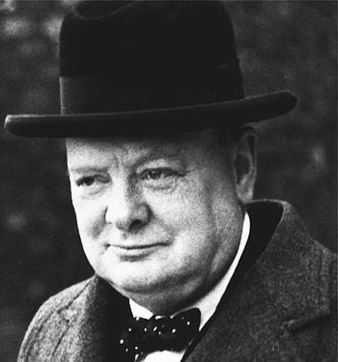
\includegraphics[width=0.6\textwidth]{churchill_winston.jpg}\end{figure}
{\em On May 10, 1940, the Germans began their invasion of France. On June 14 Paris fell. In a matter of days, France would surrender and England would stand as Europe's lone bulwark against the twin evils of Fascism and Nazism. At this critical moment, Churchill gave his third and final speech during the Battle of France, once again imparting words meant to bring hope in this dark hour.}

\vspace{10 mm}

I spoke the other day of the colossal military disaster which occurred when the French High Command failed to withdraw the northern Armies from Belgium at the moment when they knew that the French front was decisively broken at Sedan and on the Meuse. This delay entailed the loss of fifteen or sixteen French divisions and threw out of action for the critical period the whole of the British Expeditionary Force. Our Army and 120,000 French troops were indeed rescued by the British Navy from Dunkirk but only with the loss of their cannon, vehicles and modern equipment. This loss inevitably took some weeks to repair, and in the first two of those weeks the battle in France has been lost. When we consider the heroic resistance made by the French Army against heavy odds in this battle, the enormous losses inflicted upon the enemy and the evident exhaustion of the enemy, it may well be the thought that these 25 divisions of the best-trained and best-equipped troops might have turned the scale. However, General Weygand had to fight without them. Only three British divisions or their equivalent were able to stand in the line with their French comrades. They have suffered severely, but they have fought well. We sent every man we could to France as fast as we could re-equip and transport their formations.

I am not reciting these facts for the purpose of recrimination. That I judge to be utterly futile and even harmful. We cannot afford it. I recite them in order to explain why it was we did not have, as we could have had, between twelve and fourteen British divisions fighting in the line in this great battle instead of only three. Now I put all this aside. I put it on the shelf, from which the historians, when they have time, will select their documents to tell their stories. We have to think of the future and not of the past. This also applies in a small way to our own affairs at home. There are many who would hold an inquest in the House of Commons on the conduct of the Governments-and of Parliaments, for they are in it, too-during the years which led up to this catastrophe. They seek to indict those who were responsible for the guidance of our affairs. This also would be a foolish and pernicious process. There are too many in it. Let each man search his conscience and search his speeches. I frequently search mine.

Of this I am quite sure, that if we open a quarrel between the past and the present, we shall find that we have lost the future. Therefore, I cannot accept the drawing of any distinctions between Members of the present Government. It was formed at a moment of crisis in order to unite all the Parties and all sections of opinion. It has received the almost unanimous support of both Houses of Parliament. Its Members are going to stand together, and, subject to the authority of the House of Commons, we are going to govern the country and fight the war. It is absolutely necessary at a time like this that every Minister who tries each day to do his duty shall be respected; and their subordinates must know that their chiefs are not threatened men, men who are here today and gone tomorrow, but that their directions must be punctually and faithfully obeyed. Without this concentrated power we cannot face what lies before us. I should not think it would be very advantageous for the House to prolong this Debate this afternoon under conditions of public stress. Many facts are not clear that will be clear in a short time. We are to have a secret Session on Thursday, and I should think that would be a better opportunity for the many earnest expressions of opinion which Members will desire to make and for the House to discuss vital matters without having everything read the next morning by our dangerous foes.

The disastrous military events which have happened during the past fortnight have not come to me with any sense of surprise. Indeed, I indicated a fortnight ago as clearly as I could to the House that the worst possibilities were open; and I made it perfectly clear then that whatever happened in France would make no difference to the resolve of Britain and the British Empire to fight on, ‘if necessary for years, if necessary alone.” During the last few days we have successfully brought off the great majority of the troops we had on the line of communication in France; and seven-eighths of the troops we have sent to France since the beginning of the war-that is to say, about 350,000 out of 400,000 men-are safely back in this country. Others are still fighting with the French, and fighting with considerable success in their local encounters against the enemy. We have also brought back a great mass of stores, rifles and munitions of all kinds which had been accumulated in France during the last nine months.

We have, therefore, in this Island today a very large and powerful military force. This force comprises all our best-trained and our finest troops, including scores of thousands of those who have already measured their quality against the Germans and found themselves at no disadvantage. We have under arms at the present time in this Island over a million and a quarter men. Behind these we have the Local Defense Volunteers, numbering half a million, only a portion of whom, however, are yet armed with rifles or other firearms. We have incorporated into our Defense Forces every man for whom we have a weapon. We expect very large additions to our weapons in the near future, and in preparation for this we intend forthwith to call up, drill and train further large numbers. Those who are not called up, or else are employed during the vast business of munitions production in all its branches-and their ramifications are innumerable-will serve their country best by remaining at their ordinary work until they receive their summons. We have also over here Dominions armies. The Canadians had actually landed in France, but have now been safely withdrawn, much disappointed, but in perfect order, with all their artillery and equipment. And these very high-class forces from the Dominions will now take part in the defense of the Mother Country.

Lest the account which I have given of these large forces should raise the question: Why did they not take part in the great battle in France? I must make it clear that, apart from the divisions training and organizing at home, only 12 divisions were equipped to fight upon a scale which justified their being sent abroad. And this was fully up to the number which the French had been led to expect would be available in France at the ninth month of the war. The rest of our forces at home have a fighting value for home defense which will, of course, steadily increase every week that passes. Thus, the invasion of Great Britain would at this time require the transportation across the sea of hostile armies on a very large scale, and after they had been so transported they would have to be continually maintained with all the masses of munitions and supplies which are required for continuous battle-as continuous battle it will surely be.

Here is where we come to the Navy-and after all, we have a Navy. Some people seem to forget that we have a Navy. We must remind them. For the last thirty years I have been concerned in discussions about the possibilities of oversea invasion, and I took the responsibility on behalf of the Admiralty, at the beginning of the last war, of allowing all regular troops to be sent out of the country. That was a very serious step to take, because our Territorials had only just been called up and were quite untrained. Therefore, this Island was for several months particularly denuded of fighting troops. The Admiralty had confidence at that time in their ability to prevent a mass invasion even though at that time the Germans had a magnificent battle fleet in the proportion of 10 to 16, even though they were capable of fighting a general engagement every day and any day, whereas now they have only a couple of heavy ships worth speaking of-the Scharnhorst and the Gneisenau. We are also told that the Italian Navy is to come out and gain sea superiority in these waters. If they seriously intend it, I shall only say that we shall be delighted to offer Signor Mussolini a free and safeguarded passage through the Strait of Gibraltar in order that he may play the part to which he aspires. There is a general curiosity in the British Fleet to find out whether the Italians are up to the level they were at in the last war or whether they have fallen off at all.

Therefore, it seems to me that as far as sea-borne invasion on a great scale is concerned, we are far more capable of meeting it today than we were at many periods in the last war and during the early months of this war, before our other troops were trained, and while the B.E.F. had proceeded abroad. Now, the Navy have never pretended to be able to prevent raids by bodies of 5,000 or 10,000 men flung suddenly across and thrown ashore at several points on the coast some dark night or foggy morning. The efficacy of sea power, especially under modern conditions, depends upon the invading force being of large size; It has to be of large size, in view of our military strength, to be of any use. If it is of large size, then the Navy have something they can find and meet and, as it were, bite on. Now, we must remember that even five divisions, however lightly equipped, would require 200 to 250 ships, and with modern air reconnaissance and photography it would not be easy to collect such an armada, marshal it, and conduct it across the sea without any powerful naval forces to escort it; and there would be very great possibilities, to put it mildly, that this armada would be intercepted long before it reached the coast, and all the men drowned in the sea or, at the worst blown to pieces with their equipment while they were trying to land. We also have a great system of minefields, recently strongly reinforced, through which we alone know the channels. If the enemy tries to sweep passages through these minefields, it will be the task of the Navy to destroy the mine-sweepers and any other forces employed to protect them. There should be no difficulty in this, owing to our great superiority at sea.

Those are the regular, well-tested, well-proved arguments on which we have relied during many years in peace and war. But the question is whether there are any new methods by which those solid assurances can be circumvented. Odd as it may seem, some attention has been given to this by the Admiralty, whose prime duty and responsibility is to destroy any large sea-borne expedition before it reaches, or at the moment when it reaches, these shores. It would not be a good thing for me to go into details of this. It might suggest ideas to other people which they have not thought of, and they would not be likely to give us any of their ideas in exchange. All I will say is that untiring vigilance and mind-searching must be devoted to the subject, because the enemy is crafty and cunning and full of novel treacheries and stratagems. The House may be assured that the utmost ingenuity is being displayed and imagination is being evoked from large numbers of competent officers, well-trained in tactics and thoroughly up to date, to measure and counterwork novel possibilities. Untiring vigilance and untiring searching of the mind is being, and must be, devoted to the subject, because, remember, the enemy is crafty and there is no dirty trick he will not do.

Some people will ask why, then, was it that the British Navy was not able to prevent the movement of a large army from Germany into Norway across the Skagerrak? But the conditions in the Channel and in the North Sea are in no way like those which prevail in the Skagerrak. In the Skagerrak, because of the distance, we could give no air support to our surface ships, and consequently, lying as we did close to the enemy's main air power, we were compelled to use only our submarines. We could not enforce the decisive blockade or interruption which is possible from surface vessels. Our submarines took a heavy toll but could not, by themselves, prevent the invasion of Norway. In the Channel and in the North Sea, on the other hand, our superior naval surface forces, aided by our submarines, will operate with close and effective air assistance.

This brings me, naturally, to the great question of invasion from the air, and of the impending struggle between the British and German Air Forces. It seems quite clear that no invasion on a scale beyond the capacity of our land forces to crush speedily is likely to take place from the air until our Air Force has been definitely overpowered. In the meantime, there may be raids by parachute troops and attempted descents of airborne soldiers. We should be able to give those gentry a warm reception both in the air and on the ground, if they reach it in any condition to continue the dispute. But the great question is: Can we break Hitler's air weapon? Now, of course, it is a very great pity that we have not got an Air Force at least equal to that of the most powerful enemy within striking distance of these shores. But we have a very powerful Air Force which has proved itself far superior in quality, both in men and in many types of machine, to what we have met so far in the numerous and fierce air battles which have been fought with the Germans. In France, where we were at a considerable disadvantage and lost many machines on the ground when they were standing round the aerodromes, we were accustomed to inflict in the air losses of as much as two and two-and-a-half to one. In the fighting over Dunkirk, which was a sort of no-man's-land, we undoubtedly beat the German Air Force, and gained the mastery of the local air, inflicting here a loss of three or four to one day after day. Anyone who looks at the photographs which were published a week or so ago of the re-embarkation, showing the masses of troops assembled on the beach and forming an ideal target for hours at a time, must realize that this re-embarkation would not have been possible unless the enemy had resigned all hope of recovering air superiority at that time and at that place.

In the defense of this Island the advantages to the defenders will be much greater than they were in the fighting around Dunkirk. We hope to improve on the rate of three or four to one which was realized at Dunkirk; and in addition all our injured machines and their crews which get down safely-and, surprisingly, a very great many injured machines and men do get down safely in modern air fighting-all of these will fall, in an attack upon these Islands, on friendly. soil and live to fight another day; whereas all the injured enemy machines and their complements will be total losses as far as the war is concerned.

During the great battle in France, we gave very powerful and continuous aid to. the French Army, both by fighters and bombers; but in spite of every kind of pressure we never would allow the entire metropolitan fighter strength of the Air Force to be consumed. This decision was painful, but it was also right, because the fortunes of the battle in France could not have been decisively affected even if we had thrown in our entire fighter force. That battle was lost by the unfortunate strategical opening, by the extraordinary and unforseen power of the armored columns, and by the great preponderance of the German Army in numbers. Our fighter Air Force might easily have been exhausted as a mere accident in that great struggle, and then we should have found ourselves at the present time in a very serious plight. But as it is, I am happy to inform the House that our fighter strength is stronger at the present time relatively to the Germans, who have suffered terrible losses, than it has ever been; and consequently we believe ourselves possessed of the capacity to continue the war in the air under better conditions than we have ever experienced before. I look forward confidently to the exploits of our fighter pilots-these splendid men, this brilliant youth-who will have the glory of saving their native land, their island home, and all they love, from the most deadly of all attacks.

There remains, of course, the danger of bombing attacks, which will certainly be made very soon upon us by the bomber forces of the enemy. It is true that the German bomber force is superior in numbers to ours; but we have a very large bomber force also, which we shall use to strike at military targets in Germany without intermission. I do not at all underrate the severity of the ordeal which lies before us; but I believe our countrymen will show themselves capable of standing up to it, like the brave men of Barcelona, and will be able to stand up to it, and carry on in spite of it, at least as well as any other people in the world. Much will depend upon this; every man and every woman will have the chance to show the finest qualities of their race, and render the highest service to their cause. For all of us, at this time, whatever our sphere, our station, our occupation or our duties, it will be a help to remember the famous lines: He nothing common did or mean, Upon that memorable scene.

I have thought it right upon this occasion to give the House and the country some indication of the solid, practical grounds upon which we base our inflexible resolve to continue the war. There are a good many people who say, “Never mind. Win or lose, sink or swim, better die than submit to tyranny-and such a tyranny.” And I do not dissociate myself from them. But I can assure them that our professional advisers of the three Services unitedly advise that we should carry on the war, and that there are good and reasonable hopes of final victory. We have fully informed and consulted all the self-governing Dominions, these great communities far beyond the oceans who have been built up on our laws and on our civilization, and who are absolutely free to choose their course, but are absolutely devoted to the ancient Motherland, and who feel themselves inspired by the same emotions which lead me to stake our all upon duty and honor. We have fully consulted them, and I have received from their Prime Ministers, Mr. Mackenzie King of Canada, Mr. Menzies of Australia, Mr. Fraser of New Zealand, and General Smuts of South Africa-that wonderful man, with his immense profound mind, and his eye watching from a distance the whole panorama of European affairs-I have received from all these eminent men, who all have Governments behind them elected on wide franchises, who are all there because they represent the will of their people, messages couched in the most moving terms in which they endorse our decision to fight on, and declare themselves ready to share our fortunes and to persevere to the end. That is what we are going to do.

We may now ask ourselves: In what way has our position worsened since the beginning of the war? It has worsened by the fact that the Germans have conquered a large part of the coast line of Western Europe, and many small countries have been overrun by them. This aggravates the possibilities of air attack and adds to our naval preoccupations. It in no way diminishes, but on the contrary definitely increases, the power of our long-distance blockade. Similarly, the entrance of Italy into the war increases the power of our long-distance blockade. We have stopped the worst leak by that. We do not know whether military resistance will come to an end in France or not, but should it do so, then of course the Germans will be able to concentrate their forces, both military and industrial, upon us. But for the reasons I have given to the House these will not be found so easy to apply. If invasion has become more imminent, as no doubt it has, we, being relieved from the task of maintaining a large army in France, have far larger and more efficient forces to meet it.

If Hitler can bring under his despotic control the industries of the countries he has conquered, this will add greatly to his already vast armament output. On the other hand, this will not happen immediately, and we are now assured of immense, continuous and increasing support in supplies and munitions of all kinds from the United States; and especially of aeroplanes and pilots from the Dominions and across the oceans coming from regions which are beyond the reach of enemy bombers.

I do not see how any of these factors can operate to our detriment on balance before the winter comes; and the winter will impose a strain upon the Nazi regime, with almost all Europe writhing and starving under its cruel heel, which, for all their ruthlessness, will run them very hard. We must not forget that from the moment when we declared war on the 3rd September it was always possible for Germany to turn all her Air Force upon this country, together with any other devices of invasion she might conceive, and that France could have done little or nothing to prevent her doing so. We have, therefore, lived under this danger, in principle and in a slightly modified form, during all these m6nths. In the meanwhile, however, we have enormously improved our methods of defense, and we have learned what we had no right to assume at the beginning, namely, that the individual aircraft and the individual British pilot have a sure and definite superiority. Therefore, in casting up this dread balancesheet and contemplating our dangers with a disillusioned eye, I see great reason for intense vigilance and exertion, but none whatever for panic or despair.

During the first four years of the last war the Allies experienced nothing but disaster and disappointment. That was our constant fear: one blow after another, terrible losses, frightful dangers. Everything miscarried. And yet at the end of those four years the morale of the Allies was higher than that of the Germans, who had moved from one aggressive triumph to another, and who stood everywhere triumphant invaders of the lands into which they had broken. During that war we repeatedly asked ourselves the question: How are we going to win? and no one was able ever to answer it with much precision, until at the end, quite suddenly, quite unexpectedly, our terrible foe collapsed before us, and we were so glutted with victory that in our folly we threw it away.

We do not yet know what will happen in France or whether the French resistance will be prolonged, both in France and in the French Empire overseas. The French Government will be throwing away great opportunities and casting adrift their future if they do not continue the war in accordance with their Treaty obligations, from which we have not felt able to release them. The House will have read the historic declaration in which, at the desire of many Frenchmen-and of our own hearts-we have proclaimed our willingness at the darkest hour in French history to conclude a union of common citizenship in this struggle. However matters may go in France or with the French Government, or other French Governments, we in this Island and in the British Empire will never lose our sense of comradeship with the French people. If we are now called upon to endure what they have been suffering, we shall emulate their courage, and if final victory rewards our toils they shall share the gains, aye, and freedom shall be restored to all. We abate nothing of our just demands; not one jot or tittle do we recede. Czechs, Poles, Norwegians, Dutch, Belgians have joined their causes to our own. All these shall be restored.

What General Weygand called the Battle of France is over. I expect that the Battle of Britain is about to begin. Upon this battle depends the survival of Christian civilization. Upon it depends our own British life, and the long continuity of our institutions and our Empire. The whole fury and might of the enemy must very soon be turned on us. Hitler knows that he will have to break us in this Island or lose the war. If we can stand up to him, all Europe may be free and the life of the world may move forward into broad, sunlit uplands. But if we fail, then the whole world, including the United States, including all that we have known and cared for, will sink into the abyss of a new Dark Age made more sinister, and perhaps more protracted, by the lights of perverted science. Let us therefore brace ourselves to our duties, and so bear ourselves that, if the British Empire and its Commonwealth last for a thousand years, men will still say, “This was their finest hour.”


\chapter{Charles de Gaulle - The Appeal of 18 June}

\textbf{\Large{London -- June 18, 1940 }}

\vspace{10 mm}

\begin{figure}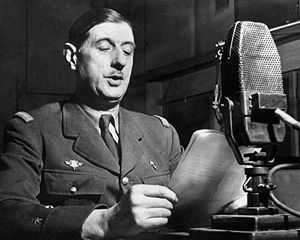
\includegraphics[width=0.6\textwidth]{300px-de-gaulle-radio.jpg}\end{figure}
{\em In June of 1940, it was clear that France was losing their country to the German invasion. Refusing to sign an armistice, Prime Minister Paul Reynaud was forced to resign. He was succeeded by Marshal Philippe Petain who made clear his intention to seek an accommodation with Germany. Disgusted with this decision, General Charles de Gaulle, leader of the Free French Forces, escaped to England on June 15. De Gaulle asked for, and obtained permission from Winston Churchill to make a speech on BBC radio. De Gaulle exhorted the French to not give up hope and to continue the fight against the German occupation and the Vichy Regime.}

\vspace{10 mm}

The leaders who, for many years, were at the head of French armies, have formed a government. This government, alleging our armies to be undone, agreed with the enemy to stop fighting. Of course, we were subdued by the mechanical, ground and air forces of the enemy. Infinitely more than their number, it was the tanks, the airplanes, the tactics of the Germans which made us retreat. It was the tanks, the airplanes, the tactics of the Germans that surprised our leaders to the point to bring them there where they are today.

“But has the last word been said? Must hope disappear? Is defeat final? No!

“Believe me, I speak to you with full knowledge of the facts and tell you that nothing is lost for France. The same means that overcame us can bring us to a day of victory. For France is not alone! She is not alone! She is not alone! She has a vast Empire behind her. She can align with the British Empire that holds the sea and continues the fight. She can, like England, use without limit the immense industry of United States.

“This war is not limited to the unfortunate territory of our country. This war is not finished by the battle of France. This war is a world-wide war. All the faults, all the delays, all the suffering, do not prevent there to be, in the world, all the necessary means to one day crush our enemies. Vanquished today by mechanical force, we will be able to overcome in the future by a superior mechanical force.

“The destiny of the world is here. I, General de Gaulle, currently in London, invite the officers and the French soldiers who are located in British territory or who would come there, with their weapons or without their weapons, I invite the engineers and the special workers of armament industries who are located in British territory or who would come there, to put themselves in contact with me.

“Whatever happens, the flame of the French resistance not must not be extinguished and will not be extinguished. Tomorrow, as today, I will speak on Radio London.”


\chapter{Franklin Delano Roosevelt - Pearl Harbor Address to the Nation}

\textbf{\Large{Washington, D.C. -- December 08, 1941 }}

\vspace{10 mm}

\begin{figure}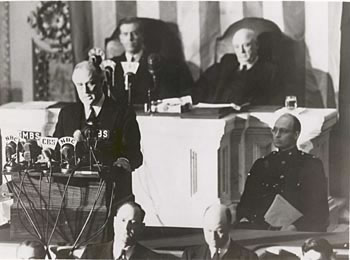
\includegraphics[width=0.6\textwidth]{fdr-day-of-infamy-speech.jpg}\end{figure}
{\em The attack on Pearl Harbor, December 7, 1941, shocked the United States to its core, outraging a nation that had hoped to stay out of the mounting turmoil in Asia and Europe. Overnight, the country united in desire to enter the war. The day after the attacks, FDR addressed the nation in a brief, but electrifying speech, declaring war on Japan and giving assurance that the United States would attain victory.

Be sure to listen to the audio of the speech. Imagine every American family, rattled and worried, listening around the radio to what their president would say. They knew their whole world was about to change forever. Listen to the reaction of Congress as they applaud and cheer FDR's words. The emotion is so very real and palatable; it truly transports you back to that critical moment in time.}

\vspace{10 mm}

Mr. Vice President, Mr. Speaker, Members of the Senate, and of the House of Representatives:

Yesterday, December 7th, 1941 — a date which will live in infamy — the United States of America was suddenly and deliberately attacked by naval and air forces of the Empire of Japan.

The United States was at peace with that nation and, at the solicitation of Japan, was still in conversation with its government and its emperor looking toward the maintenance of peace in the Pacific.

Indeed, one hour after Japanese air squadrons had commenced bombing in the American island of Oahu, the Japanese ambassador to the United States and his colleague delivered to our Secretary of State a formal reply to a recent American message. And while this reply stated that it seemed useless to continue the existing diplomatic negotiations, it contained no threat or hint of war or of armed attack.

It will be recorded that the distance of Hawaii from Japan makes it obvious that the attack was deliberately planned many days or even weeks ago. During the intervening time, the Japanese government has deliberately sought to deceive the United States by false statements and expressions of hope for continued peace.

The attack yesterday on the Hawaiian islands has caused severe damage to American naval and military forces. I regret to tell you that very many American lives have been lost. In addition, American ships have been reported torpedoed on the high seas between San Francisco and Honolulu.

Yesterday, the Japanese government also launched an attack against Malaya.

Last night, Japanese forces attacked Hong Kong.

Last night, Japanese forces attacked Guam.

Last night, Japanese forces attacked the Philippine Islands.

Last night, the Japanese attacked Wake Island.

And this morning, the Japanese attacked Midway Island.

Japan has, therefore, undertaken a surprise offensive extending throughout the Pacific area. The facts of yesterday and today speak for themselves. The people of the United States have already formed their opinions and well understand the implications to the very life and safety of our nation.

As commander in chief of the Army and Navy, I have directed that all measures be taken for our defense. But always will our whole nation remember the character of the onslaught against us.

No matter how long it may take us to overcome this premeditated invasion, the American people in their righteous might will win through to absolute victory.

I believe that I interpret the will of the Congress and of the people when I assert that we will not only defend ourselves to the uttermost, but will make it very certain that this form of treachery shall never again endanger us.

Hostilities exist. There is no blinking at the fact that our people, our territory, and our interests are in grave danger.

With confidence in our armed forces, with the unbounding determination of our people, we will gain the inevitable triumph — so help us God.

I ask that the Congress declare that since the unprovoked and dastardly attack by Japan on Sunday, December 7th, 1941, a state of war has existed between the United States and the Japanese empire.


\chapter{Mahatma Gandhi - Quit India}

\textbf{\Large{India -- August 08, 1942 }}

\vspace{10 mm}

\begin{figure}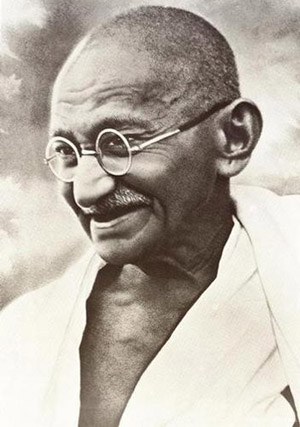
\includegraphics[width=0.6\textwidth]{gandhi.jpg}\end{figure}
{\em While the battle for freedom and democracy raged across the world, the people of India were engaged in their own fight for liberty. For almost a century, India had been under the direct rule of the British crown, and many Indians had had enough. Mahatma Gandhi and the National Indian Congress pushed for a completely non-violent movement aimed at forcing Britain to “Quit India.” Gandhi, pioneer of the tactics of non-violent civil disobedience, called for their use on August 8, 1942 with the passing of the Quit India Resolution demanding complete independence from British rule.}

\vspace{10 mm}

Before you discuss the resolution, let me place before you one or two things, I want you to understand two things very clearly and to consider them from the same point of view from which I am placing them before you. I ask you to consider it from my point of view, because if you approve of it, you will be enjoined to carry out all I say. It will be a great responsibility. There are people who ask me whether I am the same man that I was in 1920, or whether there has been any change in me. You are right in asking that question.

Let me, however, hasten to assure that I am the same Gandhi as I was in 1920. I have not changed in any fundamental respect. I attach the same importance to non-violence that I did then. If at all, my emphasis on it has grown stronger. There is no real contradiction between the present resolution and my previous writings and utterances.

Occasions like the present do not occur in everybody's and but rarely in anybody's life. I want you to know and feel that there is nothing but purest Ahimsa1 in all that I am saying and doing today. The draft resolution of the Working Committee is based on Ahimsa, the contemplated struggle similarly has its roots in Ahimsa. If, therefore, there is any among you who has lost faith in Ahimsa or is wearied of it, let him not vote for this resolution.

Let me explain my position clearly. God has vouchsafed to me a priceless gift in the weapon of Ahimsa. I and my Ahimsa are on our trail today. If in the present crisis, when the earth is being scorched by the flames of Himsa2 and crying for deliverance, I failed to make use of the God given talent, God will not forgive me and I shall be judged un-wrongly of the great gift. I must act now. I may not hesitate and merely look on, when Russia and China are threatened.

Ours is not a drive for power, but purely a non-violent fight for India's independence. In a violent struggle, a successful general has been often known to effect a military coup and to set up a dictatorship. But under the Congress scheme of things, essentially non-violent as it is, there can be no room for dictatorship. A non-violent soldier of freedom will covet nothing for himself, he fights only for the freedom of his country. The Congress is unconcerned as to who will rule, when freedom is attained. The power, when it comes, will belong to the people of India, and it will be for them to decide to whom it placed in the entrusted. May be that the reins will be placed in the hands of the Parsis, for instance-as I would love to see happen-or they may be handed to some others whose names are not heard in the Congress today. It will not be for you then to object saying, “This community is microscopic. That party did not play its due part in the freedom's struggle; why should it have all the power?” Ever since its inception the Congress has kept itself meticulously free of the communal taint. It has thought always in terms of the whole nation and has acted accordingly\ldots

I know how imperfect our Ahimsa is and how far away we are still from the ideal, but in Ahimsa there is no final failure or defeat. I have faith, therefore, that if, in spite of our shortcomings, the big thing does happen, it will be because God wanted to help us by crowning with success our silent, unremitting Sadhana1 for the last twenty-two years.

I believe that in the history of the world, there has not been a more genuinely democratic struggle for freedom than ours. I read Carlyle's French Resolution while I was in prison, and Pandit Jawaharlal has told me something about the Russian revolution. But it is my conviction that inasmuch as these struggles were fought with the weapon of violence they failed to realize the democratic ideal. In the democracy which I have envisaged, a democracy established by non-violence, there will be equal freedom for all. Everybody will be his own master. It is to join a struggle for such democracy that I invite you today. Once you realize this you will forget the differences between the Hindus and Muslims, and think of yourselves as Indians only, engaged in the common struggle for independence.

Then, there is the question of your attitude towards the British. I have noticed that there is hatred towards the British among the people. The people say they are disgusted with their behaviour. The people make no distinction between British imperialism and the British people. To them, the two are one This hatred would even make them welcome the Japanese. It is most dangerous. It means that they will exchange one slavery for another. We must get rid of this feeling. Our quarrel is not with the British people, we fight their imperialism. The proposal for the withdrawal of British power did not come out of anger. It came to enable India to play its due part at the present critical juncture It is not a happy position for a big country like India to be merely helping with money and material obtained willy-nilly from her while the United Nations are conducting the war. We cannot evoke the true spirit of sacrifice and velour, so long as we are not free. I know the British Government will not be able to withhold freedom from us, when we have made enough self-sacrifice. We must, therefore, purge ourselves of hatred. Speaking for myself, I can say that I have never felt any hatred. As a matter of fact, I feel myself to be a greater friend of the British now than ever before. One reason is that they are today in distress. My very friendship, therefore, demands that I should try to save them from their mistakes. As I view the situation, they are on the brink of an abyss. It, therefore, becomes my duty to warn them of their danger even though it may, for the time being, anger them to the point of cutting off the friendly hand that is stretched out to help them. People may laugh, nevertheless that is my claim. At a time when I may have to launch the biggest struggle of my life, I may not harbour hatred against anybody.


\chapter{William Faulkner - Nobel Prize Acceptance Speech}

\textbf{\Large{Stockholm, Sweden -- December 10, 1950 }}

\vspace{10 mm}

\begin{figure}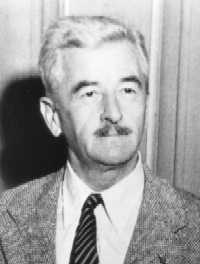
\includegraphics[width=0.6\textwidth]{williamfaulkner.jpg}\end{figure}
{\em A true master of the written word, William Faulkner did not often make public his gift for the spoken variety. So there was some interest as to what he would say when accepting the Nobel Peace Prize for his “powerful and artistically unique contribution to the modern American novel.” The year was 1950, the Soviet Union had tapped the potential of the atomic bomb, and the atmosphere in the the United States crackled with the fear of them using it. Faulkner challenged poets, authors, and all mankind to think beyond the questions of “When will I be blown up?” and instead continue to “create out of the materials of the human spirit something which did not exist before.”}

\vspace{10 mm}

I feel that this award was not made to me as a man, but to my work--a life's work in the agony and sweat of the human spirit, not for glory and least of all for profit, but to create out of the materials of the human spirit something which did not exist before. So this award is only mine in trust. It will not be difficult to find a dedication for the money part of it commensurate with the purpose and significance of its origin. But I would like to do the same with the acclaim too, by using this moment as a pinnacle from which I might be listened to by the young men and women already dedicated to the same anguish and travail, among whom is already that one who will some day stand where I am standing.

Our tragedy today is a general and universal physical fear so long sustained by now that we can even bear it. There are no longer problems of the spirit. There is only one question: When will I be blown up? Because of this, the young man or woman writing today has forgotten the problems of the human heart in conflict with itself which alone can make good writing because only that is worth writing about, worth the agony and the sweat. He must learn them again. He must teach himself that the basest of all things is to be afraid: and, teaching himself that, forget it forever, leaving no room in his workshop for anything but the old verities and truths of the heart, the universal truths lacking which any story is ephemeral and doomed--love and honor and pity and pride and compassion and sacrifice. Until he does so, he labors under a curse. He writes not of love but of lust, of defeats in which nobody loses anything of value, and victories without hope and worst of all, without pity or compassion. His griefs grieve on no universal bones, leaving no scars. He writes not of the heart but of the glands.

Until he learns these things, he will write as though he stood among and watched the end of man. I decline to accept the end of man. It is easy enough to say that man is immortal because he will endure: that when the last ding-dong of doom has clanged and faded from the last worthless rock hanging tideless in the last red and dying evening, that even then there will still be one more sound: that of his puny inexhaustible voice, still talking. I refuse to accept this. I believe that man will not merely endure: he will prevail. He is immortal, not because he alone among creatures has an inexhaustible voice, but because he has a soul, a spirit capable of compassion and sacrifice and endurance. The poet's, the writer's, duty is to write about these things. It is his privilege to help man endure by lifting his heart, by reminding him of the courage and honor and hope and pride and compassion and pity and sacrifice which have been the glory of his past. The poet's voice need not merely be the record of man, it can be one of the props, the pillars to help him endure and prevail.


\chapter{General Douglas MacArthur - Farewell Address to Congress}

\textbf{\Large{Washington D.C. -- April 19, 1951 }}

\vspace{10 mm}

\begin{figure}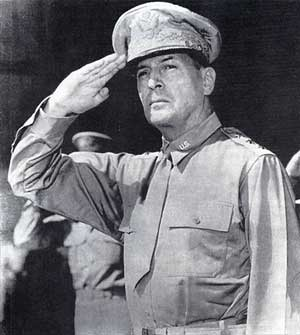
\includegraphics[width=0.6\textwidth]{douglasmacarthursalute.jpg}\end{figure}
{\em During the Korean War, General MacArthur and President Truman clashed over the threat posed by the Chinese People's Liberation Army and their incursion into Korea. MacArthur continually pressed Truman for permission to bomb bases in Manchuria, believing the war needed to be extended in area and scope. Truman refused the General's requests, arguing that directly drawing China into the war would arouse the Soviet Union to action. MacArthur continued to press his case, and Truman, accusing the General of insubordination, made the decision to relieve MacArthur of his command. After serving for 52 years and in three wars, the General's military career was over. MacArthur returned to the United States and gave this farewell address to Congress.}

\vspace{10 mm}

Mr. President, Mr. Speaker, and Distinguished Members of the Congress:

I stand on this rostrum with a sense of deep humility and great pride — humility in the wake of those great American architects of our history who have stood here before me; pride in the reflection that this forum of legislative debate represents human liberty in the purest form yet devised. Here are centered the hopes and aspirations and faith of the entire human race. I do not stand here as advocate for any partisan cause, for the issues are fundamental and reach quite beyond the realm of partisan consideration. They must be resolved on the highest plane of national interest if our course is to prove sound and our future protected. I trust, therefore, that you will do me the justice of receiving that which I have to say as solely expressing the considered viewpoint of a fellow American.

I address you with neither rancor nor bitterness in the fading twilight of life, with but one purpose in mind: to serve my country. The issues are global and so interlocked that to consider the problems of one sector, oblivious to those of another, is but to court disaster for the whole. While Asia is commonly referred to as the Gateway to Europe, it is no less true that Europe is the Gateway to Asia, and the broad influence of the one cannot fail to have its impact upon the other. There are those who claim our strength is inadequate to protect on both fronts, that we cannot divide our effort. I can think of no greater expression of defeatism. If a potential enemy can divide his strength on two fronts, it is for us to counter his effort. The Communist threat is a global one. Its successful advance in one sector threatens the destruction of every other sector. You can not appease or otherwise surrender to communism in Asia without simultaneously undermining our efforts to halt its advance in Europe.

Beyond pointing out these general truisms, I shall confine my discussion to the general areas of Asia. Before one may objectively assess the situation now existing there, he must comprehend something of Asia's past and the revolutionary changes which have marked her course up to the present. Long exploited by the so-called colonial powers, with little opportunity to achieve any degree of social justice, individual dignity, or a higher standard of life such as guided our own noble administration in the Philippines, the peoples of Asia found their opportunity in the war just past to throw off the shackles of colonialism and now see the dawn of new opportunity, a heretofore unfelt dignity, and the self-respect of political freedom.

Mustering half of the earth's population, and 60 percent of its natural resources these peoples are rapidly consolidating a new force, both moral and material, with which to raise the living standard and erect adaptations of the design of modern progress to their own distinct cultural environments. Whether one adheres to the concept of colonization or not, this is the direction of Asian progress and it may not be stopped. It is a corollary to the shift of the world economic frontiers as the whole epicenter of world affairs rotates back toward the area whence it started.

In this situation, it becomes vital that our own country orient its policies in consonance with this basic evolutionary condition rather than pursue a course blind to the reality that the colonial era is now past and the Asian peoples covet the right to shape their own free destiny. What they seek now is friendly guidance, understanding, and support — not imperious direction — the dignity of equality and not the shame of subjugation. Their pre-war standard of life, pitifully low, is infinitely lower now in the devastation left in war's wake. World ideologies play little part in Asian thinking and are little understood. What the peoples strive for is the opportunity for a little more food in their stomachs, a little better clothing on their backs, a little firmer roof over their heads, and the realization of the normal nationalist urge for political freedom. These political-social conditions have but an indirect bearing upon our own national security, but do form a backdrop to contemporary planning which must be thoughtfully considered if we are to avoid the pitfalls of unrealism.

Of more direct and immediately bearing upon our national security are the changes wrought in the strategic potential of the Pacific Ocean in the course of the past war. Prior thereto the western strategic frontier of the United States lay on the littoral line of the Americas, with an exposed island salient extending out through Hawaii, Midway, and Guam to the Philippines. That salient proved not an outpost of strength but an avenue of weakness along which the enemy could and did attack.

The Pacific was a potential area of advance for any predatory force intent upon striking at the bordering land areas. All this was changed by our Pacific victory. Our strategic frontier then shifted to embrace the entire Pacific Ocean, which became a vast moat to protect us as long as we held it. Indeed, it acts as a protective shield for all of the Americas and all free lands of the Pacific Ocean area. We control it to the shores of Asia by a chain of islands extending in an arc from the Aleutians to the Mariannas held by us and our free allies. From this island chain we can dominate with sea and air power every Asiatic port from Vladivostok to Singapore — with sea and air power every port, as I said, from Vladivostok to Singapore — and prevent any hostile movement into the Pacific.

*Any predatory attack from Asia must be an amphibious effort.* No amphibious force can be successful without control of the sea lanes and the air over those lanes in its avenue of advance. With naval and air supremacy and modest ground elements to defend bases, any major attack from continental Asia toward us or our friends in the Pacific would be doomed to failure.

Under such conditions, the Pacific no longer represents menacing avenues of approach for a prospective invader. It assumes, instead, the friendly aspect of a peaceful lake. Our line of defense is a natural one and can be maintained with a minimum of military effort and expense. It envisions no attack against anyone, nor does it provide the bastions essential for offensive operations, but properly maintained, would be an invincible defense against aggression. The holding of this littoral defense line in the western Pacific is entirely dependent upon holding all segments thereof; for any major breach of that line by an unfriendly power would render vulnerable to determined attack every other major segment.

This is a military estimate as to which I have yet to find a military leader who will take exception. For that reason, I have strongly recommended in the past, as a matter of military urgency, that under no circumstances must Formosa fall under Communist control. Such an eventuality would at once threaten the freedom of the Philippines and the loss of Japan and might well force our western frontier back to the coast of California, Oregon and Washington.

To understand the changes which now appear upon the Chinese mainland, one must understand the changes in Chinese character and culture over the past 50 years. China, up to 50 years ago, was completely non-homogenous, being compartmented into groups divided against each other. The war-making tendency was almost non-existent, as they still followed the tenets of the Confucian ideal of pacifist culture. At the turn of the century, under the regime of Chang Tso Lin, efforts toward greater homogeneity produced the start of a nationalist urge. This was further and more successfully developed under the leadership of Chiang Kai-Shek, but has been brought to its greatest fruition under the present regime to the point that it has now taken on the character of a united nationalism of increasingly dominant, aggressive tendencies.

Through these past 50 years the Chinese people have thus become militarized in their concepts and in their ideals. They now constitute excellent soldiers, with competent staffs and commanders. This has produced a new and dominant power in Asia, which, for its own purposes, is allied with Soviet Russia but which in its own concepts and methods has become aggressively imperialistic, with a lust for expansion and increased power normal to this type of imperialism.

There is little of the ideological concept either one way or another in the Chinese make-up. The standard of living is so low and the capital accumulation has been so thoroughly dissipated by war that the masses are desperate and eager to follow any leadership which seems to promise the alleviation of local stringencies.

I have from the beginning believed that the Chinese Communists' support of the North Koreans was the dominant one. Their interests are, at present, parallel with those of the Soviet. But I believe that the aggressiveness recently displayed not only in Korea but also in Indo-China and Tibet and pointing potentially toward the South reflects predominantly the same lust for the expansion of power which has animated every would-be conqueror since the beginning of time.

The Japanese people, since the war, have undergone the greatest reformation recorded in modern history. With a commendable will, eagerness to learn, and marked capacity to understand, they have, from the ashes left in war's wake, erected in Japan an edifice dedicated to the supremacy of individual liberty and personal dignity; and in the ensuing process there has been created a truly representative government committed to the advance of political morality, freedom of economic enterprise, and social justice.

Politically, economically, and socially Japan is now abreast of many free nations of the earth and will not again fail the universal trust. That it may be counted upon to wield a profoundly beneficial influence over the course of events in Asia is attested by the magnificent manner in which the Japanese people have met the recent challenge of war, unrest, and confusion surrounding them from the outside and checked communism within their own frontiers without the slightest slackening in their forward progress. I sent all four of our occupation divisions to the Korean battlefront without the slightest qualms as to the effect of the resulting power vacuum upon Japan. The results fully justified my faith. I know of no nation more serene, orderly, and industrious, nor in which higher hopes can be entertained for future constructive service in the advance of the human race.

Of our former ward, the Philippines, we can look forward in confidence that the existing unrest will be corrected and a strong and healthy nation will grow in the longer aftermath of war's terrible destructiveness. We must be patient and understanding and never fail them — as in our hour of need, they did not fail us. A Christian nation, the Philippines stand as a mighty bulwark of Christianity in the Far East, and its capacity for high moral leadership in Asia is unlimited.

On Formosa, the government of the Republic of China has had the opportunity to refute by action much of the malicious gossip which so undermined the strength of its leadership on the Chinese mainland. The Formosan people are receiving a just and enlightened administration with majority representation on the organs of government, and politically, economically, and socially they appear to be advancing along sound and constructive lines.

With this brief insight into the surrounding areas, I now turn to the Korean conflict. While I was not consulted prior to the President's decision to intervene in support of the Republic of Korea, that decision from a military standpoint, proved a sound one, as we hurled back the invader and decimated his forces. Our victory was complete, and our objectives within reach, when Red China intervened with numerically superior ground forces.

This created a new war and an entirely new situation, a situation not contemplated when our forces were committed against the North Korean invaders; a situation which called for new decisions in the diplomatic sphere to permit the realistic adjustment of military strategy.

Such decisions have not been forthcoming.

While no man in his right mind would advocate sending our ground forces into continental China, and such was never given a thought, the new situation did urgently demand a drastic revision of strategic planning if our political aim was to defeat this new enemy as we had defeated the old.

Apart from the military need, as I saw It, to neutralize the sanctuary protection given the enemy north of the Yalu, I felt that military necessity in the conduct of the war made necessary: first the intensification of our economic blockade against China; two the imposition of a naval blockade against the China coast; three removal of restrictions on air reconnaissance of China's coastal areas and of Manchuria; four removal of restrictions on the forces of the Republic of China on Formosa, with logistical support to contribute to their effective operations against the common enemy.

For entertaining these views, all professionally designed to support our forces committed to Korea and bring hostilities to an end with the least possible delay and at a saving of countless American and allied lives, I have been severely criticized in lay circles, principally abroad, despite my understanding that from a military standpoint the above views have been fully shared in the past by practically every military leader concerned with the Korean campaign, including our own Joint Chiefs of Staff.

I called for reinforcements but was informed that reinforcements were not available. I made clear that if not permitted to destroy the enemy built-up bases north of the Yalu, if not permitted to utilize the friendly Chinese Force of some 600,000 men on Formosa, if not permitted to blockade the China coast to prevent the Chinese Reds from getting succor from without, and if there were to be no hope of major reinforcements, the position of the command from the military standpoint forbade victory.

We could hold in Korea by constant maneuver and in an approximate area where our supply line advantages were in balance with the supply line disadvantages of the enemy, but we could hope at best for only an indecisive campaign with its terrible and constant attrition upon our forces if the enemy utilized its full military potential. I have constantly called for the new political decisions essential to a solution.

Efforts have been made to distort my position. It has been said, in effect, that I was a warmonger. Nothing could be further from the truth. I know war as few other men now living know it, and nothing to me is more revolting. I have long advocated its complete abolition, as its very destructiveness on both friend and foe has rendered it useless as a means of settling international disputes. Indeed, on the second day of September, nineteen hundred and forty-five, just following the surrender of the Japanese nation on the Battleship Missouri, I formally cautioned as follows:

\begin{quote}Men since the beginning of time have sought peace. Various methods through the ages have been attempted to devise an international process to prevent or settle disputes between nations. From the very start workable methods were found in so far as individual citizens were concerned, but the mechanics of an instrumentality of larger international scope have never been successful. Military alliances, balances of power, Leagues of Nations, all in turn failed, leaving the only path to be by way of the crucible of war. The utter  destructiveness of war now blocks out this alternative. We have had our last chance. If we will not devise some greater and more equitable system, Armageddon will be at our door. The problem basically is theological and involves a spiritual recrudescence and improvement of human character that will synchronize with our almost matchless advances in science, art, literature, and all material and cultural developments of the past 2000 years. It must be of the spirit if we are to save the flesh.\end{quote}

But once war is forced upon us, there is no other alternative than to apply every available means to bring it to a swift end.

War's very object is victory, not prolonged indecision.

In war there is no substitute for victory.

There are some who, for varying reasons, would appease Red China. They are blind to history's clear lesson, for history teaches with unmistakable emphasis that appeasement but begets new and bloodier war. It points to no single instance where this end has justified that means, where appeasement has led to more than a sham peace. Like blackmail, it lays the basis for new and successively greater demands until, as in blackmail, violence becomes the only other alternative.

“Why,” my soldiers asked of me, “surrender military advantages to an enemy in the field?” I could not answer.

Some may say: to avoid spread of the conflict into an all-out war with China; others, to avoid Soviet intervention. Neither explanation seems valid, for China is already engaging with the maximum power it can commit, and the Soviet will not necessarily mesh its actions with our moves. Like a cobra, any new enemy will more likely strike whenever it feels that the relativity in military or other potential is in its favor on a world-wide basis.

The tragedy of Korea is further heightened by the fact that its military action is confined to its territorial limits. It condemns that nation, which it is our purpose to save, to suffer the devastating impact of full naval and air bombardment while the enemy's sanctuaries are fully protected from such attack and devastation.

Of the nations of the world, Korea alone, up to now, is the sole one which has risked its all against communism. The magnificence of the courage and fortitude of the Korean people defies description.

They have chosen to risk death rather than slavery. Their last words to me were: “Don't scuttle the Pacific!”

I have just left your fighting sons in Korea. They have met all tests there, and I can report to you without reservation that they are splendid in every way.

It was my constant effort to preserve them and end this savage conflict honorably and with the least loss of time and a minimum sacrifice of life. Its growing bloodshed has caused me the deepest anguish and anxiety.

Those gallant men will remain often in my thoughts and in my prayers always.

I am closing my 52 years of military service. When I joined the Army, even before the turn of the century, it was the fulfillment of all of my boyish hopes and dreams. The world has turned over many times since I took the oath on the plain at West Point, and the hopes and dreams have long since vanished, but I still remember the refrain of one of the most popular barrack ballads of that day which proclaimed most proudly that “old soldiers never die; they just fade away.”

And like the old soldier of that ballad, I now close my military career and just fade away, an old soldier who tried to do his duty as God gave him the light to see that duty.

Good Bye.


\chapter{Dwight D. Eisenhower - Farewell Address}

\textbf{\Large{Washington, D.C. -- January 17, 1961 }}

\vspace{10 mm}

\begin{figure}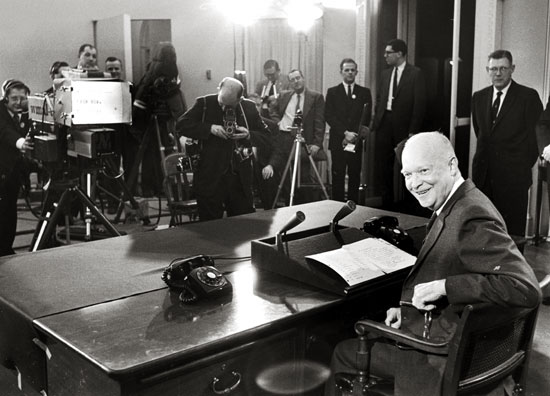
\includegraphics[width=0.6\textwidth]{image.jpeg}\end{figure}
{\em The 1950's were a time of ever increasing military spending, as the United States sought to fight communism abroad and prevent it at home. As President Dwight D. Eisenhower left office, more than half of the federal budget was allocated for defense purposes. Eisenhower, former General of the Army, was certainly not opposed to the use of military power to keep the peace. Still, he saw fit to use his “Farewell Address” to warn the nation of the dangers posed by the “military-industrial complex,” referring to the relationship between the armed forces, the government, and the suppliers of war materials. Eisenhower was wary of the large role defense spending played in the economy, and understood the political and corporate corruption that could result if the public was not vigilant in checking it.}

\vspace{10 mm}

Good evening, my fellow Americans.

First, I should like to express my gratitude to the radio and television networks for the opportunities they have given me over the years to bring reports and messages to our nation. My special thanks go to them for the opportunity of addressing you this evening.

Three days from now, after half century in the service of our country, I shall lay down the responsibilities of office as, in traditional and solemn ceremony, the authority of the Presidency is vested in my successor. This evening, I come to you with a message of leave-taking and farewell, and to share a few final thoughts with you, my countrymen.

Like every other — Like every other citizen, I wish the new President, and all who will labor with him, Godspeed. I pray that the coming years will be blessed with peace and prosperity for all.

Our people expect their President and the Congress to find essential agreement on issues of great moment, the wise resolution of which will better shape the future of the nation. My own relations with the Congress, which began on a remote and tenuous basis when, long ago, a member of the Senate appointed me to West Point, have since ranged to the intimate during the war and immediate post-war period, and finally to the mutually interdependent during these past eight years. In this final relationship, the Congress and the Administration have, on most vital issues, cooperated well, to serve the nation good, rather than mere partisanship, and so have assured that the business of the nation should go forward. So, my official relationship with the Congress ends in a feeling — on my part — of gratitude that we have been able to do so much together.

We now stand ten years past the midpoint of a century that has witnessed four major wars among great nations. Three of these involved our own country. Despite these holocausts, America is today the strongest, the most influential, and most productive nation in the world. Understandably proud of this pre-eminence, we yet realize that America's leadership and prestige depend, not merely upon our unmatched material progress, riches, and military strength, but on how we use our power in the interests of world peace and human betterment.

Throughout America's adventure in free government, our basic purposes have been to keep the peace, to foster progress in human achievement, and to enhance liberty, dignity, and integrity among peoples and among nations. To strive for less would be unworthy of a free and religious people. Any failure traceable to arrogance, or our lack of comprehension, or readiness to sacrifice would inflict upon us grievous hurt, both at home and abroad.

Progress toward these noble goals is persistently threatened by the conflict now engulfing the world. It commands our whole attention, absorbs our very beings. We face a hostile ideology global in scope, atheistic in character, ruthless in purpose, and insiduous [insidious] in method. Unhappily, the danger it poses promises to be of indefinite duration. To meet it successfully, there is called for, not so much the emotional and transitory sacrifices of crisis, but rather those which enable us to carry forward steadily, surely, and without complaint the burdens of a prolonged and complex struggle with liberty the stake. Only thus shall we remain, despite every provocation, on our charted course toward permanent peace and human betterment.

Crises there will continue to be. In meeting them, whether foreign or domestic, great or small, there is a recurring temptation to feel that some spectacular and costly action could become the miraculous solution to all current difficulties. A huge increase in newer elements of our defenses; development of unrealistic programs to cure every ill in agriculture; a dramatic expansion in basic and applied research — these and many other possibilities, each possibly promising in itself, may be suggested as the only way to the road we wish to travel.

But each proposal must be weighed in the light of a broader consideration: the need to maintain balance in and among national programs, balance between the private and the public economy, balance between the cost and hoped for advantages, balance between the clearly necessary and the comfortably desirable, balance between our essential requirements as a nation and the duties imposed by the nation upon the individual, balance between actions of the moment and the national welfare of the future. Good judgment seeks balance and progress. Lack of it eventually finds imbalance and frustration. The record of many decades stands as proof that our people and their Government have, in the main, understood these truths and have responded to them well, in the face of threat and stress.

But threats, new in kind or degree, constantly arise. Of these, I mention two only.

A vital element in keeping the peace is our military establishment. Our arms must be mighty, ready for instant action, so that no potential aggressor may be tempted to risk his own destruction. Our military organization today bears little relation to that known of any of my predecessors in peacetime, or, indeed, by the fighting men of World War II or Korea.

Until the latest of our world conflicts, the United States had no armaments industry. American makers of plowshares could, with time and as required, make swords as well. But we can no longer risk emergency improvisation of national defense. We have been compelled to create a permanent armaments industry of vast proportions. Added to this, three and a half million men and women are directly engaged in the defense establishment. We annually spend on military security alone more than the net income of all United States cooperations — corporations.

Now this conjunction of an immense military establishment and a large arms industry is new in the American experience. The total influence — economic, political, even spiritual — is felt in every city, every Statehouse, every office of the Federal government. We recognize the imperative need for this development. Yet, we must not fail to comprehend its grave implications. Our toil, resources, and livelihood are all involved. So is the very structure of our society.

In the councils of government, we must guard against the acquisition of unwarranted influence, whether sought or unsought, by the military-industrial complex. The potential for the disastrous rise of misplaced power exists and will persist. We must never let the weight of this combination endanger our liberties or democratic processes. We should take nothing for granted. Only an alert and knowledgeable citizenry can compel the proper meshing of the huge industrial and military machinery of defense with our peaceful methods and goals, so that security and liberty may prosper together.

Akin to, and largely responsible for the sweeping changes in our industrial-military posture, has been the technological revolution during recent decades. In this revolution, research has become central; it also becomes more formalized, complex, and costly. A steadily increasing share is conducted for, by, or at the direction of, the Federal government.

Today, the solitary inventor, tinkering in his shop, has been overshadowed by task forces of scientists in laboratories and testing fields. In the same fashion, the free university, historically the fountainhead of free ideas and scientific discovery, has experienced a revolution in the conduct of research. Partly because of the huge costs involved, a government contract becomes virtually a substitute for intellectual curiosity. For every old blackboard there are now hundreds of new electronic computers. The prospect of domination of the nation's scholars by Federal employment, project allocations, and the power of money is ever present — and is gravely to be regarded.

Yet, in holding scientific research and discovery in respect, as we should, we must also be alert to the equal and opposite danger that public policy could itself become the captive of a scientific-technological elite.

It is the task of statesmanship to mold, to balance, and to integrate these and other forces, new and old, within the principles of our democratic system — ever aiming toward the supreme goals of our free society.

Another factor in maintaining balance involves the element of time. As we peer into society's future, we — you and I, and our government — must avoid the impulse to live only for today, plundering for our own ease and convenience the precious resources of tomorrow. We cannot mortgage the material assets of our grandchildren without risking the loss also of their political and spiritual heritage. We want democracy to survive for all generations to come, not to become the insolvent phantom of tomorrow.

During the long lane of the history yet to be written, America knows that this world of ours, ever growing smaller, must avoid becoming a community of dreadful fear and hate, and be, instead, a proud confederation of mutual trust and respect. Such a confederation must be one of equals. The weakest must come to the conference table with the same confidence as do we, protected as we are by our moral, economic, and military strength. That table, though scarred by many fast frustrations — past frustrations, cannot be abandoned for the certain agony of disarmament — of the battlefield.

Disarmament, with mutual honor and confidence, is a continuing imperative. Together we must learn how to compose differences, not with arms, but with intellect and decent purpose. Because this need is so sharp and apparent, I confess that I lay down my official responsibilities in this field with a definite sense of disappointment. As one who has witnessed the horror and the lingering sadness of war, as one who knows that another war could utterly destroy this civilization which has been so slowly and painfully built over thousands of years, I wish I could say tonight that a lasting peace is in sight.

Happily, I can say that war has been avoided. Steady progress toward our ultimate goal has been made. But so much remains to be done. As a private citizen, I shall never cease to do what little I can to help the world advance along that road.

So, in this, my last good night to you as your President, I thank you for the many opportunities you have given me for public service in war and in peace. I trust in that — in that — in that service you find some things worthy. As for the rest of it, I know you will find ways to improve performance in the future.

You and I, my fellow citizens, need to be strong in our faith that all nations, under God, will reach the goal of peace with justice. May we be ever unswerving in devotion to principle, confident but humble with power, diligent in pursuit of the Nations' great goals.

To all the peoples of the world, I once more give expression to America's prayerful and continuing aspiration: We pray that peoples of all faiths, all races, all nations, may have their great human needs satisfied; that those now denied opportunity shall come to enjoy it to the full; that all who yearn for freedom may experience its few spiritual blessings. Those who have freedom will understand, also, its heavy responsibility; that all who are insensitive to the needs of others will learn charity; and that the sources — scourges of poverty, disease, and ignorance will be made [to] disappear from the earth; and that in the goodness of time, all peoples will come to live together in a peace guaranteed by the binding force of mutual respect and love.

Now, on Friday noon, I am to become a private citizen. I am proud to do so. I look forward to it.

Thank you, and good night.


\chapter{John F. Kennedy - Inauguration Address}

\textbf{\Large{Washington D.C. -- January 20, 1961 }}

\vspace{10 mm}

\begin{figure}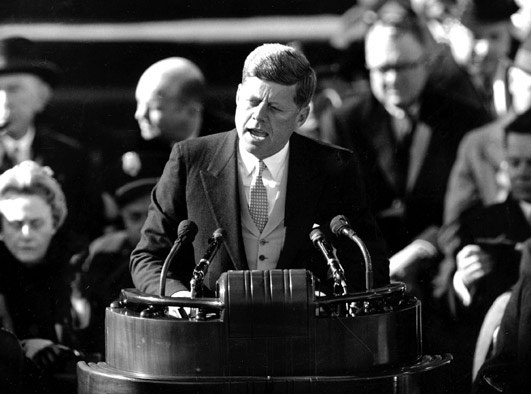
\includegraphics[width=0.6\textwidth]{ap_kennedy_050111_assh.jpg}\end{figure}
{\em Young, handsome, with a glamorous family in tow, John F. Kennedy embodied the fresh optimism that had marked the post-war decade. On January 20, 1961, Kennedy took the oath of office as the 35th President of the United States. The youngest president in United States history, he was the first man born in the 20th century to hold that office. Listening to his inaugural address, the nation felt that a new era and a “new frontier” were being ushered in.}

\vspace{10 mm}

Vice President Johnson, Mr. Speaker, Mr. Chief Justice, President Eisenhower, Vice President Nixon, President Truman, reverend clergy, fellow citizens:

We observe today not a victory of party, but a celebration of freedom — symbolizing an end, as well as a beginning — signifying renewal, as well as change. For I have sworn before you and Almighty God the same solemn oath our forebears prescribed nearly a century and three-quarters ago.

The world is very different now. For man holds in his mortal hands the power to abolish all forms of human poverty and all forms of human life. And yet the same revolutionary beliefs for which our forebears fought are still at issue around the globe — the belief that the rights of man come not from the generosity of the state, but from the hand of God.

We dare not forget today that we are the heirs of that first revolution. Let the word go forth from this time and place, to friend and foe alike, that the torch has been passed to a new generation of Americans — born in this century, tempered by war, disciplined by a hard and bitter peace, proud of our ancient heritage, and unwilling to witness or permit the slow undoing of those human rights to which this nation has always been committed, and to which we are committed today at home and around the world.

Let every nation know, whether it wishes us well or ill, that we shall pay any price, bear any burden, meet any hardship, support any friend, oppose any foe, to assure the survival and the success of liberty.

This much we pledge — and more.

To those old allies whose cultural and spiritual origins we share, we pledge the loyalty of faithful friends. United there is little we cannot do in a host of cooperative ventures. Divided there is little we can do — for we dare not meet a powerful challenge at odds and split asunder.

To those new states whom we welcome to the ranks of the free, we pledge our word that one form of colonial control shall not have passed away merely to be replaced by a far more iron tyranny. We shall not always expect to find them supporting our view. But we shall always hope to find them strongly supporting their own freedom — and to remember that, in the past, those who foolishly sought power by riding the back of the tiger ended up inside.

To those people in the huts and villages of half the globe struggling to break the bonds of mass misery, we pledge our best efforts to help them help themselves, for whatever period is required — not because the Communists may be doing it, not because we seek their votes, but because it is right. If a free society cannot help the many who are poor, it cannot save the few who are rich.

To our sister republics south of our border, we offer a special pledge: to convert our good words into good deeds, in a new alliance for progress, to assist free men and free governments in casting off the chains of poverty. But this peaceful revolution of hope cannot become the prey of hostile powers. Let all our neighbors know that we shall join with them to oppose aggression or subversion anywhere in the Americas. And let every other power know that this hemisphere intends to remain the master of its own house.

To that world assembly of sovereign states, the United Nations, our last best hope in an age where the instruments of war have far outpaced the instruments of peace, we renew our pledge of support — to prevent it from becoming merely a forum for invective, to strengthen its shield of the new and the weak, and to enlarge the area in which its writ may run.

Finally, to those nations who would make themselves our adversary, we offer not a pledge but a request: that both sides begin anew the quest for peace, before the dark powers of destruction unleashed by science engulf all humanity in planned or accidental self-destruction.

We dare not tempt them with weakness. For only when our arms are sufficient beyond doubt can we be certain beyond doubt that they will never be employed.

But neither can two great and powerful groups of nations take comfort from our present course — both sides overburdened by the cost of modern weapons, both rightly alarmed by the steady spread of the deadly atom, yet both racing to alter that uncertain balance of terror that stays the hand of mankind's final war.

So let us begin anew — remembering on both sides that civility is not a sign of weakness, and sincerity is always subject to proof. Let us never negotiate out of fear, but let us never fear to negotiate.

Let both sides explore what problems unite us instead of belaboring those problems which divide us.

Let both sides, for the first time, formulate serious and precise proposals for the inspection and control of arms, and bring the absolute power to destroy other nations under the absolute control of all nations.

Let both sides seek to invoke the wonders of science instead of its terrors. Together let us explore the stars, conquer the deserts, eradicate disease, tap the ocean depths, and encourage the arts and commerce.

Let both sides unite to heed, in all corners of the earth, the command of Isaiah — to “undo the heavy burdens, and [to] let the oppressed go free.”

And, if a beachhead of cooperation may push back the jungle of suspicion, let both sides join in creating a new endeavor — not a new balance of power, but a new world of law — where the strong are just, and the weak secure, and the peace preserved.

All this will not be finished in the first one hundred days. Nor will it be finished in the first one thousand days; nor in the life of this Administration; nor even perhaps in our lifetime on this planet. But let us begin.

In your hands, my fellow citizens, more than mine, will rest the final success or failure of our course. Since this country was founded, each generation of Americans has been summoned to give testimony to its national loyalty. The graves of young Americans who answered the call to service surround the globe.

Now the trumpet summons us again — not as a call to bear arms, though arms we need — not as a call to battle, though embattled we are — but a call to bear the burden of a long twilight struggle, year in and year out, “rejoicing in hope; patient in tribulation,” a struggle against the common enemies of man: tyranny, poverty, disease, and war itself.

Can we forge against these enemies a grand and global alliance, North and South, East and West, that can assure a more fruitful life for all mankind? Will you join in that historic effort?

In the long history of the world, only a few generations have been granted the role of defending freedom in its hour of maximum danger. I do not shrink from this responsibility — I welcome it. I do not believe that any of us would exchange places with any other people or any other generation. The energy, the faith, the devotion which we bring to this endeavor will light our country and all who serve it. And the glow from that fire can truly light the world.

And so, my fellow Americans, ask not what your country can do for you; ask what you can do for your country.

My fellow citizens of the world, ask not what America will do for you, but what together we can do for the freedom of man.

Finally, whether you are citizens of America or citizens of the world, ask of us here the same high standards of strength and sacrifice which we ask of you. With a good conscience our only sure reward, with history the final judge of our deeds, let us go forth to lead the land we love, asking His blessing and His help, but knowing that here on earth God's work must truly be our own.


\chapter{John F. Kennedy - The Decision to Go to the Moon}

\textbf{\Large{Huston, Texas -- May 25, 1961 }}

\vspace{10 mm}

\begin{figure}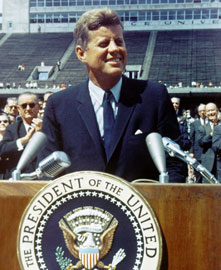
\includegraphics[width=0.6\textwidth]{kennedy_rice1.jpg}\end{figure}
{\em On April 12, 1961, the Soviets launched the first man into space. Khrushchev used this triumph as prime evidence of communism's superiority over decadent capitalism. Embarrassed, the United States feared it was falling behind the Soviet Union and losing the “space race.” After consulting with political and NASA officials, Kennedy decided it was time for America to boldly go where no man had gone before by putting a man on the moon. The feat would not only catapult the nation over the Soviet Union, but also allow man to more fully explore the mysteries of space. And this mission would be accomplished by the end of the 1960's. When was the last time a president had the cajones to publicly issue a straightforward, ambitious goal and set a timeline for its success?}

\vspace{10 mm}

President Pitzer, Mr. Vice President, Governor, Congressman Thomas, Senator Wiley, and Congressman Miller, Mr. Webb, Mr. Bell, scientists, distinguished guests, and ladies and gentlemen:

I appreciate your president having made me an honorary visiting professor, and I will assure you that my first lecture will be very brief.

I am delighted to be here and I'm particularly delighted to be here on this occasion.

We meet at a college noted for knowledge, in a city noted for progress, in a state noted for strength, and we stand in need of all three, for we meet in an hour of change and challenge, in a decade of hope and fear, in an age of both knowledge and ignorance. The greater our knowledge increases, the greater our ignorance unfolds.

Despite the striking fact that most of the scientists that the world has ever known are alive and working today, despite the fact that this Nation's own scientific manpower is doubling every 12 years in a rate of growth more than three times that of our population as a whole, despite that, the vast stretches of the unknown and the unanswered and the unfinished still far outstrip our collective comprehension.

No man can fully grasp how far and how fast we have come, but condense, if you will, the 50,000 years of man's recorded history in a time span of but a half-century. Stated in these terms, we know very little about the first 40 years, except at the end of them advanced man had learned to use the skins of animals to cover them. Then about 10 years ago, under this standard, man emerged from his caves to construct other kinds of shelter. Only five years ago man learned to write and use a cart with wheels. Christianity began less than two years ago. The printing press came this year, and then less than two months ago, during this whole 50-year span of human history, the steam engine provided a new source of power. Newton explored the meaning of gravity. Last month electric lights and telephones and automobiles and airplanes became available. Only last week did we develop penicillin and television and nuclear power, and now if America's new spacecraft succeeds in reaching Venus, we will have literally reached the stars before midnight tonight.

This is a breathtaking pace, and such a pace cannot help but create new ills as it dispels old, new ignorance, new problems, new dangers. Surely the opening vistas of space promise high costs and hardships, as well as high reward.

So it is not surprising that some would have us stay where we are a little longer to rest, to wait. But this city of Houston, this state of Texas, this country of the United States was not built by those who waited and rested and wished to look behind them. This country was conquered by those who moved forward–and so will space.

William Bradford, speaking in 1630 of the founding of the Plymouth Bay Colony, said that all great and honorable actions are accompanied with great difficulties, and both must be enterprised and overcome with answerable courage.

If this capsule history of our progress teaches us anything, it is that man, in his quest for knowledge and progress, is determined and cannot be deterred. The exploration of space will go ahead, whether we join in it or not, and it is one of the great adventures of all time, and no nation which expects to be the leader of other nations can expect to stay behind in this race for space.

Those who came before us made certain that this country rode the first waves of the industrial revolution, the first waves of modern invention, and the first wave of nuclear power, and this generation does not intend to founder in the backwash of the coming age of space. We mean to be a part of it–we mean to lead it. For the eyes of the world now look into space, to the moon and to the planets beyond, and we have vowed that we shall not see it governed by a hostile flag of conquest, but by a banner of freedom and peace. We have vowed that we shall not see space filled with weapons of mass destruction, but with instruments of knowledge and understanding.

Yet the vows of this Nation can only be fulfilled if we in this Nation are first, and, therefore, we intend to be first. In short, our leadership in science and industry, our hopes for peace and security, our obligations to ourselves as well as others, all require us to make this effort, to solve these mysteries, to solve them for the good of all men, and to become the world's leading space-faring nation.

We set sail on this new sea because there is new knowledge to be gained, and new rights to be won, and they must be won and used for the progress of all people. For space science, like nuclear science and all technology, has no conscience of its own. Whether it will become a force for good or ill depends on man, and only if the United States occupies a position of pre-eminence can we help decide whether this new ocean will be a sea of peace or a new terrifying theater of war. I do not say that we should or will go unprotected against the hostile misuse of space any more than we go unprotected against the hostile use of land or sea, but I do say that space can be explored and mastered without feeding the fires of war, without repeating the mistakes that man has made in extending his writ around this globe of ours.

There is no strife, no prejudice, no national conflict in outer space as yet. Its hazards are hostile to us all. Its conquest deserves the best of all mankind, and its opportunity for peaceful cooperation many never come again. But why, some say, the moon? Why choose this as our goal? And they may well ask why climb the highest mountain? Why, 35 years ago, fly the Atlantic? Why does Rice play Texas?

We choose to go to the moon. We choose to go to the moon in this decade and do the other things, not because they are easy, but because they are hard, because that goal will serve to organize and measure the best of our energies and skills, because that challenge is one that we are willing to accept, one we are unwilling to postpone, and one which we intend to win, and the others, too.

It is for these reasons that I regard the decision last year to shift our efforts in space from low to high gear as among the most important decisions that will be made during my incumbency in the office of the Presidency.

In the last 24 hours we have seen facilities now being created for the greatest and most complex exploration in man's history. We have felt the ground shake and the air shattered by the testing of a Saturn C-1 booster rocket, many times as powerful as the Atlas which launched John Glenn, generating power equivalent to 10,000 automobiles with their accelerators on the floor. We have seen the site where five F-1 rocket engines, each one as powerful as all eight engines of the Saturn combined, will be clustered together to make the advanced Saturn missile, assembled in a new building to be built at Cape Canaveral as tall as a 48 story structure, as wide as a city block, and as long as two lengths of this field.

Within these last 19 months at least 45 satellites have circled the earth. Some 40 of them were made in the United States of America and they were far more sophisticated and supplied far more knowledge to the people of the world than those of the Soviet Union.

The Mariner spacecraft now on its way to Venus is the most intricate instrument in the history of space science. The accuracy of that shot is comparable to firing a missile from Cape Canaveral and dropping it in this stadium between the 40-yard lines.

Transit satellites are helping our ships at sea to steer a safer course. Tiros satellites have given us unprecedented warnings of hurricanes and storms, and will do the same for forest fires and icebergs.

We have had our failures, but so have others, even if they do not admit them. And they may be less public.

To be sure, we are behind, and will be behind for some time in manned flight. But we do not intend to stay behind, and in this decade, we shall make up and move ahead.

The growth of our science and education will be enriched by new knowledge of our universe and environment, by new techniques of learning and mapping and observation, by new tools and computers for industry, medicine, the home as well as the school. Technical institutions, such as Rice, will reap the harvest of these gains.

And finally, the space effort itself, while still in its infancy, has already created a great number of new companies, and tens of thousands of new jobs. Space and related industries are generating new demands in investment and skilled personnel, and this city and this state, and this region, will share greatly in this growth. What was once the furthest outpost on the old frontier of the West will be the furthest outpost on the new frontier of science and space. Houston, your city of Houston, with its Manned Spacecraft Center, will become the heart of a large scientific and engineering community. During the next 5 years the National Aeronautics and Space Administration expects to double the number of scientists and engineers in this area, to increase its outlays for salaries and expenses to \$60 million a year; to invest some \$200 million in plant and laboratory facilities; and to direct or contract for new space efforts over \$1 billion from this center in this city.

To be sure, all this costs us all a good deal of money. This year's space budget is three times what it was in January 1961, and it is greater than the space budget of the previous eight years combined. That budget now stands at \$5,400 million a year–a staggering sum, though somewhat less than we pay for cigarettes and cigars every year. Space expenditures will soon rise some more, from 40 cents per person per week to more than 50 cents a week for every man, woman and child in the United States, for we have given this program a high national priority–even though I realize that this is in some measure an act of faith and vision, for we do not now know what benefits await us. But if I were to say, my fellow citizens, that we shall send to the moon, 240,000 miles away from the control station in Houston, a giant rocket more than 300 feet tall, the length of this football field, made of new metal alloys, some of which have not yet been invented, capable of standing heat and stresses several times more than have ever been experienced, fitted together with a precision better than the finest watch, carrying all the equipment needed for propulsion, guidance, control, communications, food and survival, on an untried mission, to an unknown celestial body, and then return it safely to earth, re-entering the atmosphere at speeds of over 25,000 miles per hour, causing heat about half that of the temperature of the sun–almost as hot as it is here today–and do all this, and do it right, and do it first before this decade is out–then we must be bold.

I'm the one who is doing all the work, so we just want you to stay cool for a minute. [laughter]

However, I think we're going to do it, and I think that we must pay what needs to be paid. I don't think we ought to waste any money, but I think we ought to do the job. And this will be done in the decade of the Sixties. It may be done while some of you are still here at school at this college and university. It will be done during the terms of office of some of the people who sit here on this platform. But it will be done. And it will be done before the end of this decade.

And I am delighted that this university is playing a part in putting a man on the moon as part of a great national effort of the United States of America.

Many years ago the great British explorer George Mallory, who was to die on Mount Everest, was asked why did he want to climb it. He said, “Because it is there.”

Well, space is there, and we're going to climb it, and the moon and the planets are there, and new hopes for knowledge and peace are there. And, therefore, as we set sail we ask God's blessing on the most hazardous and dangerous and greatest adventure on which man has ever embarked.

Thank you.


\chapter{General Douglas MacArthur - Duty, Honor, Country}

\textbf{\Large{West Point, New York -- May 12, 1962 }}

\vspace{10 mm}

\begin{figure}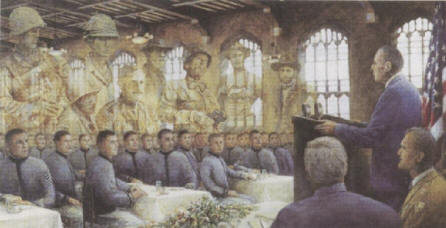
\includegraphics[width=0.6\textwidth]{douglaswestpointsteucke.jpg}\end{figure}
{\em General Douglas MacArthur, General of the Army and a man who fought in three wars, knew something of “Duty, Honor, Country.” In 1962, MacArthur was in the twilight of his life and came to West Point to accept the Sylvanus Thayer Award and participate in his final cadet roll call. His address reflects upon and celebrates the brave and courageous men who came before, men he personally led, men who embodied “Duty, Honor, Country.”

There are many great speeches in this list, but I hope you will pause to read the entirety of this one. Picking an excerpt was quite difficult, as so many of the passages are inspiring. A must read for all men.}

\vspace{10 mm}

General Westmoreland, General Grove, distinguished guests, and gentlemen of the Corps!

As I was leaving the hotel this morning, a doorman asked me, “Where are you bound for, General?” And when I replied, “West Point,” he remarked, “Beautiful place. Have you ever been there before?”

No human being could fail to be deeply moved by such a tribute as this [Thayer Award]. Coming from a profession I have served so long, and a people I have loved so well, it fills me with an emotion I cannot express. But this award is not intended primarily to honor a personality, but to symbolize a great moral code — the code of conduct and chivalry of those who guard this beloved land of culture and ancient descent. That is the animation of this medallion. For all eyes and for all time, it is an expression of the ethics of the American soldier. That I should be integrated in this way with so noble an ideal arouses a sense of pride and yet of humility which will be with me always

Duty, Honor, Country: Those three hallowed words reverently dictate what you ought to be, what you can be, what you will be. They are your rallying points: to build courage when courage seems to fail; to regain faith when there seems to be little cause for faith; to create hope when hope becomes forlorn.

Unhappily, I possess neither that eloquence of diction, that poetry of imagination, nor that brilliance of metaphor to tell you all that they mean.

The unbelievers will say they are but words, but a slogan, but a flamboyant phrase. Every pedant, every demagogue, every cynic, every hypocrite, every troublemaker, and I am sorry to say, some others of an entirely different character, will try to downgrade them even to the extent of mockery and ridicule.

But these are some of the things they do. They build your basic character. They mold you for your future roles as the custodians of the nation's defense. They make you strong enough to know when you are weak, and brave enough to face yourself when you are afraid. They teach you to be proud and unbending in honest failure, but humble and gentle in success; not to substitute words for actions, not to seek the path of comfort, but to face the stress and spur of difficulty and challenge; to learn to stand up in the storm but to have compassion on those who fall; to master yourself before you seek to master others; to have a heart that is clean, a goal that is high; to learn to laugh, yet never forget how to weep; to reach into the future yet never neglect the past; to be serious yet never to take yourself too seriously; to be modest so that you will remember the simplicity of true greatness, the open mind of true wisdom, the meekness of true strength. They give you a temper of the will, a quality of the imagination, a vigor of the emotions, a freshness of the deep springs of life, a temperamental predominance of courage over timidity, of an appetite for adventure over love of ease. They create in your heart the sense of wonder, the unfailing hope of what next, and the joy and inspiration of life. They teach you in this way to be an officer and a gentleman.

And what sort of soldiers are those you are to lead? Are they reliable? Are they brave? Are they capable of victory? Their story is known to all of you. It is the story of the American man-at-arms. My estimate of him was formed on the battlefield many, many years ago, and has never changed. I regarded him then as I regard him now — as one of the world's noblest figures, not only as one of the finest military characters, but also as one of the most stainless. His name and fame are the birthright of every American citizen. In his youth and strength, his love and loyalty, he gave all that mortality can give.

He needs no eulogy from me or from any other man. He has written his own history and written it in red on his enemy's breast. But when I think of his patience under adversity, of his courage under fire, and of his modesty in victory, I am filled with an emotion of admiration I cannot put into words. He belongs to history as furnishing one of the greatest examples of successful patriotism. He belongs to posterity as the instructor of future generations in the principles of liberty and freedom. He belongs to the present, to us, by his virtues and by his achievements. In 20 campaigns, on a hundred battlefields, around a thousand campfires, I have witnessed that enduring fortitude, that patriotic self-abnegation, and that invincible determination which have carved his statue in the hearts of his people. From one end of the world to the other he has drained deep the chalice of courage.

As I listened to those songs [of the glee club], in memory's eye I could see those staggering columns of the First World War, bending under soggy packs, on many a weary march from dripping dusk to drizzling dawn, slogging ankle-deep through the mire of shell-shocked roads, to form grimly for the attack, blue-lipped, covered with sludge and mud, chilled by the wind and rain, driving home to their objective, and for many, to the judgment seat of  God.

I do not know the dignity of their birth, but I do know the glory of their death. They died unquestioning, uncomplaining, with faith in their hearts, and on their lips the hope that we would go on to victory. Always, for them: Duty, Honor, Country; always their blood and sweat and tears, as we sought the way and the light and the truth.

And 20 years after, on the other side of the globe, again the filth of murky foxholes, the stench of ghostly trenches, the slime of dripping dugouts; those boiling suns of relentless heat, those torrential rains of devastating storms; the loneliness and utter desolation of jungle trails; the bitterness of long separation from those they loved and cherished; the deadly pestilence of tropical disease; the horror of stricken areas of war; their resolute and determined defense, their swift and sure attack, their indomitable purpose, their complete and decisive victory — always victory. Always through the bloody haze of their last reverberating shot, the vision of gaunt, ghastly men reverently following your password of: Duty, Honor, Country.

The code which those words perpetuate embraces the highest moral laws and will stand the test of any ethics or philosophies ever promulgated for the uplift of mankind. Its requirements are for the things that are right, and its restraints are from the things that are wrong.

The soldier, above all other men, is required to practice the greatest act of religious training — sacrifice.

In battle and in the face of danger and death, he discloses those divine attributes which his Maker gave when he created man in his own image. No physical courage and no brute instinct can take the place of the Divine help which alone can sustain him.

However horrible the incidents of war may be, the soldier who is called upon to offer and to give his life for his country is the noblest development of mankind.

You now face a new world — a world of change. The thrust into outer space of the satellite, spheres, and missiles mark the beginning of another epoch in the long story of mankind. In the five or more billions of years the scientists tell us it has taken to form the earth, in the three or more billion years of development of the human race, there has never been a more abrupt or staggering evolution. We deal now not with things of this world alone, but with the illimitable distances and as yet unfathomed mysteries of the universe. We are reaching out for a new and boundless frontier.

We speak in strange terms: of harnessing the cosmic energy; of making winds and tides work for us; of creating unheard synthetic materials to supplement or even replace our old standard basics; to purify sea water for our drink; of mining ocean floors for new fields of wealth and food; of disease preventatives to expand life into the hundreds of years; of controlling the weather for a more equitable distribution of heat and cold, of rain and shine; of space ships to the moon; of the primary target in war, no longer limited to the armed forces of an enemy, but instead to include his civil populations; of ultimate conflict between a united human race and the sinister forces of some other planetary galaxy; of such dreams and fantasies as to make life the most exciting of all time.

And through all this welter of change and development, your mission remains fixed, determined, inviolable: it is to win our wars.

Everything else in your professional career is but corollary to this vital dedication. All other public purposes, all other public projects, all other public needs, great or small, will find others for their accomplishment. But you are the ones who are trained to fight. Yours is the profession of arms,  the will to win, the sure knowledge that in war there is no substitute for victory; that if you lose, the nation will be destroyed; that the very obsession of your public service must be: Duty, Honor, Country.

Others will debate the controversial issues, national and international, which divide men's minds; but serene, calm, aloof, you stand as the Nation's war-guardian, as its lifeguard from the raging tides of international conflict, as its gladiator in the arena of battle. For a century and a half you have defended, guarded, and protected its hallowed traditions of liberty and freedom, of right and justice.

Let civilian voices argue the merits or demerits of our processes of government; whether our strength is being sapped by deficit financing, indulged in too long, by federal paternalism grown too mighty, by power groups grown too arrogant, by politics grown too corrupt, by crime grown too rampant, by morals grown too low, by taxes grown too high, by extremists grown too violent; whether our personal liberties are as thorough and complete as they should be. These great national problems are not for your professional participation or military solution. Your guidepost stands out like a ten-fold beacon in the night: Duty, Honor, Country.

You are the leaven which binds together the entire fabric of our national system of defense. From your ranks come the great captains who hold the nation's destiny in their hands the moment the war tocsin sounds. The Long Gray Line has never failed us. Were you to do so, a million ghosts in olive drab, in brown khaki, in blue and gray, would rise from their white crosses thundering those magic words: Duty, Honor, Country.

This does not mean that you are war mongers.

On the contrary, the soldier, above all other people, prays for peace, for he must suffer and bear the deepest wounds and scars of war.

But always in our ears ring the ominous words of Plato, that wisest of all philosophers: “Only the dead have seen the end of war.”

The shadows are lengthening for me. The twilight is here. My days of old have vanished, tone and tint. They have gone glimmering through the dreams of things that were. Their memory is one of wondrous beauty, watered by tears, and coaxed and caressed by the smiles of yesterday. I listen vainly, but with thirsty ears, for the witching melody of faint bugles blowing reveille, of far drums beating the long roll. In my dreams I hear again the crash of guns, the rattle of musketry, the strange, mournful mutter of the battlefield.

But in the evening of my memory, always I come back to West Point.

Always there echoes and re-echoes: Duty, Honor, Country.

Today marks my final roll call with you, but I want you to know that when I cross the river my last conscious thoughts will be of The Corps, and The Corps, and The Corps.

I bid you farewell.


\chapter{Martin Luther King Jr. - I Have a Dream}

\textbf{\Large{Washington D.C. -- August 28, 1963 }}

\vspace{10 mm}

\begin{figure}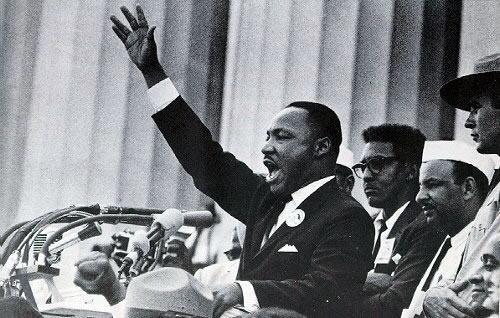
\includegraphics[width=0.6\textwidth]{i_have_a_dream.jpg}\end{figure}
{\em Martin Luther King Jr.'s “I Have a Dream Speech” is hands down one of the greatest, if not the greatest, pieces of oratory in American history. King's charisma, skills in rhetoric, and passion, place him in a league of his own. A century after slavery ended, a century after African-Americans were promised full equality, black children were being hosed down in the streets, spat upon, bused to separate schools, turned away from restaurants, and denied treatment as full human beings. In this midst of this egregious track record, Dr. King voiced a clear, compelling message of hope, a dream that things would not always be as they were, and that a new day was coming.

Many people have seen excerpts of the speech, but a surprisingly number of adults my age I have never sat down and watched the speech in its entirety. I challenge you to do just that. It is just as electrifying and moving today as it was in 1963.}

\vspace{10 mm}

I am happy to join with you today in what will go down in history as the greatest demonstration for freedom in the history of our nation.

Five score years ago, a great American, in whose symbolic shadow we stand today, signed the Emancipation Proclamation. This momentous decree came as a great beacon light of hope to millions of Negro slaves who had been seared in the flames of withering injustice. It came as a joyous daybreak to end the long night of their captivity.

But one hundred years later, the Negro still is not free. One hundred years later, the life of the Negro is still sadly crippled by the manacles of segregation and the chains of discrimination. One hundred years later, the Negro lives on a lonely island of poverty in the midst of a vast ocean of material prosperity. One hundred years later, the Negro is still languished in the corners of American society and finds himself an exile in his own land. And so we've come here today to dramatize a shameful condition.

In a sense we've come to our nation's capital to cash a check. When the architects of our republic wrote the magnificent words of the Constitution and the Declaration of Independence, they were signing a promissory note to which every American was to fall heir. This note was a promise that all men, yes, black men as well as white men, would be guaranteed the “unalienable Rights” of “Life, Liberty and the pursuit of Happiness.” It is obvious today that America has defaulted on this promissory note, insofar as her citizens of color are concerned. Instead of honoring this sacred obligation, America has given the Negro people a bad check, a check which has come back marked “insufficient funds.”

But we refuse to believe that the bank of justice is bankrupt. We refuse to believe that there are insufficient funds in the great vaults of opportunity of this nation. And so, we've come to cash this check, a check that will give us upon demand the riches of freedom and the security of justice.

We have also come to this hallowed spot to remind America of the fierce urgency of Now. This is no time to engage in the luxury of cooling off or to take the tranquilizing drug of gradualism. Now is the time to make real the promises of democracy. Now is the time to rise from the dark and desolate valley of segregation to the sunlit path of racial justice. Now is the time to lift our nation from the quicksands of racial injustice to the solid rock of brotherhood. Now is the time to make justice a reality for all of God's children.

It would be fatal for the nation to overlook the urgency of the moment. This sweltering summer of the Negro's legitimate discontent will not pass until there is an invigorating autumn of freedom and equality. Nineteen sixty-three is not an end, but a beginning. And those who hope that the Negro needed to blow off steam and will now be content will have a rude awakening if the nation returns to business as usual. And there will be neither rest nor tranquility in America until the Negro is granted his citizenship rights. The whirlwinds of revolt will continue to shake the foundations of our nation until the bright day of justice emerges.

But there is something that I must say to my people, who stand on the warm threshold which leads into the palace of justice: In the process of gaining our rightful place, we must not be guilty of wrongful deeds. Let us not seek to satisfy our thirst for freedom by drinking from the cup of bitterness and hatred. We must forever conduct our struggle on the high plane of dignity and discipline. We must not allow our creative protest to degenerate into physical violence. Again and again, we must rise to the majestic heights of meeting physical force with soul force.

The marvelous new militancy which has engulfed the Negro community must not lead us to a distrust of all white people, for many of our white brothers, as evidenced by their presence here today, have come to realize that their destiny is tied up with our destiny. And they have come to realize that their freedom is inextricably bound to our freedom.

We cannot walk alone.

And as we walk, we must make the pledge that we shall always march ahead.

We cannot turn back.

There are those who are asking the devotees of civil rights, “When will you be satisfied?” We can never be satisfied as long as the Negro is the victim of the unspeakable horrors of police brutality. We can never be satisfied as long as our bodies, heavy with the fatigue of travel, cannot gain lodging in the motels of the highways and the hotels of the cities. We cannot be satisfied as long as the negro's basic mobility is from a smaller ghetto to a larger one. We can never be satisfied as long as our children are stripped of their self-hood and robbed of their dignity by a sign stating: “For Whites Only.” We cannot be satisfied as long as a Negro in Mississippi cannot vote and a Negro in New York believes he has nothing for which to vote. No, no, we are not satisfied, and we will not be satisfied until “justice rolls down like waters, and righteousness like a mighty stream.”

I am not unmindful that some of you have come here out of great trials and tribulations. Some of you have come fresh from narrow jail cells. And some of you have come from areas where your quest — quest for freedom left you battered by the storms of persecution and staggered by the winds of police brutality. You have been the veterans of creative suffering. Continue to work with the faith that unearned suffering is redemptive. Go back to Mississippi, go back to Alabama, go back to South Carolina, go back to Georgia, go back to Louisiana, go back to the slums and ghettos of our northern cities, knowing that somehow this situation can and will be changed.

Let us not wallow in the valley of despair, I say to you today, my friends.

And so even though we face the difficulties of today and tomorrow, I still have a dream. It is a dream deeply rooted in the American dream.

I have a dream that one day this nation will rise up and live out the true meaning of its creed: “We hold these truths to be self-evident, that all men are created equal.”

I have a dream that one day on the red hills of Georgia, the sons of former slaves and the sons of former slave owners will be able to sit down together at the table of brotherhood.

I have a dream that one day even the state of Mississippi, a state sweltering with the heat of injustice, sweltering with the heat of oppression, will be transformed into an oasis of freedom and justice.

I have a dream that my four little children will one day live in a nation where they will not be judged by the color of their skin but by the content of their character.

I have a dream today!

I have a dream that one day, down in Alabama, with its vicious racists, with its governor having his lips dripping with the words of “interposition” and “nullification” — one day right there in Alabama little black boys and black girls will be able to join hands with little white boys and white girls as sisters and brothers.

I have a dream today!

I have a dream that one day every valley shall be exalted, and every hill and mountain shall be made low, the rough places will be made plain, and the crooked places will be made straight; “and the glory of the Lord shall be revealed and all flesh shall see it together.”

This is our hope, and this is the faith that I go back to the South with.

With this faith, we will be able to hew out of the mountain of despair a stone of hope. With this faith, we will be able to transform the jangling discords of our nation into a beautiful symphony of brotherhood. With this faith, we will be able to work together, to pray together, to struggle together, to go to jail together, to stand up for freedom together, knowing that we will be free one day.

And this will be the day – this will be the day when all of God's children will be able to sing with new meaning:

\begin{quote}My country 'tis of thee, sweet land of liberty, of thee I sing.\end{quote}

\begin{quote}Land where my fathers died, land of the Pilgrim's pride,\end{quote}

\begin{quote}From every mountainside, let freedom ring!\end{quote}

And if America is to be a great nation, this must become true.

And so let freedom ring from the prodigious hilltops of New Hampshire.

\begin{quote}Let freedom ring from the mighty mountains of New York.\end{quote}

\begin{quote}Let freedom ring from the heightening Alleghenies of Pennsylvania.\end{quote}

\begin{quote}Let freedom ring from the snow-capped Rockies of Colorado.\end{quote}

\begin{quote}Let freedom ring from the curvaceous slopes of California.\end{quote}

But not only that:

\begin{quote}Let freedom ring from Stone Mountain of Georgia.\end{quote}

\begin{quote}Let freedom ring from Lookout Mountain of Tennessee.\end{quote}

\begin{quote}Let freedom ring from every hill and molehill of Mississippi.\end{quote}

\begin{quote}From every mountainside, let freedom ring.\end{quote}

And when this happens, when we allow freedom ring, when we let it ring from every village and every hamlet, from every state and every city, we will be able to speed up that day when all of God's children, black men and white men, Jews and Gentiles, Protestants and Catholics, will be able to join hands and sing in the words of the old Negro spiritual:

\begin{quote}Free at last! Free at last!\end{quote}

\begin{quote}Thank God Almighty, we are free at last!\end{quote}


\chapter{Ronald Reagan - 40th Aniversary of D-Day}

\textbf{\Large{Pointe du Hoc, France -- June 06, 1984 }}

\vspace{10 mm}

\begin{figure}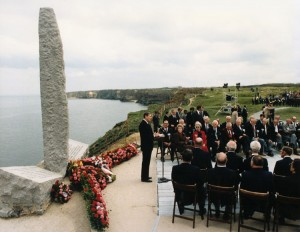
\includegraphics[width=0.6\textwidth]{president_reagan_giving_speech_on_the_40th_anniversary_of_d-day_at_pointe_du_hoc_normandy_france_1984-300x232.jpg}\end{figure}
{\em What the Army Rangers did on D-Day at Pointe Du Hoc is a tale every man worth his salt should be familiar with. Pointe du Hoc was a sheer 100 foot cliff located in-between Omaha and Utah beaches. Perched atop the cliff sat six casemates capable of being manned, armed, and taking out the men on the beaches. As the Germans fired upon them, the Rangers scaled the cliff using ropes and ladders, found the guns (which had been moved from the casemates) and destroyed them. Without reinforcements for two days, the Rangers alone held their position and fended off German counterattacks. These skirmishes proved deadly; only 90 of the original 225 Ranger landing force survived.

On the 40th anniversary of D-Day, President Reagan gave a moving tribute to these men, many of whom were present at the occasion.}

\vspace{10 mm}

We're here to mark that day in history when the Allied armies joined in battle to reclaim this continent to liberty. For four long years, much of Europe had been under a terrible shadow. Free nations had fallen, Jews cried out in the camps, millions cried out for liberation. Europe was enslaved and the world prayed for its rescue. Here, in Normandy, the rescue began. Here, the Allies stood and fought against tyranny, in a giant undertaking unparalleled in human history.

We stand on a lonely, windswept point on the northern shore of France. The air is soft, but forty years ago at this moment, the air was dense with smoke and the cries of men, and the air was filled with the crack of rifle fire and the roar of cannon. At dawn, on the morning of the 6th of June, 1944, two hundred and twenty-five Rangers jumped off the British landing craft and ran to the bottom of these cliffs.

Their mission was one of the most difficult and daring of the invasion: to climb these sheer and desolate cliffs and take out the enemy guns. The Allies had been told that some of the mightiest of these guns were here, and they would be trained on the beaches to stop the Allied advance.

The Rangers looked up and saw the enemy soldiers at the edge of the cliffs, shooting down at them with machine guns and throwing grenades. And the American Rangers began to climb. They shot rope ladders over the face of these cliffs and began to pull themselves up. When one Ranger fell, another would take his place. When one rope was cut, a Ranger would grab another and begin his climb again. They climbed, shot back, and held their footing. Soon, one by one, the Rangers pulled themselves over the top, and in seizing the firm land at the top of these cliffs, they began to seize back the continent of Europe. Two hundred and twenty-five came here. After two days of fighting, only ninety could still bear arms.

And behind me is a memorial that symbolizes the Ranger daggers that were thrust into the top of these cliffs. And before me are the men who put them there. These are the boys of Pointe du Hoc. These are the men who took the cliffs. These are the champions who helped free a continent. And these are the heroes who helped end a war. Gentlemen, I look at you and I think of the words of Stephen Spender's poem. You are men who in your “lives fought for life and left the vivid air signed with your honor.”

I think I know what you may be thinking right now — thinking “we were just part of a bigger effort; everyone was brave that day.” Well everyone was. Do you remember the story of Bill Millin of the 51st Highlanders? Forty years ago today, British troops were pinned down near a bridge, waiting desperately for help. Suddenly, they heard the sound of bagpipes, and some thought they were dreaming. Well, they weren't. They looked up and saw Bill Millin with his bagpipes, leading the reinforcements and ignoring the smack of the bullets into the ground around him.

Lord Lovat was with him — Lord Lovat of Scotland, who calmly announced when he got to the bridge, “Sorry, I'm a few minutes late,” as if he'd been delayed by a traffic jam, when in truth he'd just come from the bloody fighting on Sword Beach, which he and his men had just taken.

There was the impossible valor of the Poles, who threw themselves between the enemy and the rest of Europe as the invasion took hold; and the unsurpassed courage of the Canadians who had already seen the horrors of war on this coast. They knew what awaited them there, but they would not be deterred. And once they hit Juno Beach, they never looked back.

All of these men were part of a roll call of honor with names that spoke of a pride as bright as the colors they bore; The Royal Winnipeg Rifles, Poland's 24th Lancers, the Royal Scots' Fusiliers, the Screaming Eagles, the Yeomen of England's armored divisions, the forces of Free France, the Coast Guard's “Matchbox Fleet,” and you, the American Rangers.

Forty summers have passed since the battle that you fought here. You were young the day you took these cliffs; some of you were hardly more than boys, with the deepest joys of life before you. Yet you risked everything here. Why? Why did you do it? What impelled you to put aside the instinct for self-preservation and risk your lives to take these cliffs? What inspired all the men of the armies that met here? We look at you, and somehow we know the answer. It was faith and belief. It was loyalty and love.

The men of Normandy had faith that what they were doing was right, faith that they fought for all humanity, faith that a just God would grant them mercy on this beachhead, or on the next. It was the deep knowledge — and pray God we have not lost it — that there is a profound moral difference between the use of force for liberation and the use of force for conquest. You were here to liberate, not to conquer, and so you and those others did not doubt your cause. And you were right not to doubt.

You all knew that some things are worth dying for. One's country is worth dying for, and democracy is worth dying for, because it's the most deeply honorable form of government ever devised by man. All of you loved liberty. All of you were willing to fight tyranny, and you knew the people of your countries were behind you.

The Americans who fought here that morning knew word of the invasion was spreading through the darkness back home. They fought — or felt in their hearts, though they couldn't know in fact, that in Georgia they were filling the churches at 4:00 am. In Kansas they were kneeling on their porches and praying. And in Philadelphia they were ringing the Liberty Bell.

Something else helped the men of D-day; their rock-hard belief that Providence would have a great hand in the events that would unfold here; that God was an ally in this great cause. And so, the night before the invasion, when Colonel Wolverton asked his parachute troops to kneel with him in prayer, he told them: “Do not bow your heads, but look up so you can see God and ask His blessing in what we're about to do.” Also, that night, General Matthew Ridgway on his cot, listening in the darkness for the promise God made to Joshua: “I will not fail thee nor forsake thee.”

These are the things that impelled them; these are the things that shaped the unity of the Allies.

When the war was over, there were lives to be rebuilt and governments to be returned to the people. There were nations to be reborn. Above all, there was a new peace to be assured. These were huge and daunting tasks. But the Allies summoned strength from the faith, belief, loyalty, and love of those who fell here. They rebuilt a new Europe together. There was first a great reconciliation among those who had been enemies, all of whom had suffered so greatly. The United States did its part, creating the Marshall Plan to help rebuild our allies and our former enemies. The Marshall Plan led to the Atlantic alliance — a great alliance that serves to this day as our shield for freedom, for prosperity, and for peace.

In spite of our great efforts and successes, not all that followed the end of the war was happy or planned. Some liberated countries were lost. The great sadness of this loss echoes down to our own time in the streets of Warsaw, Prague, and East Berlin. The Soviet troops that came to the center of this continent did not leave when peace came. They're still there, uninvited, unwanted, unyielding, almost forty years after the war. Because of this, allied forces still stand on this continent. Today, as forty years ago, our armies are here for only one purpose: to protect and defend democracy. The only territories we hold are memorials like this one and graveyards where our heroes rest.

We in America have learned bitter lessons from two world wars. It is better to be here ready to protect the peace, than to take blind shelter across the sea, rushing to respond only after freedom is lost. We've learned that isolationism never was and never will be an acceptable response to tyrannical governments with an expansionist intent. But we try always to be prepared for peace, prepared to deter aggression, prepared to negotiate the reduction of arms, and yes, prepared to reach out again in the spirit of reconciliation. In truth, there is no reconciliation we would welcome more than a reconciliation with the Soviet Union, so, together, we can lessen the risks of war, now and forever.

It's fitting to remember here the great losses also suffered by the Russian people during World War II. Twenty million perished, a terrible price that testifies to all the world the necessity of ending war. I tell you from my heart that we in the United States do not want war. We want to wipe from the face of the earth the terrible weapons that man now has in his hands. And I tell you, we are ready to seize that beachhead. We look for some sign from the Soviet Union that they are willing to move forward, that they share our desire and love for peace, and that they will give up the ways of conquest. There must be a changing there that will allow us to turn our hope into action.

We will pray forever that someday that changing will come. But for now, particularly today, it is good and fitting to renew our commitment to each other, to our freedom, and to the alliance that protects it.

We're bound today by what bound us 40 years ago, the same loyalties, traditions, and beliefs. We're bound by reality. The strength of America's allies is vital to the United States, and the American security guarantee is essential to the continued freedom of Europe's democracies. We were with you then; we're with you now. Your hopes are our hopes, and your destiny is our destiny.

Here, in this place where the West held together, let us make a vow to our dead. Let us show them by our actions that we understand what they died for. Let our actions say to them the words for which Matthew Ridgway listened: “I will not fail thee nor forsake thee.”

Strengthened by their courage and heartened by their value [valor] and borne by their memory, let us continue to stand for the ideals for which they lived and died.

Thank you very much, and God bless you all.


\chapter{Ronald Reagan - Address to the Nation on the Challenger}

\textbf{\Large{Washington D.C. -- January 28, 1986 }}

\vspace{10 mm}

\begin{figure}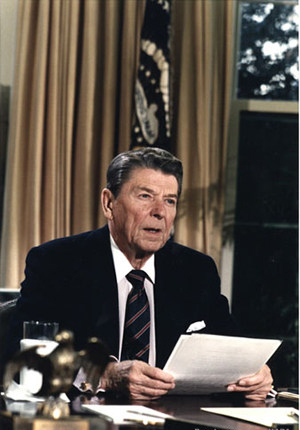
\includegraphics[width=0.6\textwidth]{ronaldreagan_challengerovaloffice.jpg}\end{figure}
{\em On January 28, 1986, millions of Americans, many of them schoolchildren watching from their classroom desks, tuned in to see 7 Americans, including Christa McAuliffe, a 37 year old schoolteacher and the first ever “civilian astronaut,” lift off in the space shuttle Challenger. Just 73 seconds later, the shuttle was consumed in a fireball. All seven aboard perished. These were the first deaths of American astronauts while in flight, and the nation was shocked and heartbroken by the tragedy. Just a few hours after the disaster, President Ronald Reagan took to the radio and airwaves, honoring these “pioneers” and offering comfort and assurance to a rattled people.}

\vspace{10 mm}

Ladies and Gentlemen, I'd planned to speak to you tonight to report on the state of the Union, but the events of earlier today have led me to change those plans. Today is a day for mourning and remembering. Nancy and I are pained to the core by the tragedy of the shuttle Challenger. We know we share this pain with all of the people of our country. This is truly a national loss.

Nineteen years ago, almost to the day, we lost three astronauts in a terrible accident on the ground. But, we've never lost an astronaut in flight; we've never had a tragedy like this. And perhaps we've forgotten the courage it took for the crew of the shuttle; but they, the Challenger Seven, were aware of the dangers, but overcame them and did their jobs brilliantly. We mourn seven heroes: Michael Smith, Dick Scobee, Judith Resnik, Ronald McNair, Ellison Onizuka, Gregory Jarvis, and Christa McAuliffe. We mourn their loss as a nation together.

For the families of the seven, we cannot bear, as you do, the full impact of this tragedy. But we feel the loss, and we're thinking about you so very much. Your loved ones were daring and brave, and they had that special grace, that special spirit that says, ‘Give me a challenge and I'll meet it with joy.' They had a hunger to explore the universe and discover its truths. They wished to serve, and they did. They served all of us.

We've grown used to wonders in this century. It's hard to dazzle us. But for twenty-five years the United States space program has been doing just that. We've grown used to the idea of space, and perhaps we forget that we've only just begun. We're still pioneers. They, the members of the Challenger crew, were pioneers.

And I want to say something to the schoolchildren of America who were watching the live coverage of the shuttle's takeoff. I know it is hard to understand, but sometimes painful things like this happen. It's all part of the process of exploration and discovery. It's all part of taking a chance and expanding man's horizons. The future doesn't belong to the fainthearted; it belongs to the brave. The Challenger crew was pulling us into the future, and we'll continue to follow them.

I've always had great faith in and respect for our space program, and what happened today does nothing to diminish it. We don't hide our space program. We don't keep secrets and cover things up. We do it all up front and in public. That's the way freedom is, and we wouldn't change it for a minute. We'll continue our quest in space. There will be more shuttle flights and more shuttle crews and, yes, more volunteers, more civilians, more teachers in space. Nothing ends here; our hopes and our journeys continue. I want to add that I wish I could talk to every man and woman who works for NASA or who worked on this mission and tell them: “Your dedication and professionalism have moved and impressed us for decades. And we know of your anguish. We share it.”

There's a coincidence today. On this day 390 years ago, the great explorer Sir Francis Drake died aboard ship off the coast of Panama. In his lifetime the great frontiers were the oceans, and a historian later said, ‘He lived by the sea, died on it, and was buried in it.' Well, today we can say of the Challenger crew: Their dedication was, like Drake's, complete.

The crew of the space shuttle Challenger honoured us by the manner in which they lived their lives. We will never forget them, nor the last time we saw them, this morning, as they prepared for the journey and waved goodbye and ‘slipped the surly bonds of earth' to ‘touch the face of God.'

Thank you.


\chapter{Ronald Reagan - Remarks at the Brandenburg Gate}

\textbf{\Large{Brandenburg Gate, Berlin -- June 12, 1987 }}

\vspace{10 mm}

\begin{figure}
\includegraphics[width=0.6\textwidth]{reagan-at-brandenburg.jpg}\end{figure}
{\em Since the end of World War II, Germany had been a divided country, the West free and democratic, the East under authoritarian communist control. When President Reagan took office, he was committed not only to uniting that country, but to bringing down the entire “Evil Empire.” While the importance of Reagan's role in successfully doing so is endlessly debated, it beyond dispute that he exerted some influence in bringing the Cold War to an end. There is no more memorable and symbolic moment of this influence then when Reagan stood at the Berlin wall, the most visible symbol of the “Iron Curtain,” and challenged Gorbachev to “tear down this wall!”}

\vspace{10 mm}

Thank you. Thank you, very much.

Chancellor Kohl, Governing Mayor Diepgen, ladies and gentlemen: Twenty four years ago, President John F. Kennedy visited Berlin, and speaking to the people of this city and the world at the city hall. Well since then two other presidents have come, each in his turn to Berlin. And today, I, myself, make my second visit to your city.

We come to Berlin, we American Presidents, because it's our duty to speak in this place of freedom. But I must confess, we're drawn here by other things as well; by the feeling of history in this city — more than 500 years older than our own nation; by the beauty of the Grunewald and the Tiergarten; most of all, by your courage and determination. Perhaps the composer, Paul Linke, understood something about American Presidents. You see, like so many Presidents before me, I come here today because wherever I go, whatever I do: “Ich hab noch einen Koffer in Berlin” [I still have a suitcase in Berlin.]

Our gathering today is being broadcast throughout Western Europe and North America. I understand that it is being seen and heard as well in the East. To those listening throughout Eastern Europe, I extend my warmest greetings and the good will of the American people. To those listening in East Berlin, a special word: Although I cannot be with you, I address my remarks to you just as surely as to those standing here before me. For I join you, as I join your fellow countrymen in the West, in this firm, this unalterable belief: Es gibt nur ein Berlin. [There is only one Berlin.]

Behind me stands a wall that encircles the free sectors of this city, part of a vast system of barriers that divides the entire continent of Europe. From the Baltic South, those barriers cut across Germany in a gash of barbed wire, concrete, dog runs, and guard towers. Farther south, there may be no visible, no obvious wall. But there remain armed guards and checkpoints all the same — still a restriction on the right to travel, still an instrument to impose upon ordinary men and women the will of a totalitarian state.

Yet, it is here in Berlin where the wall emerges most clearly; here, cutting across your city, where the news photo and the television screen have imprinted this brutal division of a continent upon the mind of the world.

Standing before the Brandenburg Gate, every man is a German separated from his fellow men.

Every man is a Berliner, forced to look upon a scar.

President Von Weizsäcker has said, “The German question is open as long as the Brandenburg Gate is closed.” Well today — today I say: As long as this gate is closed, as long as this scar of a wall is permitted to stand, it is not the German question alone that remains open, but the question of freedom for all mankind.

Yet, I do not come here to lament. For I find in Berlin a message of hope, even in the shadow of this wall, a message of triumph.

In this season of spring in 1945, the people of Berlin emerged from their air-raid shelters to find devastation. Thousands of miles away, the people of the United States reached out to help. And in 1947 Secretary of State — as you've been told — George Marshall announced the creation of what would become known as the Marshall Plan. Speaking precisely 40 years ago this month, he said: “Our policy is directed not against any country or doctrine, but against hunger, poverty, desperation, and chaos.”

In the Reichstag a few moments ago, I saw a display commemorating this 40th anniversary of the Marshall Plan. I was struck by a sign — the sign on a burnt-out, gutted structure that was being rebuilt. I understand that Berliners of my own generation can remember seeing signs like it dotted throughout the western sectors of the city. The sign read simply: “The Marshall Plan is helping here to strengthen the free world.” A strong, free world in the West — that dream became real. Japan rose from ruin to become an economic giant. Italy, France, Belgium — virtually every nation in Western Europe saw political and economic rebirth; the European Community was founded.

In West Germany and here in Berlin, there took place an economic miracle, the Wirtschaftswunder. Adenauer, Erhard, Reuter, and other leaders understood the practical importance of liberty — that just as truth can flourish only when the journalist is given freedom of speech, so prosperity can come about only when the farmer and businessman enjoy economic freedom. The German leaders — the German leaders reduced tariffs, expanded free trade, lowered taxes. From 1950 to 1960 alone, the standard of living in West Germany and Berlin doubled.

Where four decades ago there was rubble, today in West Berlin there is the greatest industrial output of any city in Germany: busy office blocks, fine homes and apartments, proud avenues, and the spreading lawns of parkland. Where a city's culture seemed to have been destroyed, today there are two great universities, orchestras and an opera, countless theaters, and museums. Where there was want, today there's abundance — food, clothing, automobiles — the wonderful goods of the Kudamm. From devastation, from utter ruin, you Berliners have, in freedom, rebuilt a city that once again ranks as one of the greatest on earth. Now the Soviets may have had other plans. But my friends, there were a few things the Soviets didn't count on: Berliner Herz, Berliner Humor, ja, und Berliner Schnauze. [Berliner heart, Berliner humor, yes, and a Berliner Schnauze.]

In the 1950s — In the 1950s Khrushchev predicted: “We will bury you.”

But in the West today, we see a free world that has achieved a level of prosperity and well-being unprecedented in all human history. In the Communist world, we see failure, technological backwardness, declining standards of health, even want of the most basic kind — too little food. Even today, the Soviet Union still cannot feed itself. After these four decades, then, there stands before the entire world one great and inescapable conclusion: Freedom leads to prosperity. Freedom replaces the ancient hatreds among the nations with comity and peace. Freedom is the victor.

And now — now the Soviets themselves may, in a limited way, be coming to understand the importance of freedom. We hear much from Moscow about a new policy of reform and openness. Some political prisoners have been released. Certain foreign news broadcasts are no longer being jammed. Some economic enterprises have been permitted to operate with greater freedom from state control.

Are these the beginnings of profound changes in the Soviet state? Or are they token gestures intended to raise false hopes in the West, or to strengthen the Soviet system without changing it? We welcome change and openness; for we believe that freedom and security go together, that the advance of human liberty — the advance of human liberty can only strengthen the cause of world peace.

There is one sign the Soviets can make that would be unmistakable, that would advance dramatically the cause of freedom and peace.

General Secretary Gorbachev, if you seek peace, if you seek prosperity for the Soviet Union and Eastern Europe, if you seek liberalization: Come here to this gate.

Mr. Gorbachev, open this gate.

Mr. Gorbachev — Mr. Gorbachev, tear down this wall!

I understand the fear of war and the pain of division that afflict this continent, and I pledge to you my country's efforts to help overcome these burdens. To be sure, we in the West must resist Soviet expansion. So, we must maintain defenses of unassailable strength. Yet we seek peace; so we must strive to reduce arms on both sides.

Beginning 10 years ago, the Soviets challenged the Western alliance with a grave new threat, hundreds of new and more deadly SS-20 nuclear missiles capable of striking every capital in Europe. The Western alliance responded by committing itself to a counter-deployment (unless the Soviets agreed to negotiate a better solution) — namely, the elimination of such weapons on both sides. For many months, the Soviets refused to bargain in earnestness. As the alliance, in turn, prepared to go forward with its counter-deployment, there were difficult days, days of protests like those during my 1982 visit to this city; and the Soviets later walked away from the table.

But through it all, the alliance held firm. And I invite those who protested then — I invite those who protest today — to mark this fact: Because we remained strong, the Soviets came back to the table. Because we remained strong, today we have within reach the possibility, not merely of limiting the growth of arms, but of eliminating, for the first time, an entire class of nuclear weapons from the face of the earth.

As I speak, NATO ministers are meeting in Iceland to review the progress of our proposals for eliminating these weapons. At the talks in Geneva, we have also proposed deep cuts in strategic offensive weapons. And the Western allies have likewise made far-reaching proposals to reduce the danger of conventional war and to place a total ban on chemical weapons.

While we pursue these arms reductions, I pledge to you that we will maintain the capacity to deter Soviet aggression at any level at which it might occur. And in cooperation with many of our allies, the United States is pursuing the Strategic Defense Initiative — research to base deterrence not on the threat of offensive retaliation, but on defenses that truly defend; on systems, in short, that will not target populations, but shield them. By these means we seek to increase the safety of Europe and all the world. But we must remember a crucial fact: East and West do not mistrust each other because we are armed; we are armed because we mistrust each other. And our differences are not about weapons but about liberty. When President Kennedy spoke at the City Hall those 24 years ago, freedom was encircled; Berlin was under siege. And today, despite all the pressures upon this city, Berlin stands secure in its liberty. And freedom itself is transforming the globe.

In the Philippines, in South and Central America, democracy has been given a rebirth. Throughout the Pacific, free markets are working miracle after miracle of economic growth. In the industrialized nations, a technological revolution is taking place, a revolution marked by rapid, dramatic advances in computers and telecommunications.

In Europe, only one nation and those it controls refuse to join the community of freedom. Yet in this age of redoubled economic growth, of information and innovation, the Soviet Union faces a choice: It must make fundamental changes, or it will become obsolete.

Today, thus, represents a moment of hope. We in the West stand ready to cooperate with the East to promote true openness, to break down barriers that separate people, to create a safer, freer world. And surely there is no better place than Berlin, the meeting place of East and West, to make a start.

Free people of Berlin: Today, as in the past, the United States stands for the strict observance and full implementation of all parts of the Four Power Agreement of 1971. Let us use this occasion, the 750th anniversary of this city, to usher in a new era, to seek a still fuller, richer life for the Berlin of the future. Together, let us maintain and develop the ties between the Federal Republic and the Western sectors of Berlin, which is permitted by the 1971 agreement.

And I invite Mr. Gorbachev: Let us work to bring the Eastern and Western parts of the city closer together, so that all the inhabitants of all Berlin can enjoy the benefits that come with life in one of the great cities of the world.

To open Berlin still further to all Europe, East and West, let us expand the vital air access to this city, finding ways of making commercial air service to Berlin more convenient, more comfortable, and more economical. We look to the day when West Berlin can become one of the chief aviation hubs in all central Europe.

With — With our French — With our French and British partners, the United States is prepared to help bring international meetings to Berlin. It would be only fitting for Berlin to serve as the site of United Nations meetings, or world conferences on human rights and arms control, or other issues that call for international cooperation.

There is no better way to establish hope for the future than to enlighten young minds, and we would be honored to sponsor summer youth exchanges, cultural events, and other programs for young Berliners from the East. Our French and British friends, I'm certain, will do the same. And it's my hope that an authority can be found in East Berlin to sponsor visits from young people of the Western sectors.

One final proposal, one close to my heart: Sport represents a source of enjoyment and ennoblement, and you may have noted that the Republic of Korea — South Korea — has offered to permit certain events of the 1988 Olympics to take place in the North. International sports competitions of all kinds could take place in both parts of this city. And what better way to demonstrate to the world the openness of this city than to offer in some future year to hold the Olympic games here in Berlin, East and West.

In these four decades, as I have said, you Berliners have built a great city. You've done so in spite of threats — the Soviet attempts to impose the East-mark, the blockade. Today the city thrives in spite of the challenges implicit in the very presence of this wall. What keeps you here? Certainly there's a great deal to be said for your fortitude, for your defiant courage. But I believe there's something deeper, something that involves Berlin's whole look and feel and way of life — not mere sentiment. No one could live long in Berlin without being completely disabused of illusions. Something, instead, that has seen the difficulties of life in Berlin but chose to accept them, that continues to build this good and proud city in contrast to a surrounding totalitarian presence, that refuses to release human energies or aspirations, something that speaks with a powerful voice of affirmation, that says “yes” to this city, yes to the future, yes to freedom. In a word, I would submit that what keeps you in Berlin — is “love.”

Love both profound and abiding.

Perhaps this gets to the root of the matter, to the most fundamental distinction of all between East and West. The totalitarian world produces backwardness because it does such violence to the spirit, thwarting the human impulse to create, to enjoy, to worship. The totalitarian world finds even symbols of love and of worship an affront.

Years ago, before the East Germans began rebuilding their churches, they erected a secular structure: the television tower at Alexander Platz. Virtually ever since, the authorities have been working to correct what they view as the tower's one major flaw: treating the glass sphere at the top with paints and chemicals of every kind. Yet even today when the sun strikes that sphere, that sphere that towers over all Berlin, the light makes the sign of the cross. There in Berlin, like the city itself, symbols of love, symbols of worship, cannot be suppressed.

As I looked out a moment ago from the Reichstag, that embodiment of German unity, I noticed words crudely spray-painted upon the wall, perhaps by a young Berliner (quote):

“This wall will fall. Beliefs become reality.”

Yes, across Europe, this wall will fall, for it cannot withstand faith; it cannot withstand truth. The wall cannot withstand freedom.

And I would like, before I close, to say one word. I have read, and I have been questioned since I've been here about certain demonstrations against my coming. And I would like to say just one thing, and to those who demonstrate so. I wonder if they have ever asked themselves that if they should have the kind of government they apparently seek, no one would ever be able to do what they're doing again.

Thank you and God bless you all. Thank you.


\end{document}
